\documentclass[a4paper]{article}

%% Language and font encodings
\usepackage[english]{babel}
\usepackage[T1]{fontenc}

%% Sets page size and margins
\usepackage[a4paper,top=3cm,bottom=2cm,left=3cm,right=3cm,marginparwidth=1.75cm]{geometry}

%% Useful packages
\usepackage{amsmath}
\usepackage{graphicx}
\usepackage[colorinlistoftodos]{todonotes}
\usepackage[colorlinks=true, allcolors=blue]{hyperref}
\usepackage{subcaption}
\usepackage{amsmath, amssymb}
\usepackage{float}

\title{Fundamentals of Acoustics}
\author{Filippo Longhi}

\begin{document}
\maketitle
\tableofcontents


\section{Introduction to vibrations}
\label{sec:introduction_to_vibrations} 

\subsection{Sound and Vibrations}

We always have some mechanical vibration that initiates the propagation of sound. It's important to note that at the source, it is not yet a wave but an oscillation caused by a restoring elastic force. Initially, we have to localize this vibration; it could be generated by a vibrating membrane, a string, or a loudspeaker. As the vibration transfers to the surrounding medium (like air or water), it sets the air molecules into motion, causing them to collide with one another, which is how sound propagates. This propagation is what we refer to as a wave—a traveling vibration. Finally, when sound is detected, a mechanical system (e.g., the eardrum or a microphone) oscillates in response to the sound wave. These oscillations are then converted, or transduced, into an electrical or neural signal. The generation, propagation, and detection of sound are always associated with vibrations.

\begin{figure}[H]
    \centering
    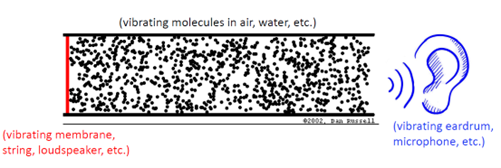
\includegraphics[width=0.8\textwidth]{images/1_8.png}
\end{figure}

In the case of a longitudinal wave in a gas, these are pressure waves. If you could take a snapshot of the distribution of molecules as sound propagates through the air, you would see regions of compression (high pressure and density) and rarefaction (low pressure and density). These areas of compression and rarefaction alternate due to the transfer of momentum between molecules. A sound wave is, in fact, a very small variation in the overall atmospheric pressure. The distance between two consecutive compressions (or two consecutive rarefactions) represents the wavelength.

\begin{figure}[H]
    \centering
    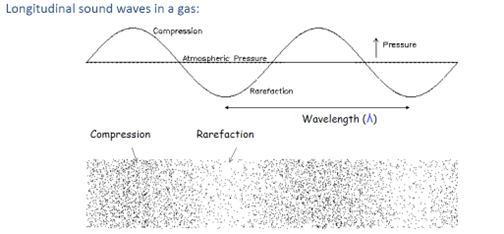
\includegraphics[width=0.8\textwidth]{images/1_9.png}
\end{figure}

The molecules are not transported by the wave; they only oscillate back and forth. By doing this, they create a modulation in the conditions of the medium, allowing the wave to propagate. Therefore, the wave transports energy and momentum, but not the material itself. It is the perturbation, or local change in pressure, that initiates the wave-like motion and propagates through the medium. This motion occurs on top of the chaotic thermal motion of the fluid: the faster the molecules move randomly, the higher the temperature of the gas. The sound wave, however, introduces an additional layer of ordered motion on top of this random molecular movement.

\subsection{Description of Vibrations}

Today, we focus on point masses subject to restoring forces. Consider a point mass \( m \) attached to a spring with a spring constant \( k \). If we release the mass, it begins to oscillate. Observing its position over time, we see that the oscillation decreases due to friction or damping, meaning it is not a perfectly periodic oscillation—this is called a \textbf{free oscillation}. We can calculate the velocity by differentiating the position of the mass over time \(\vec{v} = \frac{\partial \vec{s}}{\partial t} \) where \(\vec{s}\) is the displacement. A free damped oscillation means no external forces act on the system (the system starts from equilibrium).

\begin{figure}[H]
    \centering
    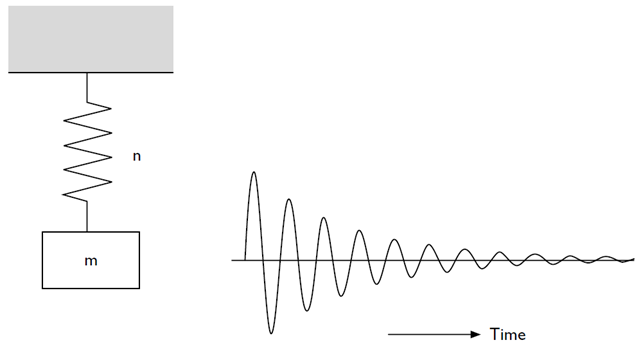
\includegraphics[width=0.6\textwidth]{images/1_11_1.png}
    \caption{generic damped oscillation}
\end{figure}

For a periodic system, the displacement repeats itself after a specific period \( T \). A harmonic oscillation is a type of periodic oscillation that follows a sine or cosine function.
\[s(t) = \hat{s} \cos(\omega t + \phi) \]
The argument \( \omega \) is the angular frequency, while \( \phi \) is the initial phase, a fixed parameter determined by the initial conditions of the system. The second free parameter is the maximum displacement \( \hat{s} \). The period \( T \) is the time it takes to complete one full cycle, while the frequency \( f \) is how many cycles occur per second. If we multiply the frequency by \( 2\pi \), we obtain the angular frequency \( \omega \) in radians per second. It's a good habit to express frequency as \( 1/s \) or Hz, and angular frequency as radians per second (rad/s). Note that radians are a pure number, not a unit of measurement.
\[f = \frac{\omega}{2\pi} = \frac{1}{T}\]

\begin{figure}[H]
    \centering
    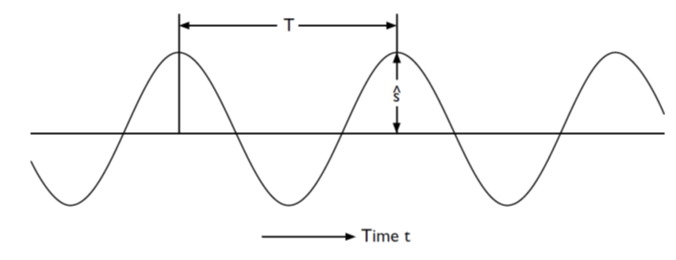
\includegraphics[width=0.6\textwidth]{images/1_11_2.png}
    \caption{periodic (stationary) oscillations}
\end{figure}

We can also encounter random oscillations, such as the motion of molecules in the air when no sound wave is present.

\begin{figure}[H]
    \centering
    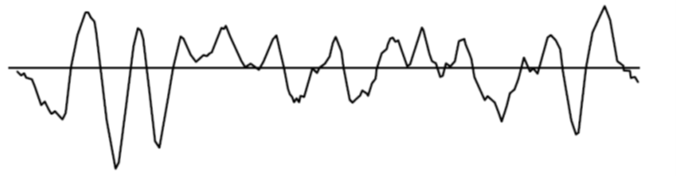
\includegraphics[width=0.6\textwidth]{images/1_11_3.png}
    \caption{random oscillations}
\end{figure}

\subsection{Average and Magnitude of Vibrations}

In general, we use the equilibrium position of the oscillating system as the reference point for displacement. This means that if you average the displacement over a long period of time, it will be zero. For a periodic oscillation, the average displacement over one complete period is also zero.
\[\langle s \rangle = \frac{1}{t_0} \int_0^{t_0} s(t) \, dt \]
\[
t_0 = T \quad \text{for periodic oscillations,} \quad t_0 \to \infty \quad \text{for random oscillations.}
\]
where 
To quantify how large the oscillations (displacements) are, we need to take the average of a positive quantity. This can be done by averaging the square of the displacement (to ensure all values are positive), or by taking the absolute value. This method gives us a meaningful measure of the magnitude of oscillations, often referred to as the root mean square (RMS) value.
\[\langle s^2 \rangle = \frac{1}{t_0} \int_0^{t_0} [s(t)]^2 \, dt = \tilde{s}^2\]

\subsection{Complex Notation of Harmonic Vibrations}

To describe these oscillations, we use complex notation, the typical notation for waves. Harmonic oscillations are the projections of a periodic circular motion: the projection onto the horizontal axis gives us a sine or cosine function. The best way to visualize this is by considering the complex plane, where the horizontal axis represents the real part of a complex number, and the vertical axis represents the imaginary part. If we look at a point in this plane, the distance from the center (origin) to the point (represented as an arrow or vector) is the modulus (or magnitude) of the complex number. The projection of this point onto the horizontal axis is the real part, and the projection onto the vertical axis is the imaginary part. The angle between the arrow and the real axis is called the phase. Euler’s formula connects the complex exponential to these components: \( e^{j\omega t} \), where the real part corresponds to \( \cos(\phi) \), and the imaginary part corresponds to \( \sin(\phi) \). This is how we relate complex notation to harmonic oscillations.

\begin{figure}[H]
    \centering
    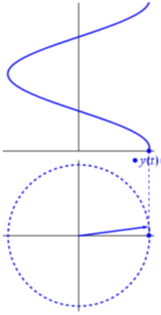
\includegraphics[width=0.2\textwidth]{images/1_13.png}
\end{figure}

The goal is to transition from real-number notation to a form that can be expressed using complex numbers. If we look at the periodic oscillation function \(s(t) = \hat{s} \cos(\omega t + \phi)\), we realize that the cosine is simply the real part of the complex exponential  \(s(t) = \text{Re} \left\{ \hat{s} e^{j(\omega t + \phi)} \right\}\), where the phase (of the complex number) is not just a constant number, but a function of time, meaning that the phase increases linearly over time. As a result, the arrow (or vector) representing the complex number rotates with an angular frequency (also called angular velocity when describing circular motion). This rotating vector in the complex plane is called a phasor. By studying the system in the complex domain, we can perform calculations more easily. Once we have the solution, we return to the real domain. The use of complex numbers simplifies the math, which is why we employ them. In some textbooks, it is assumed without explicitly stating that we are always taking the real part of the complex number \(\tilde{s}(t) = \hat{s} e^{j(\omega t + \phi)}\). The projection of the rotating vector onto the horizontal (real) axis corresponds to the mechanical oscillation we observe.

\begin{figure}[H]
    \centering
    \begin{minipage}{0.4\textwidth}
        \centering
        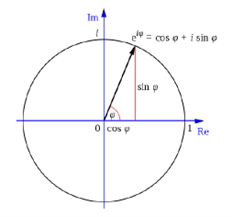
\includegraphics[width=\textwidth]{images/1_14_1.png}
    \end{minipage}%
    \hfill
    \begin{minipage}{0.4\textwidth}
        \centering
        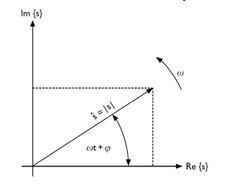
\includegraphics[width=\textwidth]{images/1_14_2.png}
    \end{minipage}
\end{figure}


\vspace{1cm}
Let's look at some examples, particularly regarding differentiation in both real and complex notation. We know that the derivative of the displacement \( s(t) \) gives us the velocity \( v(t) \). The difference between the two notations is how we express this relationship: in real notation, velocity is written as a function of displacement, while in complex notation, velocity is proportional to displacement. Both notations convey the same idea: a sine function is 90 degrees out of phase with a cosine function. When you multiply a complex number by the imaginary unit \( i \), it effectively shifts the phase by 90 degrees.
\[ \text{Real notation:} \quad s(t) = \hat{s} \cos(\omega t + \phi) \quad v(t) = -\omega \hat{s} \sin(\omega t + \phi)
\]
\[ \text{Complex (phasor) notation:} \quad s(t) = \hat{s} e^{j(\omega t + \phi)}
\quad
v(t) = j \omega \hat{s} e^{j(\omega t + \phi)} = j \omega s
\]

In complex notation, differentiation is simplified as multiplication; similarly, instead of integrating, you divide.
\[\frac{d}{dt} \leftrightarrow j \omega
\quad
\int \, dt \leftrightarrow \frac{1}{j \omega}
\]
\vspace{1cm}
Let's consider a second example. Imagine we have two harmonic signals with the same amplitude but slightly different phases. If we sum these two signals, we observe that when the oscillations are perfectly in phase, the overall oscillation becomes larger, and when they are out of phase, the amplitude becomes smaller. This variation in amplitude changes over time. This mechanism is used in digital tuners for instruments. When two notes are very close in frequency but not the same, we hear a phenomenon called beats. Beating is a type of volume modulation that occurs when two frequencies are very close, but not identical. When summing the two signals, we obtain the complex exponential of an oscillation at frequency \( \omega \) (which is the average frequency of the two signals) and the cosine of \( \Delta \omega \) (the difference in frequencies) acts as an amplitude modulator for the complex exponential. This creates the effect of amplitude modulation, which is what we perceive as beats.

\begin{figure}[h]
    \centering
    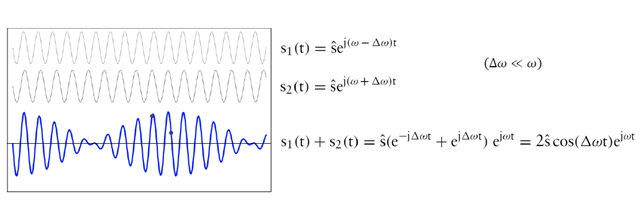
\includegraphics[width=0.9\textwidth]{images/1_16.png}
\end{figure}

\subsection{Oscillation of a Simple Resonator}

Now we approach the equation of motion using complex notation. Consider a simple resonator: a mass, a spring, and no friction acting on the system.

\begin{figure}[h]
    \centering
    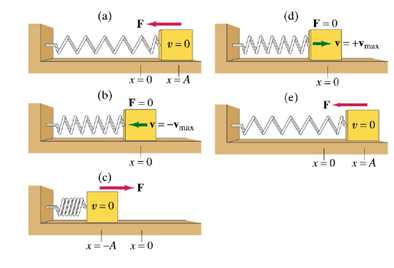
\includegraphics[width=0.7\textwidth]{images/1_17.png}
    \caption{Simple Resonator}
    \label{fig:1_17}
\end{figure}

Any analysis starts with Newton's laws: we need to identify the forces acting on the mass. In this case, the only force is the elastic force from the spring: \[F = -kx = m\frac{d^2x}{dt^2}\]
. Solving the differential equation of motion means finding the function that describes the displacement \( x(t) \) as a function of time.

When we release the mass, it starts with zero velocity and maximum displacement, which corresponds to maximum force (and acceleration). As the mass moves towards the center (the equilibrium position), the spring is at rest, so there is no force acting on the mass, which means zero acceleration and maximum velocity, with zero displacement. Every time the mass is at the extremes the acceleration is at its maximum, the displacement is also at its maximum, but the velocity is zero; while in the center, the velocity is maximum, and the displacement is zero.  This motion can be described with a second-order differential equation, meaning that to find the displacement, we need to integrate twice. Each time we differentiate, we add a constant to the solution, so the general solution will have two free parameters. We need two initial conditions to determine the values of these parameters for the specific case. For example, if we pull the spring by a distance \( A \) and then let it go, the initial conditions are \( x(0) = A \) and \( v(0) = 0 \). 

To solve this, we use a general method involving exponential notation, which is very powerful in physics. If we have some intuition about the expected solution, we can make an educated guess and then substitute it into the equation. If the guess is correct, it will satisfy the differential equation. Let’s assume this is a free oscillation, which means harmonic motion. We can write the displacement \( x(t) \) in a general form as an amplitude \( \hat{x} \) multiplied by an exponential function: \[x(t) = \hat{x} e^{gt}\]. Substituting this expression into the equation of motion simplifies it to a form where we can solve for the parameters: \[
-k \hat{x} e^{gt} = m \hat{x} g^2 e^{gt}
\]
From the solution, we obtain \( g \), the natural frequency of oscillation for the spring-mass system.
\[
g^2 + \frac{k}{m} = 0 \quad \to \quad g = \pm j \sqrt{\frac{k}{m}}
\]
Plugging \( g \) back into the guessed solution gives us the final solution. \[
\tilde{x}(t) = \hat{x} e^{\pm j \sqrt{\frac{k}{m}}t} \quad
x(t) = \text{Re}[\tilde{x}(t)] = \hat{x} \cos\left(\sqrt{\frac{k}{m}}t + \phi\right)
\]There are two possible solutions: one with a positive and one with a negative exponent in \( x(t) \). These two solutions correspond to the two directions in which the oscillation can occur (one going forward in time, the other backward). The general solution is a linear combination of both solutions, which means that we combine them with two free parameters to form the overall solution. In real life, we deal with real numbers, not complex numbers: since we're using complex exponential functions to solve the equation, we need to extract the real part of the solution to describe the actual physical motion. Both the solutions have real parts that are related to cosine and sine functions; so, when we take the real part of the general solution, we end up with a linear combination of sine and cosine functions. A key property in trigonometry is that any linear combination of cosine and sine can be written as a single cosine (or sine) function with a phase shift. This is more convenient because it simplifies the expression to just one trigonometric function, where the phase shift \( \phi \) is determined by the initial conditions (like where the mass starts and how fast it's moving).

\subsection{Oscillation of a Simple Damped Resonator}

Now we consider a simple damped resonator, a mass-spring system with damping, meaning there is viscous friction acting on the system.

\begin{figure}[h]
    \centering
    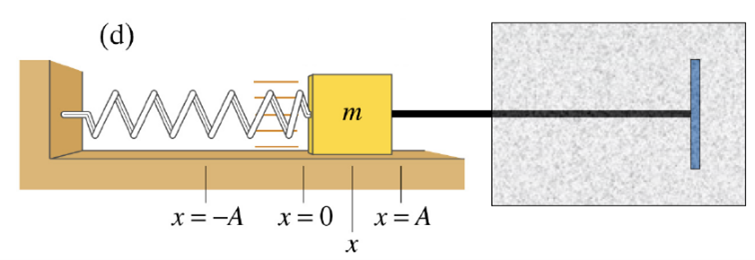
\includegraphics[width=0.6\textwidth]{images/1_19.png}
    \caption{Damped Resonator}
    \label{fig:1_19}
\end{figure}

In this case, the forces acting on the mass include the elastic force from the spring and the viscous damping force (proportional to velocity, with a viscous damping coefficient).
\[
-kx - \beta \frac{dx}{dt} = m\frac{d^2x}{dt^2}
\]
Our guess for the solution is a function \( x(t) \) that appears in the equation directly (elastic force), as a first derivative (friction), and as a second derivative (mass). The differential equation requires that a linear combination of these terms equals zero. This condition can only be satisfied with an exponential function as a solution. 
\[
x(t) = x_0 e^{gt}
\]
Now we plug it into the differential equation. After simplification, we arrive at an equation that must be satisfied for our guessed solution to work. This is a second-order differential equation that imposes a condition on \( g \) (the exponent in the solution), which depends on the physical parameters of the system.
\[
-kx_0 e^{gt} - \beta x_0 g e^{gt} = mx_0 g^2 e^{gt}
\]

The solutions for \( g \) have both real and imaginary components. Oscillations only occur if the damping coefficient \( \beta \) is low enough for the term under the square root to be negative (which gives the imaginary part). 
\[
g^2 + \frac{\beta}{m} g + \frac{k}{m} = 0 \quad \to \quad g = -\frac{\beta}{2m} \pm \sqrt{\frac{\beta^2}{4m^2} - \frac{k}{m}} = -\frac{\beta}{2m} \pm j \sqrt{\frac{k}{m} - \frac{\beta^2}{4m^2}}
\]
When we substitute the values of \( g \) back into the solution, the resulting form resembles the solution for the undamped oscillator, but with a dumping term \(-\frac{\beta}{2m}t\) and a shift term \( \frac{\beta^2}{4m^2}t \)
\[
x(t) = x_0 e^{-\frac{\beta}{2m}t} e^{\pm j \sqrt{\frac{k}{m} - \frac{\beta^2}{4m^2}}t}
\]
The additional damping term disappears as the damping coefficient \( \beta \) approaches zero, returning to the earlier case of a simple resonator. Essentially, damping introduces a small correction to the natural frequency of oscillation, slightly shifting the system’s resonance.

The key novelty here is the first exponential term in the solution, which represents a real exponential decay envelope. 

\begin{figure}[h]
    \centering
    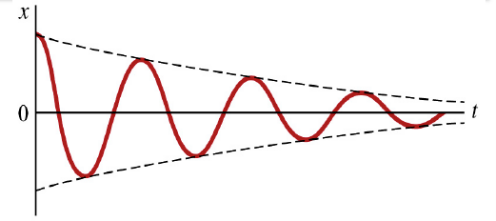
\includegraphics[width=0.4\textwidth]{images/1_20_2.png}
\end{figure}

This term modulates the amplitude of the oscillation over time (as we said, if \( \beta \) approaches zero, the exponential decay disappears, and we return to the undamped case). Damping is not always viscous. It can arise from contact damping due to direct interaction between surfaces. The primary effect of damping, regardless of its origin, is the reduction of oscillation amplitude over time. However, the physical origin of the damping changes the shape of the envelope modulating the oscillations.

\subsection{Oscillation of a Forced Damped Resonator}

Now we add an external force to the system with damping and a spring, resulting in a forced damped resonator. 
\begin{figure}[h]
    \centering
    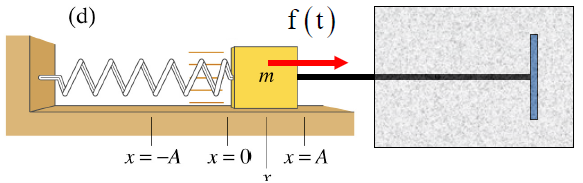
\includegraphics[width=0.6\textwidth]{images/1_21_1.png}
\end{figure}
Three forces act on the mass: the elastic force from the spring, the viscous damping force, and the external force.
\[
-kx - \beta \frac{dx}{dt} + f(t) = m \frac{d^2x}{dt^2}
\]
The solution depends on the analytical expression of the external force \( f(t) \) over time, so we need to specify how the force varies with time to solve the equation. In this case, the external force is a harmonic periodic force. 
\[
f(t) = \hat{f} e^{j\Omega t}
\]
The system has a natural oscillation frequency \( \Omega_0 \), but when we add the external force, it introduces another frequency. Therefore, we have two frequencies: one from the resonator \( \Omega_0 \) (natural frequency) and one from the external force (driving frequency) \( \Omega \). If the system is already oscillating and we turn on the harmonic force, at first, we observe chaotic motion. Over time, the natural oscillations fade out due to damping, as all the initial energy of the system is dissipated. The only energy remaining in the system comes from the external force. If we wait long enough, the natural oscillations completely disappear, and the system settles into a steady-state regime where it oscillates solely at the frequency of the external force. In this regime, the motion becomes periodic because the driving force is the only input.

To study the steady-state oscillation, we can guess a solution \( x(t) \) that takes the form of a harmonic oscillation at the frequency of the external force.
\[
x(t) = \hat{x} e^{j(\Omega t + \Phi)}
\]
This oscillation is generally not in phase with the force (the initial phase \( \Phi \) depends on the system, but we can assume the external force starts with zero phase). The resulting equation is complex: one part involves the real components, and another involves the imaginary components. Solving these equations gives us the amplitude and phase of the oscillation as functions of the system’s parameters.
\[
|\hat{x}(\Omega)| = \frac{\hat{f}}{\sqrt{m^2(\Omega_0^2 - \Omega^2)^2 + \beta^2\Omega^2}}
\quad
\tan{\phi} = -\frac{\beta\Omega}{k - m\Omega^2}
\]

The amplitude of the oscillation increases with the amplitude of the external force. In the denominator of the solution, the relationship between the frequency of the force \( \Omega \) and the natural frequency of the free oscillation \( \Omega_0 \) plays a crucial role. When these two frequencies match, the amplitude becomes very large (\( \Omega_0^2 - \Omega^2 \to 0, |x(\Omega)| \to \infty \)). If there is no damping, the amplitude theoretically goes to infinity (\( \beta = 0, |x(\Omega)| = \infty \)); this is resonance. Resonance occurs when the external force drives the system at its natural frequency, resulting in a large response. However, if the external force’s frequency is far from the natural frequency, the oscillations are small (\( \Omega_0^2 - \Omega^2 \to \infty, |x(\Omega)| \to 0 \)). If damping is too high, resonance does not occur (\( \beta \to \infty, |x(\Omega)| \to 0 \)).

\begin{figure}[h]
    \centering
    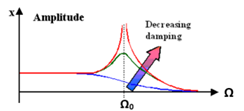
\includegraphics[width=0.5\textwidth]{images/1_21_2.png}
\end{figure}

The phase of the oscillation also depends on the frequency. At low frequencies (below the natural frequency), the phase is zero, meaning the oscillation is in phase with the force. At very high frequencies (much larger than the natural frequency), the phase approaches \( -\pi \), meaning the oscillation is completely out of phase with the force. At resonance, the phase is \( -\pi/2 \), indicating the displacement lags the force by a quarter of a cycle.

\begin{figure}[h]
    \centering
    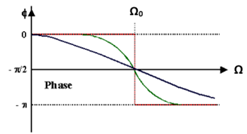
\includegraphics[width=0.5\textwidth]{images/1_21_3.png}
\end{figure}

If we push the system back and forth at low frequencies, the oscillation follows our movement (imagine gently pushing a swing. The swing movement follows your rhythm). At very high frequencies, the oscillation occurs counterphase to the external stimulus, meaning it moves opposite to the applied force (imagine shaking the swing quickly, and it moves in the opposite direction to your push). The oscillation is generally not in phase with the external force unless specific conditions are met.




\subsection{mechanical impedance}

The impedance of a system defines how the system responds to a stimulus. In the case of a mechanical system, we apply a force and evaluate how large the mechanical response is, typically by measuring the velocity of the system. 

To evaluate the mechanical impedance \( Z(\omega) \) of a forced damped oscillator, we rewrite the equation of motion in terms of velocity \( v(t) \).
\[
-kx - \beta \frac{dx}{dt} + f(t) = m \frac{d^2x}{dt^2} \quad \to \quad -k\frac{v}{j\omega} - \beta v + f = j\omega mv
\]
Using these relationships, we derive the expression for impedance:
\[
Z(\omega) = \frac{f}{v} = j\omega m + \beta + \frac{k}{j\omega}.
\]
Where \( \omega \) is the angular frequency of the external force, \( m \) is the mass, \( \beta \) is the damping coefficient, \( k \) is the spring constant. 



Impedance \( Z(\omega) \) depends on the frequency of the external force \( \omega \) and is a complex number because the mechanical response of the system, represented by the velocity \( v(t) \), is generally not in phase with the applied force \( f(t) \). This phase shift occurs due to the interplay between inertia (\( m \)), damping (\( \beta \)), and the elastic restoring force (\( k \)). The phase shift reflects how the system responds to the applied force: at low frequencies, the response closely follows the force, while at high frequencies, the response lags due to inertia.


We can visualize \( Z(\omega) \) in the complex plane.












The impedance \( Z(\omega) \) can be expressed as:
\[
Z(\omega) = \beta + j \, \frac{m}{\omega} (\omega^2 - \omega_0^2),
\]
where \( \omega \) is the angular frequency of the external force, which characterizes the rate at which the force oscillates over time, while \( \omega_0 = \sqrt{\frac{k}{m}} \) is the natural angular frequency of the system, it represents the frequency at which the system oscillates in the absence of damping and external forces.


The real part of \( Z(\omega) \), given by \( \text{Re}(Z) = \beta \), remains constant because it depends solely on the damping coefficient. The imaginary part, \( \text{Im}(Z) = \frac{m}{\omega} (\omega^2 - \omega_0^2) \), varies with \( \omega \), causing \( Z(\omega) \) to describe a curve in the complex plane.
\begin{itemize}
    \item For \( \omega < \omega_0 \), the imaginary part is negative because \( \omega^2 - \omega_0^2 < 0 \). This indicates that the elastic restoring force dominates over inertia in this frequency regime.
\item At \( \omega = \omega_0 \), the imaginary part becomes zero since \( \omega^2 - \omega_0^2 = 0 \). At this frequency, the system is at resonance, and the impedance is purely real, equal to \( \beta \).
\item For \( \omega > \omega_0 \), the imaginary part is positive because \( \omega^2 - \omega_0^2 > 0   \). In this case, the inertial effects dominate over the elastic restoring force.
\end{itemize}




\begin{figure}[H]
    \centering
    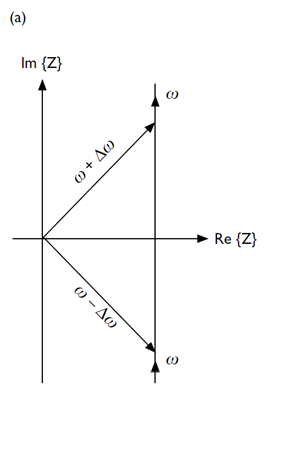
\includegraphics[width=0.3\textwidth]{images/1_22_1.png}
\end{figure}




\[
Y(\omega) = \frac{1}{Z(\omega)}
\]
The admittance \( Y(\omega) \) is the reciprocal of the impedance and is used to analyze resonance behavior. At resonance, the system exhibits a large mechanical response even to small forces. The admittance reaches a peak at the resonance frequency. 
If damping \( \beta \) is small, the peak of admittance is sharp, indicating strong resonance.
The width of the resonance peak, denoted as \( \Delta \omega = (\omega_2 - \omega_1) \), is defined as the range of frequencies where the amplitude of the response is at least \( y_{\text{max}} / \sqrt{2} \), where the maximum response \( y_{\text{max}} \) occurs at the resonance frequency \( \omega_0 \).
It can be demonstrated that the frequencies \( \omega_1 \) and \( \omega_2 \) are those where the real and imaginary parts of the impedance \( Z(\omega) \) are equal in magnitude. At these frequencies, the dissipative term (\( \beta \)) and the inertial-elastic term (\( j(\omega m - \frac{k}{\omega}) \)) balance each other, contributing equally to the system's response.
\begin{figure}[H]
    \centering
    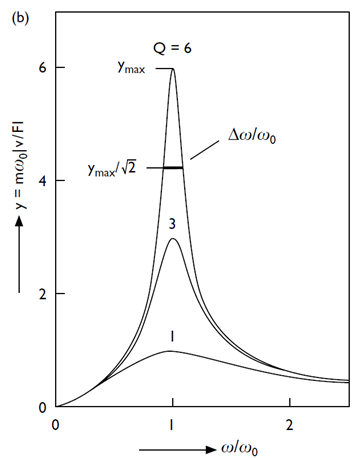
\includegraphics[width=0.4\textwidth]{images/1_22_2.png}
\end{figure}


The quality factor \( Q \) quantifies the strength of resonance and is defined as:
\[
Q = \frac{\omega_0}{\Delta \omega} = \frac{\omega_0}{\beta / m} = \frac{m \omega_0}{\beta}.
\]
where \( \omega_0 \) is the resonance frequency. The quality factor is inversely proportional to the damping coefficient \( \beta \). Larger damping results in a broader peak and a smaller quality factor.

\subsection{Electromechanical analogies}
There are many connections between concepts in the mechanical domain and those in electrical engineering. This relationship arises because every mechanical oscillating system is described by a second-order differential equation, just as many electrical circuits are. Whenever different systems are governed by mathematically similar equations, parallels can be drawn between the parameters of both systems.

Let’s explore the relationships between circuit elements and their mechanical analogs. Starting with the following equations:
\begin{align}
    U_R &= R \cdot I, \label{eq:resistor} \\
    U_C &= \frac{1}{C} \int I \, dt, \label{eq:capacitor} \\
    U_L &= L \frac{dI}{dt}, \label{eq:inductor}
\end{align}
we can create the following analogies:

\begin{figure}[H]
    \centering
    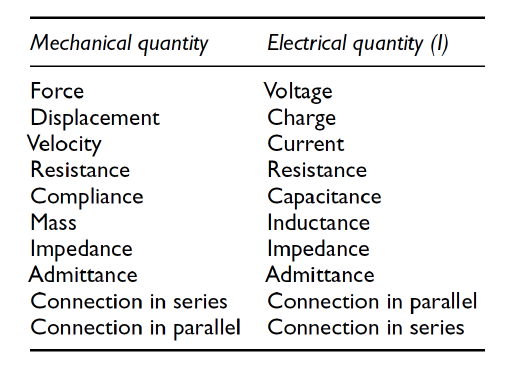
\includegraphics[width=0.4\textwidth]{images/1_23.png}
\end{figure}

The first equation \eqref{eq:resistor} describes dissipation: just as the voltage across a resistor is proportional to the current, the force in a mechanical system is proportional to the velocity. Here, resistance \( R \) is analogous to the coefficient of viscous damping \( \beta \). The second equation \eqref{eq:capacitor} describes elastic behavior: the voltage across a capacitor, which is proportional to the charge, corresponds to the displacement in a mechanical system. The third equation \eqref{eq:inductor} describes inertia: the voltage across an inductor is proportional to the rate of change of current, just as the force due to mass is proportional to the acceleration.

Connections in series in an electrical system correspond to elements sharing the same current. Similarly, in a mechanical system, elements connected in series share the same velocity, meaning all the mechanical elements move together. In contrast, mechanical elements connected in parallel experience the same displacement, analogous to the same voltage across parallel electrical elements.
\begin{figure}[H]
    \centering
    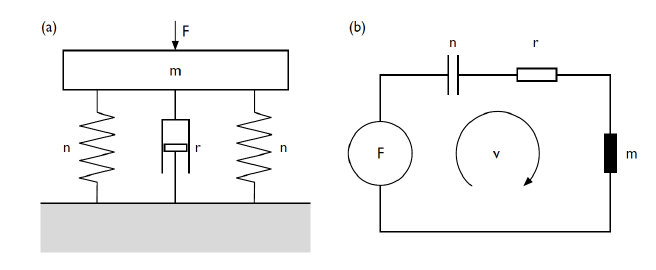
\includegraphics[width=0.6\textwidth]{images/1_24_1.png}
     \caption{Series configuration}
    \label{fig:mechanical_parallel_series_1}
\end{figure}
\begin{figure}[H]
    \centering
    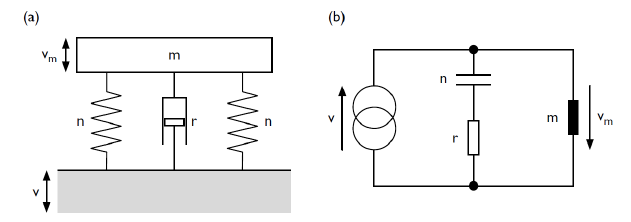
\includegraphics[width=0.6\textwidth]{images/1_24_2.png}
     \caption{Parallel configuration}
    \label{fig:mechanical_parallel_series_2}
\end{figure}
The system \ref{fig:mechanical_parallel_series_1} consists of a mass attached to a spring and a damper, with a force applied to the mass. The system \ref{fig:mechanical_parallel_series_2} is similar but involves a fixed velocity. In practical systems, an external force can be applied either with a known force or with a known velocity. In electromechanical analogies, this corresponds to using either a voltage generator or a current generator.

In the first example \ref{fig:mechanical_parallel_series_1}, the three elements (spring, damper, and mass) are connected in series. The capacitance represents the spring, the resistance represents the damper, and the inductance represents the mass. When elements are connected in series, they are crossed by the same current, which in the mechanical analogy means that all elements share the same velocity. If the mass is displaced by an applied force, all the components, the spring, damper, and mass, move by the same quantity, having the same velocity but experiencing different forces depending on their physical properties. Considering two elements with different masses connected in series, if a force is applied to the first element, the following element in series will experience a different force because the applied force is distributed based on their respective masses. However, both elements will share the same acceleration as they are mechanically connected.

In the second example\ref{fig:mechanical_parallel_series_2}, the inductor (representing the mass) is connected in parallel with the other two elements, the spring and the damper. In this configuration, all elements experience the same velocity since they are parallel. There is no external force, so the force applied to the first element, the mass, is distributed equally to the spring and the damper.

\subsection{Power in Oscillatory Systems}

When a force is applied to make a system oscillate, work is being done, and energy is expended. The power required to maintain the oscillations is an important quantity to consider. Power is the rate at which work is done, and work is defined as \( L = f \cdot s \). Since displacement over time is velocity, \( v = \frac{ds}{dt} \), power can be expressed as \( P = f \cdot v \), where \( P \).
\[
P = \frac{\delta L}{dt} = f \cdot \frac{ds}{dt} = f \cdot v
\]


In this system, the force and displacement are oscillatory and generally have different phases.
\[
f(t) = \text{Re}\left[\hat{f} e^{j\Omega t}\right] = \hat{f} \cos(\Omega t),
\]
\[
x(t) = \text{Re}\left[\hat{x} e^{j(\Omega t + \Phi)}\right] = \hat{x} \cos(\Omega t + \Phi),
\]
The velocity, being the time derivative of displacement, also oscillates at the same frequency as the force but with its own phase shift.
\[
v(t) = -\Omega \hat{x} \sin(\Omega t + \Phi) = \hat{v} \cos(\Omega t + \Phi').
\]The power expression can thus be expanded:
\[
P = f \cdot v = \frac{1}{2} \hat{f} \hat{v} \left[\cos(\Phi') + \cos(2\Omega t + \Phi')\right]
\]

The larger the force, the greater the velocity, and consequently, the greater the power. Increasing the displacement results in more work being done.
This expression contains two terms: The first term, \( \cos(\Phi') \), is constant and is called the \textbf{active power}. It represents the average power required to maintain the oscillation.,The second term, \( \cos(2\Omega t + \Phi') \), oscillates over time at twice the frequency of the force. This is the \textbf{reactive power}, which periodically goes from positive to negative. Its average over time is zero, meaning this energy flows back and forth between the system and the external source without contributing to sustained oscillation. 
The active power is the energy spent to keep the oscillations alive, while the reactive power represents energy temporarily stored and returned to the system.


\subsection{Fourier Analysis}

Fourier analysis allows any periodic signal to be decomposed into harmonic functions. If we consider a general periodic signal \( s(t) \), it can always be expressed as a series of discrete terms, where each term is a complex exponential. 
\[
s(t + T) = s(t) = \sum_{n=-\infty}^\infty C_n e^{j\frac{2\pi n t}{T}} \quad \text{where} \quad C_n = \frac{1}{T} \int_0^T s(t) e^{-j\frac{2\pi n t}{T}} \, dt
\]
Each term represents an oscillation with a frequency \( \frac{2\pi}{T} \), the fundamental frequency, and its harmonics. In this representation, \( n \) is a natural number, so we have oscillatory terms at \( \omega = \frac{2\pi}{T} \), \( \frac{4\pi}{T} \), \( \frac{6\pi}{T} \), and so on. The Fourier series converges to the original periodic signal as the number of terms approaches infinity. Depending on the nature of the signal, a specific number of harmonics may be sufficient to describe it accurately. Mathematically, the set of harmonic functions forms a basis for representing any periodic signal through linear combinations. Thus, any periodic function, even if not inherently harmonic, can be expressed as a sum of harmonic functions.
Understanding how a system responds to periodic forces allows us to predict its behavior for any arbitrary periodic signal. The Fourier coefficients \( C_n \) are generally complex, and if the signal \( s(t) \) is real, then the negative coefficients are the complex conjugates of the positive coefficients:
\[
C_{-n} = C_n^*.
\]


For non-periodic signals, we can generalize the concept of Fourier analysis by introducing \( \Delta \omega \), the spacing between two harmonics, which is equal to \( \omega_0 = \frac{2\pi}{T} \), the fundamental frequency. Starting from the Fourier series for a periodic signal, we multiply by \( \Delta \omega \) and transition from a discrete summation to an integral, moving from discrete variables to continuous ones. This transition effectively replaces the discrete set of harmonic frequencies \( n\omega_0 \) spaced \( \Delta \omega \), which describe finite periodicity, with a continuous set of frequency values \( \omega \) spaced by \( d\omega \) (infinitesimal distance). In doing so, we move from describing periodic signals to describing any arbitrary non-periodic signals.

\[
s(t) = \sum_{n=-\infty}^\infty \frac{C_n}{\omega_0} e^{j\omega t} \Delta \omega \to \int_{-\infty}^\infty C(\omega) e^{j\omega t} d\omega \quad \text{for } T \to \infty \]
\[ \text{where}  \quad
C(\omega) = \frac{1}{2\pi} \int_{-\infty}^\infty s(t) e^{-j\omega t} dt
\]
Harmonic functions thus allow us to represent both periodic and non-periodic signals in terms of their frequency components.

\vspace{1cm}

The spectrum represents the frequency content of a sound. For example, if we play the note \( \text{C4} \) fortissimo on a piano, we produce a large number of harmonics, forming a continuous spectrum. The spectrum indicates the contribution of harmonic functions at different frequencies and collectively defines the timbre of the sound. The timbre is influenced by the harmonic content, which depends on how we produce the sound. For instance, playing \( \text{C4} \) pianissimo changes the spectral content, resulting in a different timbre. This shows that the way we touch the string or key significantly alters the harmonic structure and the spectral content of the produced sound.
\begin{figure}[H]
    \centering
    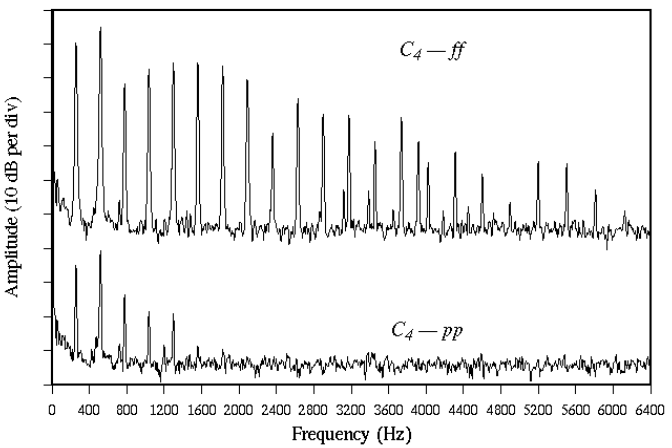
\includegraphics[width=0.6\textwidth]{images/1_29_1.png}
\end{figure}
\vspace{1cm}


Historically, the spectrum of sounds was measured using Helmholtz resonators. These resonators consist of spheres of various sizes, each tuned to a specific acoustic frequency. When a sound wave containing a matching frequency reaches the resonator, it vibrates in resonance. This resonance can be visually observed using systems such as candle flames placed near the resonators; the movement of air caused by the oscillations makes the flame flicker.

In modern times, the spectrum of sound is measured using electronic and digital methods. The sound is first transduced into an electrical signal, which can be filtered and analyzed to calculate the spectrum.

Today, we commonly sample the sound digitally and apply a Fast Fourier Transform (FFT) algorithm. The FFT computes the integral of the signal \( s(t) \) in real time, providing the spectral coefficients \( C(\omega) \) that represent the frequency content of the sound.

\section{The wave equation}
\label{sec:wave_equation} 

In \ref{sec:introduction_to_vibrations}  we localized oscillations caused by a restoring force. In \ref{sec:wave_equation} we focus on the differential equations describing wave propagation. We will examine how any perturbation along a string propagates as a wave, extending the discussion from 1D strings to 2D membranes.
\begin{equation} \label{eq:wave_equation}
    f = f(x \pm vt) \quad \forall f
\end{equation}
This expression describes a wave that propagates in space and oscillates in time, specifically in one dimension. $f$ can be any function, meaning that we can have full freedom in choosing the shape of the wave. While we can have any function $f$, the arguments $x$ and $t$ cannot be freely chosen. The function must depend on $x - vt$, where $v$ is the velocity of propagation. Any function whose argument is $x - vt$ will describe a wave. 

Now we consider a perturbation (such as an electric field in free space, waves on the surface of the sea, or the pressure of a fluid giving rise to sound propagation) and a medium (e.g., a string). The perturbation represents the vertical displacement, while the horizontal axis corresponds to propagation. 
\begin{figure}[H]
    \centering
    \begin{subfigure}[b]{0.4\textwidth}
        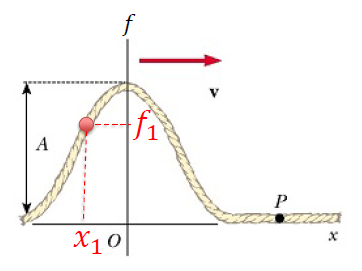
\includegraphics[width=\textwidth]{images/2_2_1.png}
        \caption{t = t1}
        \label{fig:t1}
    \end{subfigure}
    \hfill
    \begin{subfigure}[b]{0.4\textwidth}
        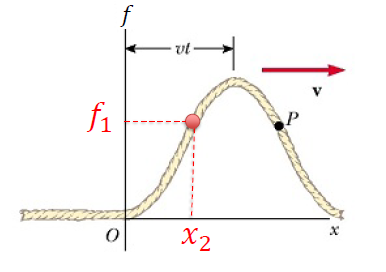
\includegraphics[width=\textwidth]{images/2_2_2.png}
        \caption{t = t2}
        \label{fig:t2}
    \end{subfigure}
\end{figure}
At a certain time $t_1$, we observe the shape of the wave. For instance, if we measure the perturbation at coordinate $x_1$, we find a value $f_1$ corresponding to $x_1$ at $t_1$. 
\[
f_1 = f(x_1 - vt_1)
\]
At a later time $t_2$, the perturbation has moved, and we identify the point $x_2$ where the perturbation still has the same value $f_1$. The relationship between $x_1$ and $x_2$ is such that $x_2 = x_1 + v(t_2 - t_1)$, demonstrating that the perturbation travels at a constant velocity $v$. The value of the perturbation at $x_2$ is the same as it was previously at $x_1$, 
\[
f_2 = f(x_2 - vt_2) = f(x_1 + v(t_2 - t_1) - vt_2) = f_1
\]
meaning the function describes wave propagation: the same perturbation is translated over space without changing its shape. Depending on the direction of propagation, the wave function may depend on $x - vt$ or $x + vt$.\\

The wave equation \(f = f(x \pm vt)\) satisfy the following differential equation:
\[
\frac{d^2 f}{dx^2} = f''(x - vt)
\quad
\frac{d^2 f}{dt^2} = v^2 f''(x - vt)
\quad \to \quad
\frac{d^2 f}{dt^2} = v^2 \frac{d^2 f}{dx^2}
\]
When the second time derivative is proportional to the second spatial derivative, the differential equation describes wave propagation. Any wave function must exhibit proportionality between the second time derivative and the second spatial derivative. The proportionality factor is the square of the velocity of propagation, $v^2$. This is a second-order differential equation, so we expect two solutions. Indeed, the solutions are $x - vt$ and $x + vt$, corresponding to waves propagating in opposite directions. \\

Waves can be viewed from two perspectives: spatial and temporal. If we take a snapshot at a fixed time, we obtain the spatial distribution of the wave at that moment. Alternatively, we can focus on how the wave evolves over time at a fixed point in space. These two perspectives qualitatively appear the same but describe different aspects of the wave. \\

\begin{figure}[H]
    \centering
    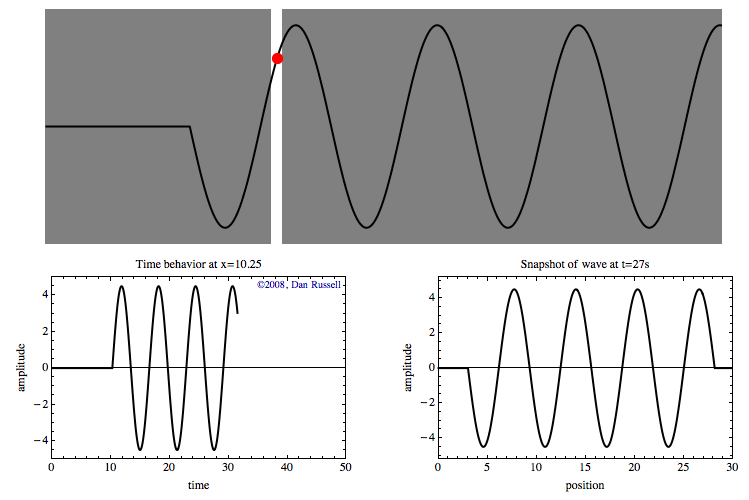
\includegraphics[width=0.8\textwidth]{images/2_4.png}
\end{figure}

\subsection{Transverse and Longitudinal Waves}
Transverse waves are characterized by the propagation of the wave in one direction while the perturbation occurs in a perpendicular direction. For example, tension in a string can produce transverse waves, where the oscillation occurs vertically while the wave propagates horizontally. \\

\begin{figure}[H]
    \centering
    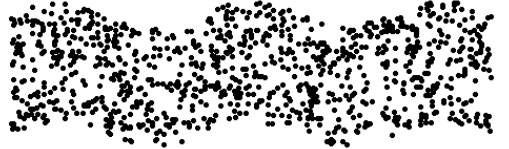
\includegraphics[width=0.5\textwidth]{images/2_5_2.png}
\end{figure}

Longitudinal waves, on the other hand, are characterized by the oscillations of particles occurring in the same direction as the wave propagation. In this case, molecules in the medium collide with one another, transferring energy along the propagation axis. \\

\begin{figure}[H]
    \centering
    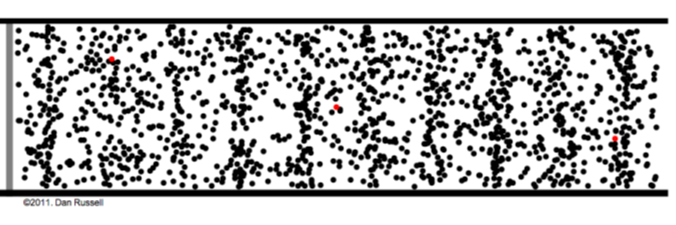
\includegraphics[width=0.5\textwidth]{images/2_5_1.png}
\end{figure}

In summary, transverse waves involve perpendicular perturbations relative to the direction of propagation, whereas longitudinal waves involve parallel oscillations along the propagation direction.\\

Not all waves can be classified strictly as longitudinal or transverse. These are the simplest examples, but in certain fluids with viscosity or in solids, waves can exhibit a mix of longitudinal and transverse components. An example of this is observed on the surface of the sea. The displacement of a single molecule traces a circular motion, which becomes smaller as we move deeper into the sea. 

\begin{figure}[H]
    \centering
    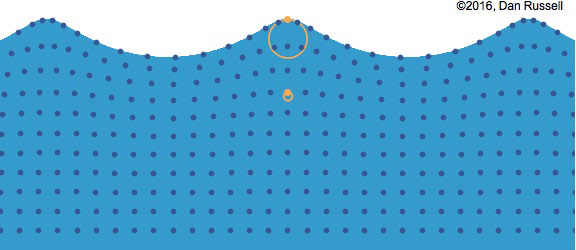
\includegraphics[width=0.5\textwidth]{images/2_6_1.png}
\end{figure}

If the viscosity increases, the motion transitions from circular to elliptical.

\begin{figure}[H]
    \centering
    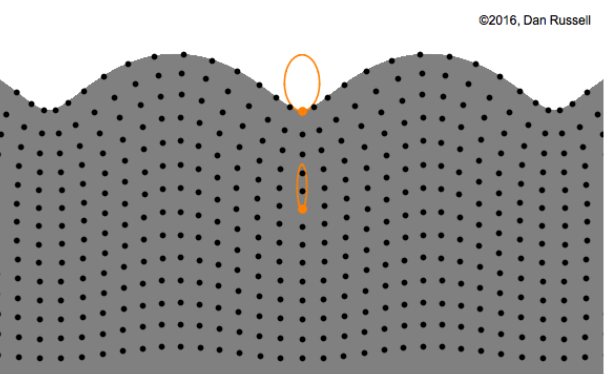
\includegraphics[width=0.5\textwidth]{images/2_6_2.png}
\end{figure}

The mechanism for the propagation of the perturbation in a string is the tension. When the string is perturbed (tilted due to displacement), the tension in the string also tilts, developing a vertical component. This vertical component is balanced by the opposing vertical component from the adjacent segment of the string. This causes one piece of the string to pull down its neighboring segment. 
\begin{figure}[H]
    \centering
    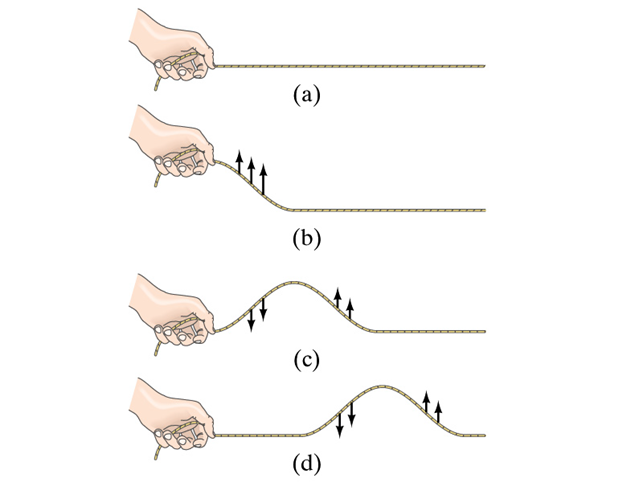
\includegraphics[width=0.5\textwidth]{images/2_7_2.png}
\end{figure}
For all waves, two types of velocities are present: the velocity of wave propagation and the velocity of the perturbed mass element moving as a result of being reached by the wave. For transverse waves, such as those on a string, the perturbed mass element exhibits vertical motion, so we can associate a velocity to the vertical displacement of the perturbed mass, while the wave itself propagates horizontally. Thus, the two velocities are perpendicular. 
\begin{figure}[H]
    \centering
    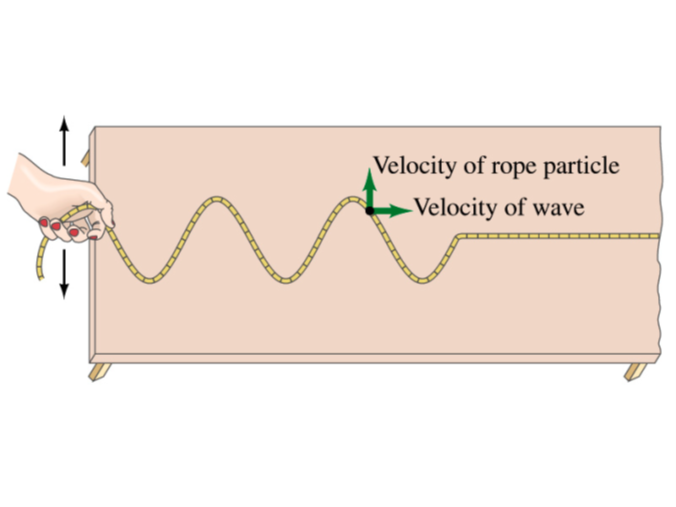
\includegraphics[width=0.5\textwidth]{images/2_7_1.png}
\end{figure}
Notice that the vertical velocity is the time derivative of displacement, while the horizontal wave propagation velocity is constant and not derived from the displacement.

For sound waves, however, both the velocity of molecular oscillation and the wave propagation velocity are in the same direction. 
\\

An analogy to describe the behavior of a string considers the string as a continuum of distributed masses. Each infinitesimal segment of the string is treated as having infinitesimal mass. To simplify, we consider one mass attached to two springs. In this case, the mass can move in two ways: longitudinally and transversely. If we extend this model to two masses, we observe two modes for each type of motion:\\
For longitudinal modes:
     \begin{enumerate}
        \item Both masses oscillate horizontally in phase (both move left or right together).
        \item Both masses oscillate horizontally in counterphase (they move closer and farther apart).
    \end{enumerate}
For transverse modes:
    \begin{enumerate}
        \item Both masses oscillate vertically in phase (both move up and down together).
        \item Both masses oscillate vertically in counterphase (one moves up while the other moves down).
    \end{enumerate}


\begin{figure}[H]
    \centering
    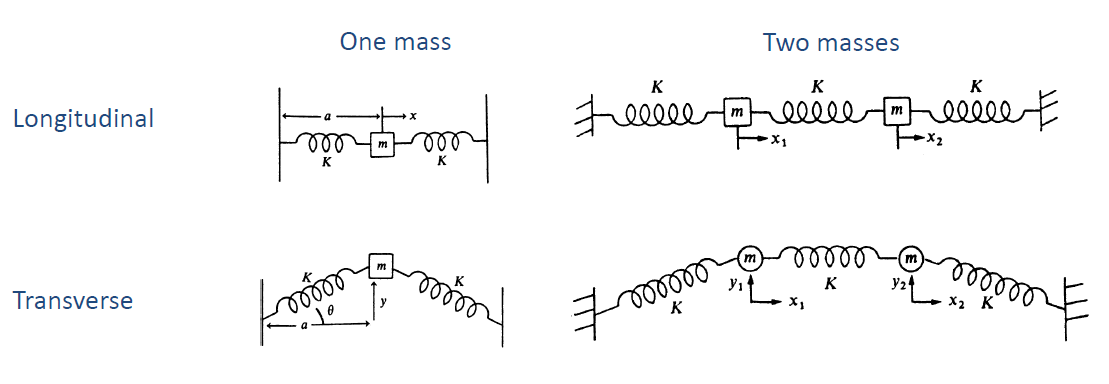
\includegraphics[width=0.8\textwidth]{images/2_8.png}
\end{figure}

If the model is extended to infinite masses (a string), the number of modes increases. For three masses, we observe three longitudinal modes and three transverse modes.\\ 
For transverse modes:
\begin{enumerate}
\item All masses move up and down together.
\item The middle mass remains stationary while the first and third masses oscillate alternately, creating a node in the middle.
\item The three masses alternate between "up-down-up" or "down-up-down" configurations.
\end{enumerate}

The same applies to longitudinal modes, with corresponding nodes appearing as the order increases. The appearance of higher-order modes is associated with the presence of more nodes along the chain.

\begin{figure}[H]
    \centering
    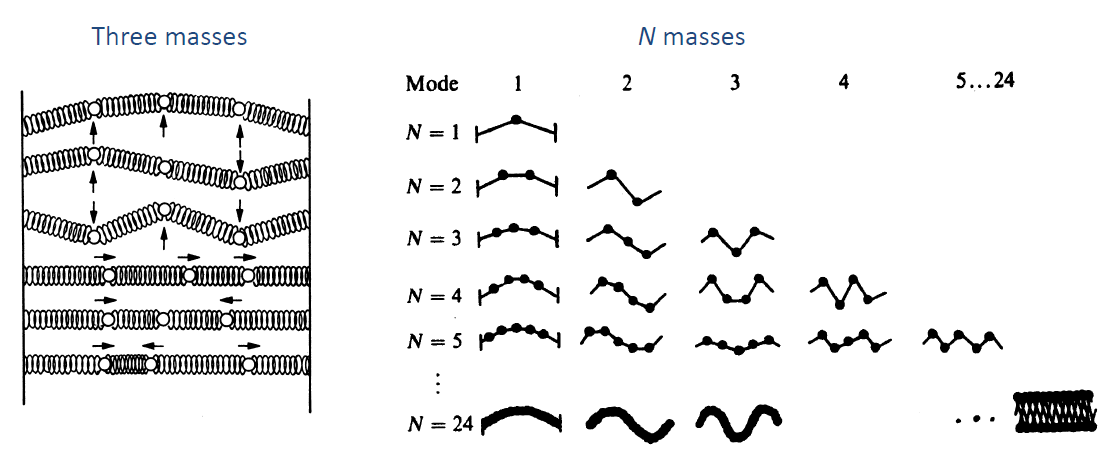
\includegraphics[width=0.8\textwidth]{images/2_9.png}
\end{figure}

\subsection{One dimension waves in infinite strings}

The function \( f \) describing the wave can take any form, meaning the actual analytical shape of \( f \) depends on the initial conditions, including the shape and velocity of the perturbation. 
\begin{figure}[H]
    \centering
    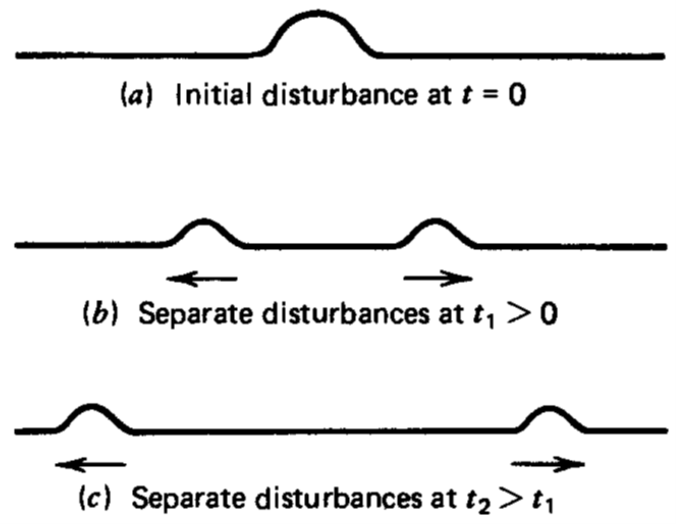
\includegraphics[width=0.4\textwidth]{images/2_10_1.png}
\end{figure}
At \( t = 0 \), an initial disturbance occurs, after which the wave propagates. The solution splits into two parts: one propagating to the left and the other to the right. The differential equation governing this behavior describes the motion of the system. 

Let's consider a string characterized by its linear mass density \(\mu\).
\begin{figure}[H]
    \centering
    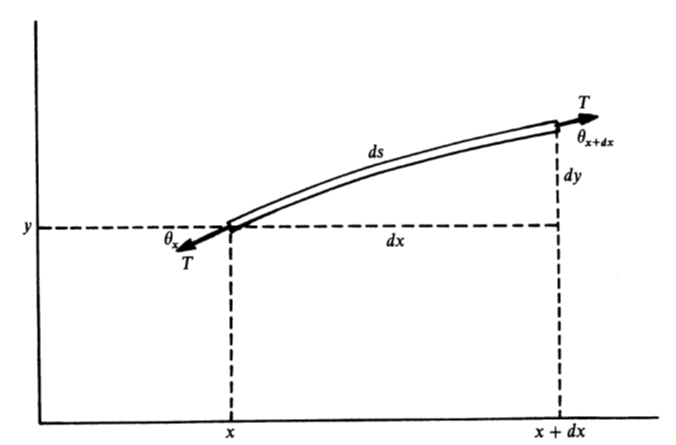
\includegraphics[width=0.6\textwidth]{images/2_10_2.png}
\end{figure}
To describe the behavior of the system, we apply Newton's second law to an infinitesimal segment of the string, extending from \(x\) to \(x + dx\). Due to the perturbation, the string is not perfectly straight, introducing vertical components of tension at the ends of the segment. We assume the perturbation is small, so the angle \(\theta_x\) between the string and the horizontal is small (\( \theta_x \approx \frac{\partial y}{\partial x} \)). 

At the position \(x\), the tension points downwards, while at \(x + dx\), the tension points upwards. The vertical components of the tension are almost the same because the segment length \(dx\) is infinitesimal. However, there is still a small difference, which leads to the net force in the vertical direction. This difference is responsible for the vertical perturbation that propagates as a wave. The net force in the vertical direction is given by:

\[
dF_y = (T \sin \theta)_{x+dx} - (T \sin \theta)_x
\]

Since the variation of tension is infinitesimal, we apply a Taylor expansion \(f(x + dx) = f(x) + \frac{\partial f(x)}{\partial x} dx + \dots\) to approximate the value of \( (T \sin \theta)_{x+dx} \) as:
\[
(T \sin \theta)_{x+dx} = (T \sin \theta)_x + \frac{\partial (T \sin \theta)}{\partial x} dx
\]
The reason we can use these approximations is that for infinitesimal segments, the function can be treated as linear, and the higher-order terms in the Taylor expansion can be neglected.
Substituting this expression into the equation for \(dF_y\), we get:
\[
dF_y = \frac{\partial (T \sin \theta)}{\partial x} dx
\]

For small perturbations, the angle \(\theta\) is small, and we use the approximation \(\sin \theta \approx \theta \approx \frac{\partial y}{\partial x}\). This simplification reduces the expression for \(dF_y\) to:
\[
dF_y = \frac{\partial (T \frac{\partial y}{\partial x})}{\partial x} dx = T \frac{\partial^2 y}{\partial x^2} dx
\]

This result represents the vertical component of the net force acting on the infinitesimal segment. 

According to Newton's second law, the vertical force is also related to the acceleration of the mass of the infinitesimal segment:
\[
dF_y = dm \cdot a_y = \mu ds \frac{\partial^2 y}{\partial t^2}
\]

Here, \(\mu\) is the linear mass density of the string, and \(a_y\) is the vertical acceleration. Equating the two expressions for \(dF_y\), we obtain:
\[
T \frac{\partial^2 y}{\partial x^2} dx = \mu dx \frac{\partial^2 y}{\partial t^2}
\]

Simplifying this, we arrive at the wave equation:
\[
\frac{\partial^2 y}{\partial t^2} = \frac{T}{\mu} \frac{\partial^2 y}{\partial x^2}
\]

The term \(\frac{T}{\mu}\) is the square of the wave propagation velocity, thus, the wave equation becomes:
\[
\frac{\partial^2 y}{\partial t^2} = c^2 \frac{\partial^2 y}{\partial x^2}
\]

This second-order differential equation states that the second derivatives with respect to time and space are proportional. This is precisely the condition for wave propagation. The displacement of the string in the vertical direction propagates along the string as a wave.

The proportionality factor \(c^2 = \frac{T}{\mu}\) shows that the propagation velocity \(c\) depends on the tension \(T\) and the linear mass density \(\mu\) of the string. Higher tension results in faster wave propagation, while higher mass density slows the wave down.  \\

Consider a guitar string, which is fixed at two points. When a perturbation is initiated along the string, it propagates as a wave. The frequency of the sound produced by the string is determined by the time it takes for the wave to travel back and forth along the string, which corresponds to the period (\(T\)).
\[
f = \frac{v}{2L} = \frac{1}{T}
\]
where \(f\) is the frequency of the wave, \(T\) is the tension of the string, \(\mu\) is its linear mass density and \(L\) is its length. As we've seen, for a given string, the wave velocity \(v\) depends on the tension and the linear mass density:
\[
v = \sqrt{\frac{T}{\mu}} \quad \to \quad T = \mu v^2 
\]
Using this, we can determine the tension required to tune the string. 

Let consider two a high E string (\(E_4\)) with the following parameters:
   \[
   f = 329.63 \, \text{Hz}, \quad L = 648 \, \text{mm} = 0.648 \, \text{m}.
   \]
The wave velocity is:
   \[
   v = 2fL = 2 \cdot 329.63 \cdot 0.648 = 427.2 \, \text{m/s}.
   \]

1. For a string with \( \mu = 0.33 \text{g/m} = 0.00033 \, \text{kg/m} \), under the same frequency and length, the tension is:
   \[
   T = \mu v^2 = 0.00033 \cdot (427.2)^2 = 60.2 \, \text{N}.
   \]

2. For a thicker string with \(\mu = 0.39 \, \text{g/m} = 0.00039 \, \text{kg/m}\), under the same frequency and length, the tension is:
   \[
   T = \mu v^2 = 0.00039 \cdot (427.2)^2 = 71.2 \, \text{N}.
   \]

These calculations show that thicker strings (with higher \(\mu\)) require greater tension to achieve the same tuning frequency. This is because the wave velocity must remain constant for a given frequency and string length, necessitating a proportional increase in tension as \(\mu\) increases. The mechanics of a guitar are designed to handle tensions on the order of 60–70 N, corresponding to several kilograms of force. 

Regarding the experience of playing, a heavier string (with higher \(\mu\)) requires greater tension, making it feel stiffer under the fingers when pressed against the fretboard. This tension is the force applied along the length of the string when it is tuned between the bridge and tuning pegs. However, when a string is plucked, the vertical force applied by the musician increases the tension momentarily, altering the string's shape and producing sound. The mechanics of plucking are typically not considered when calculating the resting tension of the string.

Additionally, while the tension depends on \(\mu\), and thus indirectly on the string's diameter (since \(\mu\) is related to the material and cross-sectional area), other factors such as internal forces within the string (e.g., bending and stretching) are often neglected in these idealized calculations. In reality, changes in diameter also affect the string's stiffness and behavior, but these effects are generally minor compared to the dominant influence of \(\mu\) and tension. \\

When analyzing piano strings, we observe that if the tension \(T\) and the linear mass density \(\mu\) are constant, the length of the string \(L\) is expected to vary inversely with the frequency \(f\), i.e., \(L \propto \frac{1}{f}\).
\[
L = \frac{1}{2f} \sqrt{\frac{T}{\mu}}
\]
This relationship also implies that the length of the strings decreases as we move along the piano keys, which explains the tapered shape of a grand piano.
\begin{figure}[H]
    \centering
    \begin{subfigure}[b]{0.3\textwidth}
        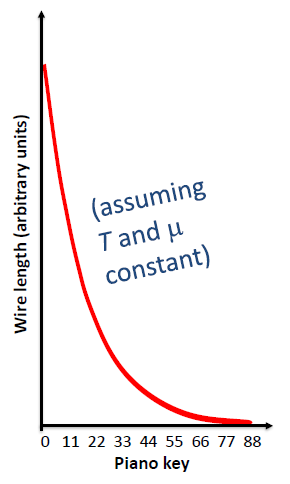
\includegraphics[width=\textwidth]{images/2_13.png}
    \end{subfigure}
    \hfill
    \begin{subfigure}[b]{0.4\textwidth}
        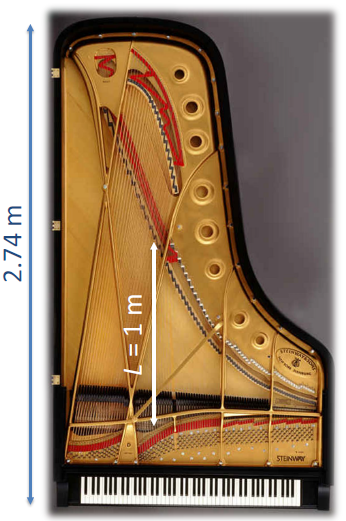
\includegraphics[width=\textwidth]{images/2_14.png}
    \end{subfigure}
\end{figure}
In practice, however, \(T\) and \(\mu\) are not constant for all the strings.The strings are typically made of wound material, consisting of a steel wire core surrounded by a spiral copper wire. To achieve lower frequencies, increasing the mass per unit length \(\mu\) is preferred over reducing the tension \(T\). This adjustment is achieved by increasing the diameter of the string, making it thicker and altering its vibrational behavior (the modes of such strings may no longer be harmonics of the fundamental frequency due to their complexity).

Consider a string of approximate length \(L \approx 1 \, \mathrm{m}\), composed of a steel core and an outer copper winding. The material densities are:\(
\rho_\text{steel} = 7900 \, \mathrm{kg/m^3}, \quad \rho_\text{copper} = 8900 \, \mathrm{kg/m^3}.\)
The diameter of the steel core is \(D_\text{steel} \approx 1 \, \mathrm{mm}\), while the diameter of the copper wire is \(D_\text{copper} \approx 0.5 \, \mathrm{mm}\). The total linear mass density of the string is approximately:
\(
\mu_\text{tot} \approx 27 \, \mathrm{g/m}.
\)\\
We aim to calculate the tension required for the string to produce a sound at a frequency of \(f = 138.6 \, \mathrm{Hz}\), corresponding to the note \(C_3\).

\[
T = \mu v^2, \quad v = 2fL
\]
Substituting:
\[
T = \mu_\text{tot} \cdot (2fL)^2 \approx 1037 \, \mathrm{N}
\]

With 88 keys on a piano and approximately 230 strings, the total tension on the frame exceeds \(15 \, \mathrm{tons}\), which the piano structure must support. This remarkable tension explains the robust construction of grand pianos.


\subsection{Wave Equation Solutions}


Returning to the general wave equation:
\[
\frac{\partial^2 y}{\partial t^2} = v^2 \frac{\partial^2 y}{\partial x^2}
\]
This second-order differential equation has solutions in the form of two functions: one traveling to the right and the other to the left. Mathematically, this is expressed as:
\[
y(x, t) = f_1(x + vt) + f_2(x - vt)
\]

The degrees of freedom in the wave equation are contained within the functions \(f_1\) and \(f_2\), which are determined by the initial conditions. Typically, the initial conditions specify the displacement and velocity of the wave at \(t = 0\):
\[
y(x, 0) = f_1(x) + f_2(x)
\]
\[
\left[\frac{\partial y(x, t)}{\partial t}\right]_{t=0} = v f_1'(x) - v f_2'(x)
\]

When a perturbation starts at a certain location, part of the wave travels to the right, while another part propagates to the left. In an infinite medium, these waves continue indefinitely. However, when we consider a finite string, any discontinuity in the medium—such as the end of the string, a connection to another string, a bridge (e.g., on a guitar), or a change in medium (e.g., air to water)—will cause partial reflection and transmission of the wave. 

Two cases are commonly studied for a string with boundaries:
\begin{itemize}
    \item Fixed end: The string is tied to a rigid surface.
    \item Free end: The string is completely loose and free to move vertically at its end.
\end{itemize}
\begin{figure}[H]
    \centering
    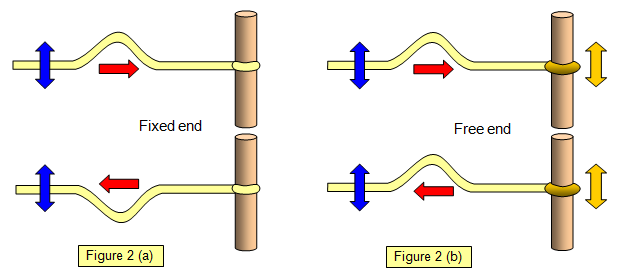
\includegraphics[width=0.7\textwidth]{images/2_16_1.png}
\end{figure}
In the case of a fixed end, the wave is fully reflected, but the reflected wave has the opposite sign (inverted). For a free end, the wave is also fully reflected, but with the same sign (no inversion).

We can analyze this behavior analytically by applying boundary conditions. Initial conditions describe the starting state of the perturbation and determine the form of the wave functions \(f_1(x - vt)\) and \(f_2(x + vt)\). Boundary conditions, on the other hand, describe the constraints imposed by the physical setup of the system.

For example:
\begin{itemize}
    \item At a fixed boundary (e.g., at \(x = 0\)), the vertical displacement of the string must always be zero:
    \[
    y(0, t) = 0 \quad \forall t
    \]
    This ensures that the point of attachment does not move.

    \item At a free boundary (e.g., at \(x = 0\)), there can be no vertical force acting on the string. This means the slope of the string at the boundary must be zero:
    \[
    \left. \frac{\partial y(x, t)}{\partial x} \right|_{x=0} = 0
    \]
    This condition reflects that the string at the boundary is not constrained vertically.
\end{itemize}

In the general solution of the wave equation, we have two functions: one representing a wave moving to the right (\(f_1(x - vt)\)) and the other moving to the left (\(f_2(x + vt)\)). These two waves are part of the mathematical solution, but in a physical system, they represent both the actual wave and the reflected wave. When a perturbation on a finite string reaches a boundary, we can imagine that a "ghost perturbation" originates from the other side of the boundary (outside the string) and enters the system as the reflected wave. In this conceptual model, the physical solution exists on the string, while the mathematical solution extends into the "ghost" region. 

To determine the reflected wave, we apply boundary conditions. These conditions describe how the wave behaves at the boundary of the physical system.

\begin{itemize}
\item Fixed End: At a fixed boundary (e.g., \(x = 0\)), the vertical displacement must always be zero:
   \[
   y(0, t) =  f_1(0 + vt) + f_2(0 - vt) = 0 \quad \forall t
   \]
   Applying this condition, we find that the two functions \(f_1\) and \(f_2\) are the same but have opposite signs:
   \[
   f_1(vt) = -f_2(-vt)
   \]
   This ensures total reflection with inversion of the wave.
   \begin{figure}[H]
    \centering
    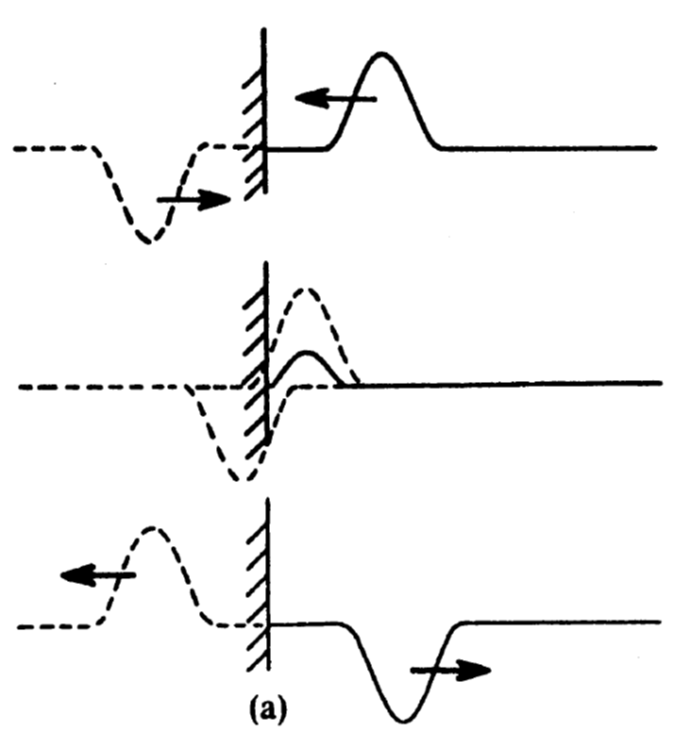
\includegraphics[width=0.3\textwidth]{images/2_17_1.png}
\end{figure}

\item Loose End: At a loose or soft boundary, there can be no vertical force acting on the string. This translates to the condition that the spatial derivative (slope) of the displacement must be zero:
   \[
   \left. \frac{\partial y(x, t)}{\partial x} \right|_{x=0} =  f_1'(0 + vt) + f_2'(0 - vt) = 0
   \]
   Applying this condition, we find that the derivatives of the two functions \(f_1\) and \(f_2\) are equal but with opposite signs:
   \[
   f_1'(vt) = -f_2'(-vt)
   \]
   This ensures total reflection without inversion of the wave.
   \begin{figure}[H]
    \centering
    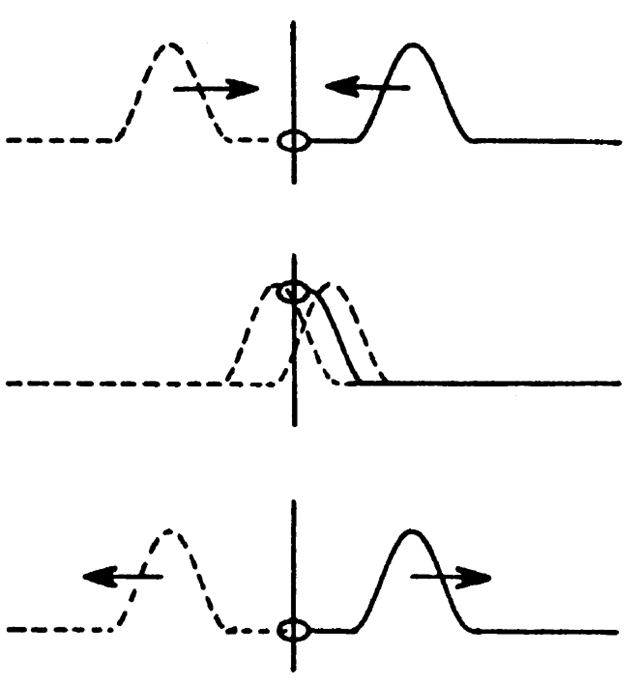
\includegraphics[width=0.3\textwidth]{images/2_17_2.png}
\end{figure}
\end{itemize}
Note: The spatial derivative represents the slope of the string and is not related to the velocity of the wave (given by the temporal derivative).

These conditions demonstrate that reflection is 100\% efficient: the reflected wave carries all the energy of the incoming wave. This is consistent with the mathematical solution, where the boundary conditions dictate the relationships between \(f_1\) and \(f_2\).


\subsection{Wave Equation Harmonic Solutions}

We assume that the \(f\) functions are harmonic functions, which can be expressed using complex exponentials. Harmonic functions serve as valid wave solutions if the argument is \(x - vt\). The general solution is a linear combination of two waves, one moving to the right and one moving to the left:

\[
\Tilde{y}(x, t) = \Tilde{A} e^{j\alpha (x - vt)} + \Tilde{B} e^{j\alpha (x + vt)}
\]

Here, \(\Tilde{A}\) and \(\Tilde{B}\) are the coefficients of the linear combination. The parameter \(\alpha\) ensures the exponent is a pure number, as \(x \pm vt\) represents a length, so \(\alpha\) has units of \(1/\mathrm{m}\).

Introducing the angular frequency \(\omega\) and the wave number \(k\):

\[
\omega = vk, \quad k = \frac{\omega}{v}
\]

Substituting these, we rewrite the solution as:

\[
\Tilde{y}(x, t) = \Tilde{A} e^{j(\omega t - kx)} + \Tilde{B} e^{j(\omega t + kx)}
\]
By reformulating the equation, every variable is associated with an individual coefficient: t is associated with coefficient \(\omega\), whose unit is \(1/\mathrm{s}\), while x is associated with coefficient \(k\), whose unit is \(1/\mathrm{m}\).
The terms \(\omega\) and \(k\) represent oscillation in time and space, respectively:
\begin{itemize}
    \item \(\omega\) is the angular frequency, describing oscillations over time, with \(\omega = 2\pi f\), where \(T = \frac{2\pi}{\omega}\) is the period (time periodicity).
\item \(k\) is the wave number (spatial angular frequency), describing oscillations over space, with \(\lambda = \frac{2\pi}{k}\), the wavelength (spatial periodicity).
\end{itemize}

This symmetry highlights how \(\omega\) governs time oscillations, while \(k\) governs spatial oscillations.

In the context of harmonic waves, we often operate in the complex domain. This allows the coefficients of the linear combination, \(\Tilde{A}\) and \(\Tilde{B}\), to be complex numbers. Each coefficient can therefore be expressed in terms of its amplitude and phase:

\[
\Tilde{A} = A e^{j\phi_A}, \quad \Tilde{B} = B e^{j\phi_B}
\]

Substituting these into the wave equation, we obtain:

\[
\Tilde{y}(x, t) = A e^{j(\omega t - kx + \phi_A)} + B e^{j(\omega t + kx + \phi_B)}
\]

Here \(A\) and \(B\) represent the amplitudes of the two wave components, while \(\phi_A\) and \(\phi_B\) are the initial phases, which define the state of the perturbation at \(t = 0\) and \(x = 0\).

The argument inside the exponential consists of:
\begin{itemize}
\item \(\omega t - kx\) or \(\omega t + kx\): The phase that accumulates over time and space, describing the wave's oscillation.
\item \(\phi_A\) or \(\phi_B\): The initial phase, which characterizes the starting point of the oscillation.
\end{itemize}


This representation highlights that the two components of the wave can have different amplitudes (\(A\), \(B\)) and initial phases (\(\phi_A\), \(\phi_B\)). The overall phase of the wave, therefore, includes contributions from both the oscillatory phase and the initial phase.

To describe the physical displacement of a wave, we focus on the real part of the harmonic solution. For a traveling wave, this can be expressed as:

\[
y(x, t) = \Re\{\Tilde{y}(x, t)\} = A \cos(\omega t - kx + \phi_A) + B \cos(\omega t + kx + \phi_B)
\]

Each harmonic component represents a wave traveling in a specific direction, with its amplitude and initial phase defining its characteristics.

It is important to note that this expression can always be recast into an equivalent form. For instance:

\[
A \cos(\omega t - kx + \phi_A) = A_1 \sin(\omega t - kx) + A_2 \cos(\omega t - kx)
\]

Such transformations allow the harmonic components to be represented as sums of sine and cosine terms. This reformulation is particularly useful when addressing problems involving boundary conditions, such as those encountered in finite strings. In these cases, the sine and cosine decomposition provides a more convenient framework for applying constraints at the boundaries.

The general solution for a harmonic wave can also be written equivalently as:

\[
y(x, t) = A \sin(\omega t - kx) + B \cos(\omega t - kx) + C \sin(\omega t + kx) + D \cos(\omega t + kx)
\]

All these forms describe the same physical solution but provide different perspectives, each suited to specific problem-solving contexts.\\

\subsection{Standing waves}

Now we consider a finite string with fixed ends. At both boundaries, \(x = 0\) and \(x = L\) (the length of the string), the displacement \(y(x, t)\) must be zero at any time. 
\begin{figure}[H]
    \centering
    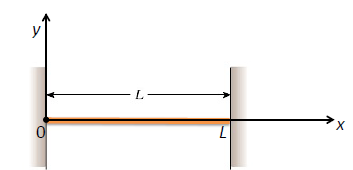
\includegraphics[width=0.5\textwidth]{images/2_20.png}
    \caption{Fixed string}
    \label{fig:2_20}
\end{figure}

This corresponds to the boundary conditions:
\[ y(0, t) = 0, \quad y(L, t) = 0 \]


We start with the general solution for the wave equation:
\[
y(x, t) = A \sin(\omega t - kx) + B \cos(\omega t - kx) + C \sin(\omega t + kx) + D \cos(\omega t + kx).
\]

The first boundary condition, \(y(0, t) = 0\), implies:
\[
y(0, t) = A \sin(\omega t) + B \cos(\omega t) + C \sin(\omega t) + D \cos(\omega t) = 0.
\]

Grouping terms leads to:
\[
(A + C) \sin(\omega t) + (B + D) \cos(\omega t) = 0.
\]

Since this must hold for all times \(t\), the coefficients satisfy:
\[
A = -C, \quad B = -D.
\]

Thus, the general solution reduces to:
\[
y(x, t) = A \sin(\omega t - kx) - A \sin(\omega t + kx) + B \cos(\omega t - kx) - B \cos(\omega t + kx).
\]

The solution can be recast using trigonometric identities:
\[
y(x, t) = [A \sin(\omega t - kx) - A \sin(\omega t + kx)] + [B \cos(\omega t - kx) - B \cos(\omega t + kx)].
\]
Applying the trigonometric subtraction identities:
\[
y(x, t) = 2 [A \cos(\omega t)  - B \sin(\omega t)] \sin(kx).
\]

This representation clearly shows the factor of \(\sin(kx)\), which satisfies the first boundary condition at \(x = 0\).

The second boundary condition, \(y(L, t) = 0\), implies:
\[
y(L, t) = 2 [A \cos(\omega t)  - B \sin(\omega t)] \sin(kL) = 0.
\]

Since this must hold for all times \(t\), we require:
\[
\sin(kL) = 0.
\]

This quantizes the allowed values of \(k\) (harmonic modes on the string):
\[
kL = n\pi, \quad n \in \mathbb{Z}^+.
\]

Thus:
\[
k = \frac{n\pi}{L}, \quad \text{and the angular frequency } \omega_n \text{ satisfies: } \omega_n = vk = \frac{n\pi v}{L}.
\]

The corresponding frequencies of the harmonic modes are:
\[
f_n = \frac{\omega_n}{2\pi} = \frac{nv}{2L}.
\]

This means that only specific wavelengths, \(\lambda_n = \frac{2L}{n}\), associated with frequencies \(f_n = n f_0 = \frac{n v}{2L}\), which are integer multiples of the fundamental frequency \(f_0 = \frac{v}{2L}\), can exist on the string. \\

\textbf{The general solution for the vibration of a finite string} can be expressed as a linear combination of harmonic functions, where each harmonic corresponds to a specific mode determined by the boundary conditions. This is represented mathematically as:

\[
y(x, t) = \sum_n \left[A_n \cos(\omega_n t) + B_n \sin(\omega_n t)\right] \sin\left(\frac{\omega_n}{v} x\right)
\]

Here, \(A_n\) and \(B_n\) are coefficients determined by the initial conditions of the system, such as the initial displacement and velocity of the string. 

If we consider the initial shape of the string (e.g., plucking the string), we can use a Fourier series to expand this initial condition. The Fourier series allows us to decompose the initial shape into a sum of sine functions (harmonics), each with a specific amplitude (Fourier coefficient) corresponding to the harmonic content. 

For example, if the string is plucked at its midpoint, the initial shape is symmetric, resembling a triangle. In this case:

\begin{itemize}
\item The initial triangular shape is even, meaning only harmonics that maintain a maximum at the center (odd harmonics) contribute to the expansion.
\item The first harmonic (fundamental frequency) will have the largest amplitude compared to higher harmonics because it closely matches the overall shape of the initial condition.
\end{itemize}

\begin{figure}[H]
    \centering
    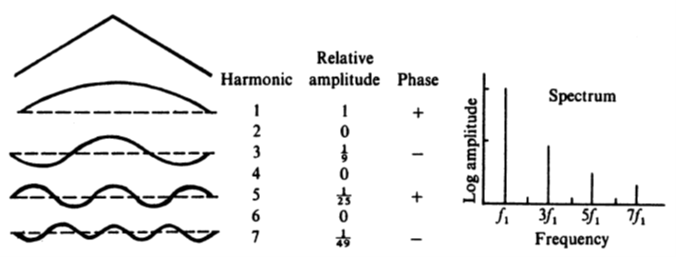
\includegraphics[width=0.7\textwidth]{images/2_22.png}
\end{figure}

If, instead, the string is plucked closer to one end (e.g., near the bridge), the symmetry is broken, and the initial shape no longer resembles the first harmonic. In this case:
\begin{itemize}
\item Higher harmonics contribute more significantly because they align better with the localized maximum.
\item Harmonics with nodes near the plucking position will have negligible contributions since their amplitude is near zero at that location.
\end{itemize}
This harmonic content explains how the sound produced by the string changes depending on the plucking position. When you pluck the string at different points, the resulting harmonic content varies, altering the timbre (or tone quality) of the sound.

Additionally, each harmonic has a phase associated with it. In the context of Fourier series, the phase determines the starting point of the oscillation for each harmonic. When the coefficients are complex (as in the complex domain), the phase can take any value. However, for physical systems with real coefficients, the phase simplifies to either 0 or \(\pi\) (corresponding to a sign change), depending on whether the contribution of a particular harmonic aligns positively or negatively with the initial shape. This alternation of phases ensures that the harmonics combine to accurately reconstruct the sharp edges and overall shape of the initial condition. Harmonics with alternating signs tend to fill the central part of the initial shape, where sharp features like the triangle's peak require contributions from many harmonics.

\subsection{Input Impedance of a String Under External Harmonic Force}

In mechanical systems, an important property is their response to external excitations, which is described by impedance. Impedance relates force and velocity, providing insight into how a system reacts to a given input.\\



Consider an \textbf{infinite string} subjected to an external harmonic force:
\[
\Tilde{f}(t) = F e^{j\omega t}
\]
The general solution for the displacement of the string, assuming a wave traveling to the right, is given by:
\[
\Tilde{y}(x,t) = \Tilde{A} e^{j(\omega t - kx)}
\]
Using Newton's second law, the force per unit length acting on the string is given by:
\[
\Tilde{F} = -T \sin \theta \approx -T \frac{\partial \Tilde{y}}{\partial x}
\]
\begin{figure}[H]
    \centering
    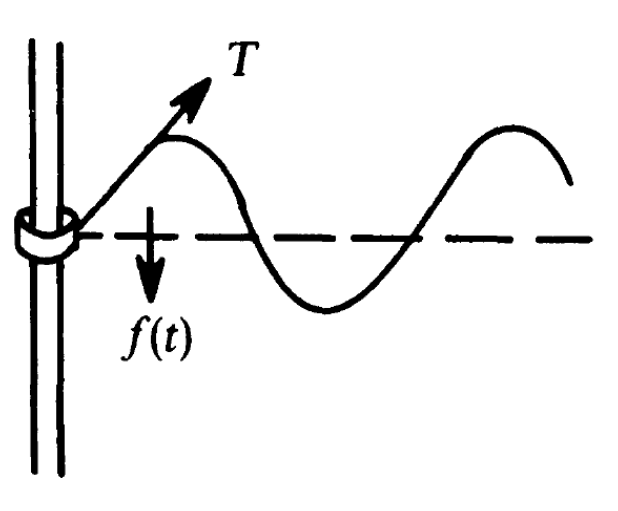
\includegraphics[width=0.3\textwidth]{images/2_23.png}
\end{figure}
Substituting the harmonic forms of \(\Tilde{f}(t)\) and \(\Tilde{y}(x,t)\) into the expression for Newton's second law:
\[
\Tilde{f}(t) = \Tilde{F} \implies F e^{j\omega t} = -T \frac{\partial}{\partial x} \left( \Tilde{A} e^{j(\omega t - kx)} \right)
\quad \text{where} \quad
\frac{\partial \Tilde{y}}{\partial x} = -j k \Tilde{A} e^{j(\omega t - kx)}
\]
Substituting this into the equation gives:
\[
F e^{j\omega t} = j k T \Tilde{A} e^{j\omega t}
\quad \to \quad
\Tilde{A} = \frac{F}{j k T}
\]
Finally, the input or characteristic impedance of the string, which describes the ratio of force to velocity at \(x = 0\), is defined as:
\[
\Tilde{Z}_\text{IN} = Z_0 = \frac{\Tilde{f}(t)}{\Tilde{v}(0,t)}
\]
The velocity at \(x = 0\) is related to the time derivative of \(\Tilde{y}(x,t)\):
\[
\Tilde{v}(0,t) = \frac{\partial \Tilde{y}}{\partial t} \bigg|_{x=0} = j \omega \Tilde{A} e^{j\omega t}
\]
Substituting \(\Tilde{f}(t) = F e^{j\omega t}\) and \(\Tilde{v}(0,t)\) into the impedance formula gives:
\[
Z_0 = \frac{F e^{j\omega t}}{j \omega \Tilde{A} e^{j\omega t}} = \frac{F}{j \omega \Tilde{A}} = \frac{F}{j \omega \frac{F}{j k T}} = k\cdot \frac{T}{\omega} = \frac{\omega}{v} \cdot \frac{T}{\omega} = \frac{\omega}{\sqrt{\frac{T}{\mu}}} \cdot \frac{T}{\omega} = \sqrt{T \mu}
\]
This represents a fundamental property of the string, dependent only on its tension \(T\) and linear mass density \(\mu\).\\




Consider a \textbf{finite string} subject to an external harmonic force:
\[
\Tilde{f}(t) = F e^{j \omega t}
\]
The general solution for the displacement of the string, accounting for waves traveling in both directions (incident wave and reflected wave), is given by:
\[
\Tilde{y}(x,t) = \Tilde{A} e^{j(\omega t - kx)} + \Tilde{B} e^{j(\omega t + kx)}
\]
Using Newton's law, the net force per unit length is:
\[
\Tilde{F} = T (j k \Tilde{A} - j k \Tilde{B}) e^{j \omega t}
\]
Substituting the harmonic force \(\Tilde{f}(t)\):
\[
F e^{j \omega t} = T (j k \Tilde{A} - j k \Tilde{B}) e^{j \omega t}
\]
Boundary conditions at \(x = L\) (fixed end) impose:
\[
0 = \Tilde{A} e^{-j k L} + \Tilde{B} e^{j k L}
\]
Solving this system of equations yields the coefficients:
\[
\Tilde{A} = \frac{F e^{j k L}}{2 j k T \cos(k L)}, \quad \Tilde{B} = \frac{F e^{-j k L}}{-2 j k T \cos(k L)}
\]
The velocity at \(x = 0\) is obtained as the time derivative of \(\Tilde{y}(x, t)\):
\[
\Tilde{v}(0, t) = \frac{\partial \Tilde{y}(0, t)}{\partial t} = j \omega (\Tilde{A} + \Tilde{B}) e^{j \omega t}
\]
Substituting \(\Tilde{A}\) and \(\Tilde{B}\), the input impedance becomes:
\[
\Tilde{Z}_\text{IN} = \frac{\Tilde{f}(t)}{\Tilde{v}(0, t)} = -j Z_0 \cot(k L), \quad
\]

The input impedance has two important properties:
\begin{enumerate}
    \item It is purely imaginary, indicating no energy dissipation. Unlike the infinite string case, where energy carried by the perturbation travels away, in a finite string all energy is reflected back.
    \item The cotangent form implies that the impedance has zeros at specific values of \(kL = n \pi\), where \(n\) is an integer. These values correspond to natural resonant frequencies of the string. In simpler terms, when the frequency of the external force matches one of these natural frequencies (resonances), the string vibrates efficiently in specific patterns called vibrational modes.
\end{enumerate}
\begin{figure}[H]
    \centering
    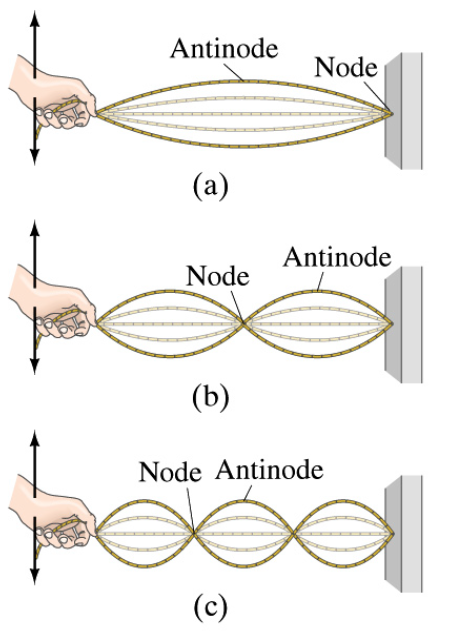
\includegraphics[width=0.3\textwidth]{images/2_24.png}
\end{figure}

\subsection{Impedance Discontinuities}

When a wave traveling along a string encounters a discontinuity, such as a transition between two media with different characteristic impedances, part of the wave is reflected, and part is transmitted. The characteristic impedance of the medium, which depends on the tension \(T\) and the linear mass density \(\mu\), governs the reflection and transmission of the wave.
\begin{figure}[H]
    \centering
    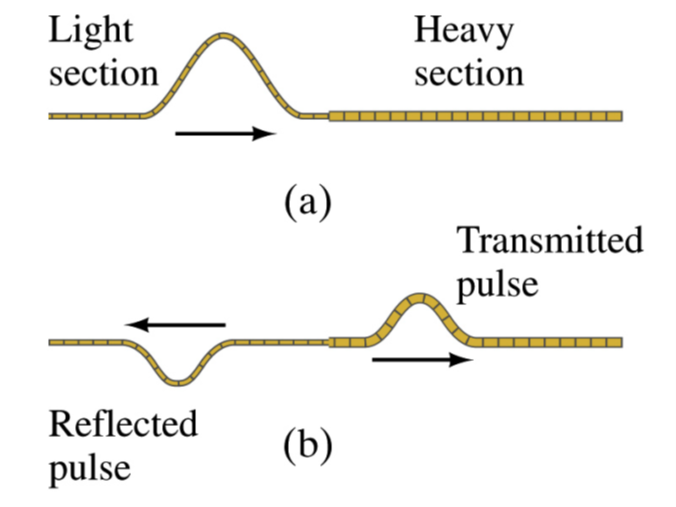
\includegraphics[width=0.5\textwidth]{images/2_25.png}
\end{figure}
At the boundary, the displacement \(\psi(x,t)\) and the restoring force must be continuous:
\[
\begin{aligned}
    &\text{Continuity of displacement: } & \psi_L(0, t) &= \psi_R(0, t) \\
    &\text{Continuity of restoring force: } & T_1 \frac{\partial \psi_L(0, t)}{\partial x} &= T_2 \frac{\partial \psi_R(0, t)}{\partial x}
\end{aligned}
\]

On the left side (\(x < 0\)), the wave is a superposition of the incident wave \(\psi_i\) and the reflected wave \(\psi_r\). On the right side (\(x > 0\)), the wave is only the transmitted wave \(\psi_t\):
\[
\begin{cases}
    \psi_L = \psi_i + \psi_r & x < 0 \\
    \psi_R = \psi_t & x > 0
\end{cases}
\]

By solving the boundary conditions, we obtain the reflection and transmission coefficients, which relate the amplitudes of the reflected and transmitted waves to the amplitude of the incident wave:
\[
\begin{aligned}
    \psi_r &= R \psi_i, \quad R = \frac{Z_1 - Z_2}{Z_1 + Z_2}, \\
    \psi_t &= T \psi_i, \quad T = \frac{2 Z_2}{Z_1 + Z_2}.
\end{aligned}
\]
\begin{itemize}
    \item No Discontinuity (\(Z_1 = Z_2\)):
   If the two media have the same impedance, there is no reflection (\(R = 0\)) and full transmission (\(T = 1\)). This aligns with the physical intuition that a uniform string would allow the wave to pass through without alteration.

\item Low-to-High Impedance Transition (\(Z_1 < Z_2\)):
   In this case, the reflection coefficient \(R\) is negative. The reflected wave has a phase shift of \(\pi\), similar to the case of a rigid boundary. The transmitted wave always maintains the same sign (\(T > 0\)).

\item High-to-Low Impedance Transition (\(Z_1 > Z_2\)):
   The reflection coefficient \(R\) is positive, meaning the reflected wave has no phase shift. The transmitted wave remains positive (\(T > 0\)).
\end{itemize}
For practical systems, such as a string connected to a bridge or a different medium, the reflection and transmission coefficients describe how much of the incident wave energy is reflected and how much is transmitted into the new medium. If the impedance mismatch is large, most of the energy is reflected, whereas for closely matched impedances, most energy is transmitted.

\subsection{Damping in Vibrating Strings}

Let's consider the effects of friction and damping on the oscillation of a vibrating string. While friction is not explicitly included in the standard wave equation, its presence in real systems leads to the decay of oscillations over time. Damping mechanisms for a string can arise from various sources, including:

\begin{itemize}
    \item Medium damping: Friction with the surrounding air, also known as viscous damping, contributes to energy loss as the string oscillates.
    \item Internal damping: Stress within the string material itself (due to imperfections or finite thickness) causes energy dissipation during vibration.
    \item Energy loss through supports: The string is typically attached to supports, such as a bridge on a musical instrument, which are not infinitely rigid. The bridge has a certain impedance, allowing some of the vibrational energy to be transmitted into it and dissipated.
\end{itemize}

These damping effects are often frequency-dependent, meaning their influence on the string’s oscillation varies with the frequency of vibration. In practical scenarios, this damping leads to a gradual reduction in the amplitude of the oscillations over time, affecting the timbre and sustain of the sound produced by the string.

\subsection{Wave Equation in Two Dimensions}

When extending the wave equation to two dimensions, such as describing the behavior of a membrane, the concept of mass density changes from linear mass density to \textit{surface mass density}, denoted as \(\sigma\), with units \([\mathrm{kg/m^2}]\). Similarly, the tension \(T\) is no longer a force but a force per unit length \([\mathrm{N/m}]\).

The two-dimensional wave equation is expressed as:
\[
\frac{\partial^2 f}{\partial t^2} = v^2 \left( \frac{\partial^2 f}{\partial x^2} + \frac{\partial^2 f}{\partial y^2} \right),
\]
where the propagation speed \(v\) is:
\[
v = \sqrt{\frac{T}{\sigma}}.
\]
\begin{figure}[H]
    \centering
    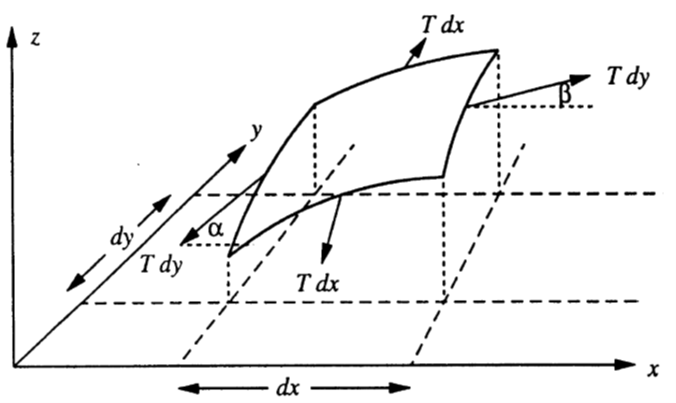
\includegraphics[width=0.5\textwidth]{images/2_27.png}
\end{figure}
For a membrane with fixed edges, the solution of the wave equation involves spatial oscillations along both the \(x\)- and \(y\)-axes. These oscillations are described by two spatial indices, \(m\) and \(n\), which represent the modes of vibration in the \(x\)- and \(y\)-directions, respectively. Each mode is characterized by a combination of these indices.

The general solution for the displacement \(z_{mn}(x, y, t)\) is:
\[
z_{mn}(x, y, t) = \sin\left(\frac{m \pi x}{L_x}\right) \sin\left(\frac{n \pi y}{L_y}\right) \left[M \sin(\omega t) + N \cos(\omega t)\right],
\]
where:
\begin{itemize}
    \item \(L_x\) and \(L_y\) are the dimensions of the membrane along the \(x\)- and \(y\)-directions.
    \item \(m\) and \(n\) are integers representing the number of half-wavelengths along each direction.
    \item \(\omega\) is the angular frequency of the oscillation.
    \item \(M\) and \(N\) are coefficients determined by initial conditions.
\end{itemize}

Each mode is characterized by the pair \((m, n)\), meaning that the membrane can oscillate with different harmonics in the \(x\)- and \(y\)-directions simultaneously. This combination of modes gives rise to complex vibrational patterns, which depend on the boundary conditions and the initial excitation of the membrane.
 

For example, the first-order mode in the \(x\)-direction combined with the first-order mode in the \(y\)-direction is represented as \((m = 1, n = 1)\). In this case, the membrane exhibits a single vibrational mode with only one nodal line, which is along the boundary. In this case, there is one maximum in the center of the membrane, oscillating up and down. The displacement is symmetric with respect to the membrane's center, and the edges remain fixed.

For \(m = 2\) and \(n = 1\), the membrane has two maxima along the \(x\)-axis and one maximum along the \(y\)-axis. This creates nodal lines dividing the membrane into sections where the oscillation occurs out of phase. These nodal lines represent areas where the displacement is zero.
\begin{figure}[H]
    \centering
    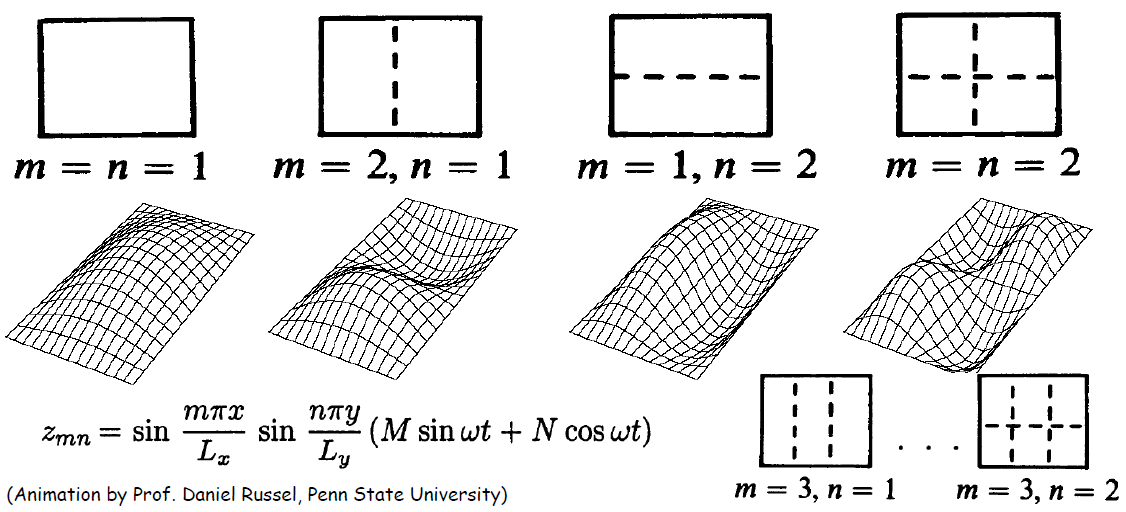
\includegraphics[width=0.6\textwidth]{images/2_28.png}
\end{figure}

For modes \(m = 2, n = 1\) and \(m = 1, n = 2\) on a square membrane, the frequencies of oscillation are identical because the two modes have the same number and arrangement of nodes, due to the symmetry of the membrane. These are called degenerate modes, as they share the same frequency but correspond to distinct vibrational patterns. Degenerate modes are natural vibrational states of the membrane. Any actual oscillation of the membrane is a combination of these modes, described as a linear superposition. The coefficients in this superposition depend on the initial conditions, such as how and where the membrane is disturbed. When degenerate modes are combined, their relative amplitudes and phases influence the final oscillation pattern. This can lead to complex vibration shapes, as the contributions of each mode interact, creating constructive or destructive interference depending on their phases.
\begin{figure}[H]
    \centering
    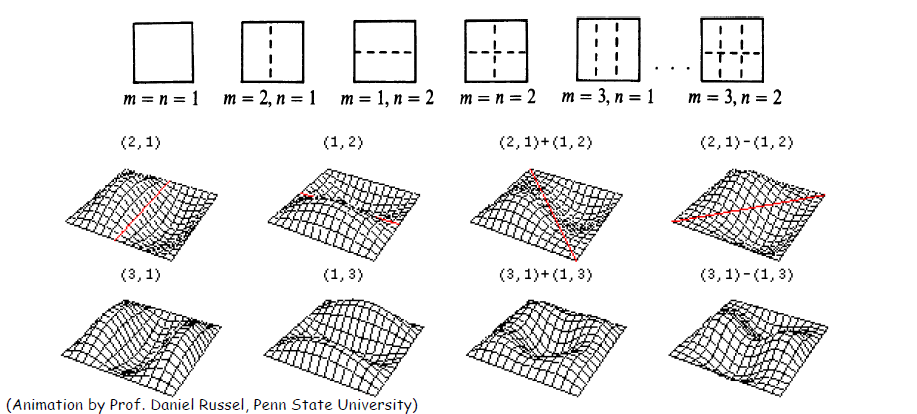
\includegraphics[width=0.7\textwidth]{images/2_29.png}
\end{figure}

If the system is circular, such as a circular membrane, we describe its oscillations using polar coordinates \((r, \theta)\). In this case, the oscillation is two-dimensional, and the vibrational modes are characterized by two indices. These indices define the nature and arrangement of the nodal lines:
\begin{itemize}
    \item Radial nodes: Lines running from the center of the membrane outward, dividing the membrane into sectors.
\item Tangential nodes: Circular lines concentric with the membrane's edge, dividing the membrane into rings.
\end{itemize}
These indices specify the number of radial and tangential nodes in a particular vibrational mode, uniquely identifying each natural oscillation pattern of the circular membrane.
\begin{figure}[H]
    \centering
    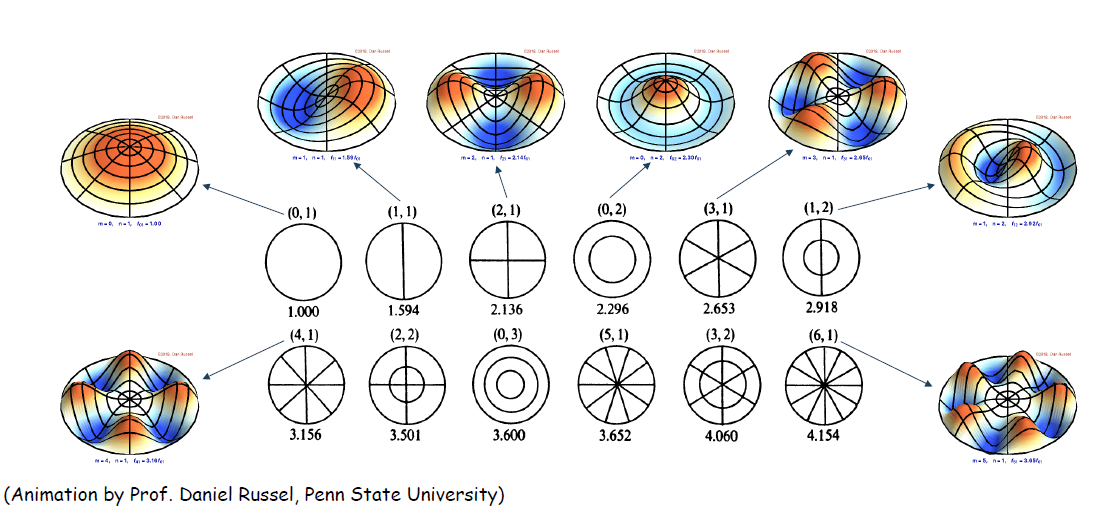
\includegraphics[width=0.9\textwidth]{images/2_30.png}
\end{figure}

In a string, the displacement and velocity are one-dimensional, as the oscillation occurs along a single axis (vertical) while propagating along the length of the string (horizontal). In contrast, a membrane exhibits two-dimensional oscillations, with displacement and velocity varying across both the radial and tangential directions. 

This two-dimensional nature fundamentally alters the behavior of the system. For instance, a cross-sectional view of the membrane's displacement does not resemble that of a string because the oscillations involve complex patterns formed by radial and tangential nodes. 
\begin{figure}[H]
    \centering
    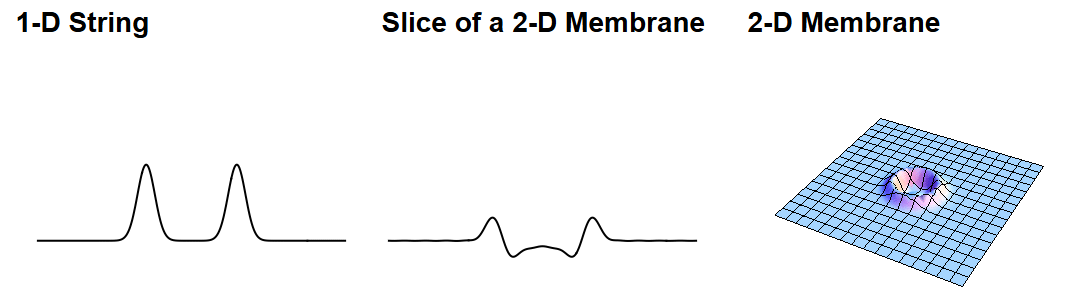
\includegraphics[width=0.8\textwidth]{images/2_31_1.png}
    \caption{Initial Displacement (plucked at the center)}
\end{figure}
\begin{figure}[H]
    \centering
    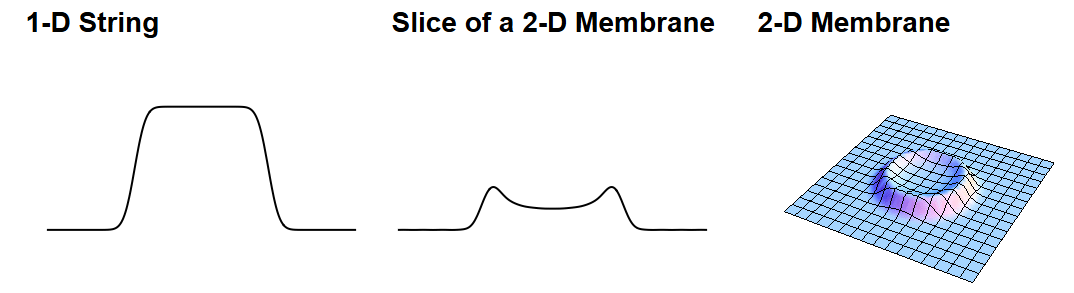
\includegraphics[width=0.8\textwidth]{images/2_31_2.png}
    \caption{Initial Velocity (struck at the center)}
\end{figure}

Strings and membranes are fundamental vibrating systems and serve as primary sources of sound. However, the role of the instrument's body is crucial for amplifying and transforming these mechanical vibrations into powerful sound waves. When a string vibrates, it interacts with the surrounding fluid (air), generating sound waves. On its own, the string's mechanical displacement creates a very weak sound source, barely audible. The majority of the audible sound comes from the transmission of the string's vibrations to another body (e.g., the soundboard of an instrument), which radiates sound waves into the surrounding fluid far more efficiently. Understanding how vibrating systems create waves in a fluid is essential to explain the mechanism of sound production.

\section{Propagation of sounds in fluids}

In the first lecture, we discussed the localized oscillations of masses and springs. The focus was on the displacement and velocity of the mass, without any concept of propagation. In the second lecture, we extended this discussion to include strings and membranes. Here, we introduced the concept of a transverse displacement for each individual element of a string or membrane and the concept of a wave propagates through a medium.

When discussing waves, it is crucial to recognize that there are two distinct types of velocities:
\begin{itemize}
    \item The \textit{displacement velocity} of the mass element (or \textit{mass velocity}), which oscillates due to the wave's influence. 
    \[
\vec{v} = \frac{\partial \vec{s}}{\partial t} \quad \text{where \(\vec{s}\) is the mass displacement} 
\]
    \item The \textit{propagation velocity} of the wave itself (or \textit{wave velocity}), which describes how the wavefront travels through the medium.
\end{itemize}

\subsection{Acoustic Waves in Fluids}

In a fluid, the mass corresponds to each individual molecule, which moves randomly due to thermal motion. If we consider a large number of molecules or observe them over a long period of time, the average displacement and velocity will be zero. Instead of tracking each molecule individually, we consider an infinitesimal volume of the fluid. This approach treats the fluid not as a discrete assembly of molecules but as a continuous medium with a density of molecules. We assume that this infinitesimal volume is small enough to be considered a point in space, yet it contains a sufficiently large number of molecules such that, on average, their random displacements cancel out. This allows us to study the ordered motion of this volume element as it responds to an acoustic wave. 

We now extend our analysis from a one-dimensional string to a three-dimensional fluid space. In this framework, the mass of a given element is described as the volume density of mass, \(\rho\), multiplied by the infinitesimal volume \(dV\). Thus, the infinitesimal mass is given by:
\[
dm = \rho \, dV
\]
(For strings the mass of an infinitesimal element was calculated using the linear mass density, \(\mu\), and the infinitesimal length, \(dx\), as:
\(
dm = \mu \, dx
\)).

This description allows us to discuss both the displacement and the associated velocity of the fluid's mass elements. While in the context of strings and masses, displacement is typically used to describe the motion of waves propagating through the medium, in sound waves, velocity becomes the primary kinematic variable of interest.

(Notice that the mass velocity is represented as a vector quantity, \(\vec{v}\), which depends on the specific system being analyzed. For masses, as in the case of the harmonic oscillator, the velocity is a function of time only: \(\vec{v} = \vec{v}(t)\). For strings, the velocity depends on both position and time: \(\vec{v} = \vec{v}(x, t)\). In the case of fluids, the velocity varies with both the spatial position in three dimensions and time: \(\vec{v} = \vec{v}(\vec{r}, t)\), where \(\vec{r}\) represents the position vector).


\begin{figure}[H]
    \centering
    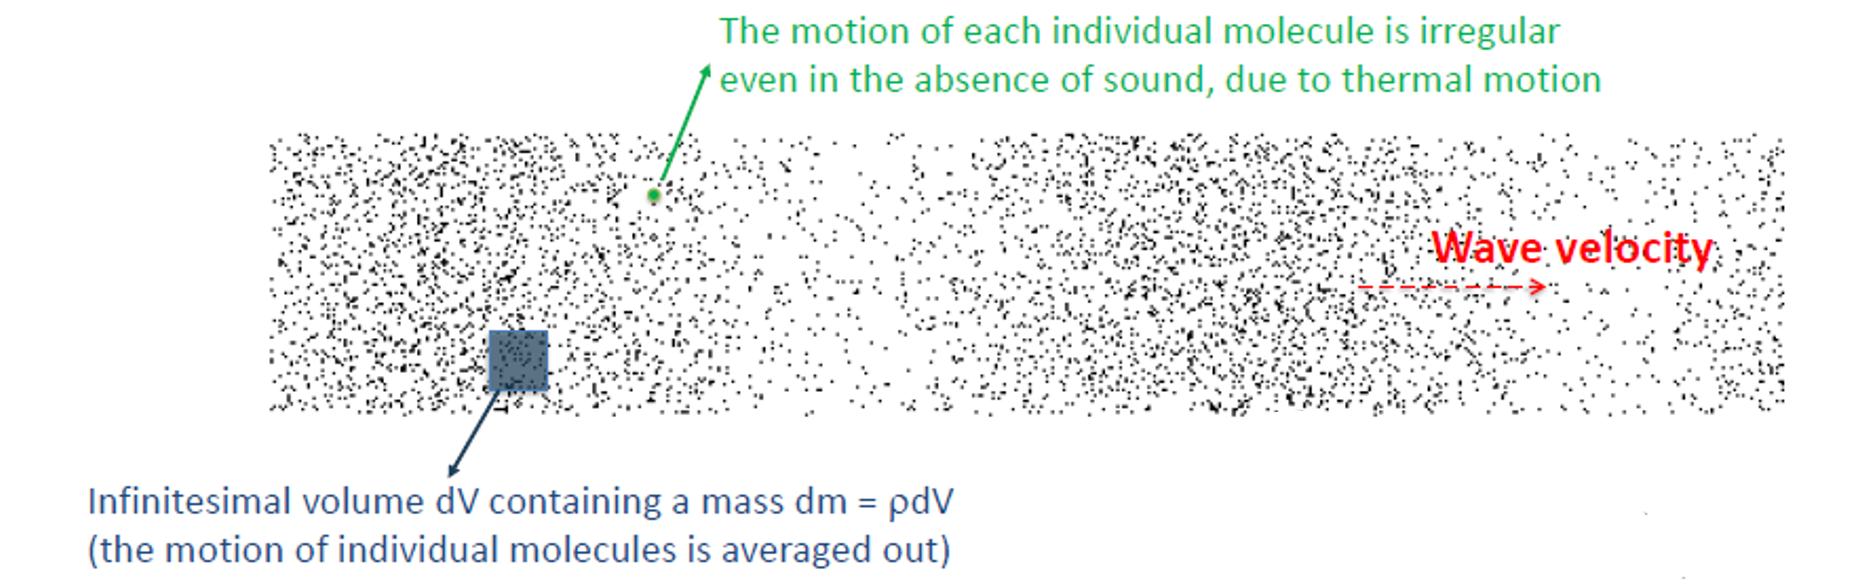
\includegraphics[width=0.9\textwidth]{images/3_3.png}
\end{figure}


Sound wave consists of alternating regions of compression and rarefaction, corresponding to areas of high and low density. To describe this, we associate the local variations in density with these compressions and rarefactions. The total density of the fluid can be expressed as the sum of two terms: 

\[
\rho(\vec{r}, t) = \rho_0(\vec{r}) + \rho_(\vec{r}, t),
\]

where \(\rho_0(\vec{r})\) is the background density of the fluid (i.e., the density in the absence of any sound wave), which, in principle, could depend on spatial position, and \(\rho_(\vec{r}, t)\) is the density perturbation associated with the sound wave, which is a function of both space and time. 

When the density in a specific region is increased or decreased at a given time, the local pressure also varies accordingly. Thus, the total pressure in the fluid is described as:

\[
p(\vec{r}, t) = p_0 + p(\vec{r}, t),
\]

where \(p_0\) is the equilibrium background pressure (e.g., atmospheric pressure), and \(p_(\vec{r}, t)\) represents the pressure perturbation caused by the sound wave. This pressure perturbation can be viewed as a deviation from the equilibrium pressure.

In the propagation of sound waves, the cinematic variable is the velocity, \(\vec{v}\), and the primary physical quantities are density, \(\rho\), and pressure, \(p\). All these quantities—velocity, density, and pressure—are perturbed by the sound wave as it propagates through the medium. Consequently, wave equations can be written to describe the dynamics of each of these quantities, as they all exhibit perturbations in the presence of the acoustic wave.

Pressure in a fluid at equilibrium is a scalar quantity, meaning it does not have a directional component. When measured, it has no dependence on the orientation of the observer. This is true in equilibrium situations (e.g., static air). However, if the fluid is in motion (e.g., water flowing in a river), the situation is not in equilibrium, and directional variations could emerge.

\subsection{Force balance}

Sound waves are created through local compressions and rarefactions, resulting in regions of high and low density. When a region exhibits higher density, it exerts pressure on the surrounding volume, causing molecules in the high-pressure region to impact those in the low-pressure region. This transfers momentum and energy, leading to the propagation of sound waves. To describe this phenomenon mathematically, we rely on Newton's law.

We simplify the problem by considering two variables, space (\(x\)) and time (\(t\)), and assume that the environment is effectively two-dimensional. In this framework, we describe the fluid as a control volume with a certain amount of mass, determined by the surface area, length, and density. The pressure exerted by the outer fluid acts normal to the surfaces of the control volume. At the surface located at \(x\), the pressure is \(p(x, t)\), while at the surface at \(x + dx\), the pressure is \(p(x + dx, t)\). These pressures generate forces that act in opposite directions on the two surfaces. The net force on the control volume arises from the difference between these pressures. If the pressures on both surfaces are equal, the forces cancel out, and no sound wave propagates. However, a sound wave exists when there is a variation in pressure across the control volume, creating a pressure gradient in the environment.
\begin{figure}[H]
    \centering
    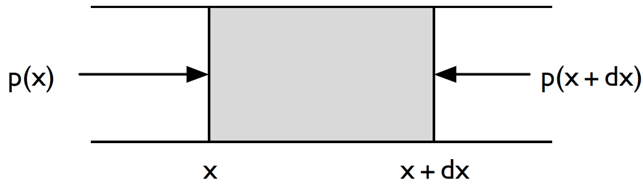
\includegraphics[width=0.6\textwidth]{images/3_5.png}
\end{figure}

For small displacements (\(dx\)), we assume the pressure difference is small and expand it using Taylor's expansion:
\[
p(x + dx, t) = p(x, t) + \frac{\partial p}{\partial x} dx.
\]

The net force is calculated by multiplying the pressure by the surface area \(S\). The force acting at \(x\) has a negative sign, while the force at \(x + dx\) has a positive sign. Substituting the Taylor expansion, the net force in the \(x\)-direction becomes:
\[
dF_x = \left[-p(x + dx, t) + p(x, t)\right]S = -S \frac{\partial p}{\partial x} dx.
\]
The net force arises due to a pressure gradient, represented by the derivative of pressure with respect to \(x\). If the pressure is uniform along \(x\), the gradient \(\frac{\partial p}{\partial x}\) is zero, resulting in no net force and, consequently, no sound wave propagation.
The mass of the control volume is given by:
\[
dm = \rho_\text{TOT} dV = \rho_\text{TOT} S dx,
\]
where \(\rho_\text{TOT}\) is the total density of the fluid.

According to Newton's law, the net force is related to the acceleration of the mass:
\[
dF_x = dm \, a_x = \rho_\text{TOT} S dx \, \frac{dv_x}{dt}
\]
Equating the two expressions for \(dF_x\), we obtain:
\[
-S \frac{\partial p}{\partial x} dx = \rho_\text{TOT} S dx \, \frac{dv_x}{dt}
\quad \to \quad
-\frac{\partial p}{\partial x} = \rho_\text{TOT} \frac{\partial v_x}{\partial t}
\]

The quantities of interest (\(p, v_x, \rho_\text{TOT}\)) depend on both space (\(x\)) and time (\(t\)). However, since \(x\) itself changes with time due to the motion of the fluid within the velocity field, we account for this dependency by calculating the total derivative with respect to time. The total derivative is expressed as:

\[
\frac{df(x(t),t)}{dt} = \frac{\partial f}{\partial t} + \frac{\partial f}{\partial x} \frac{\partial x}{\partial t}.
\]

This formula captures two contributions: the first term, \(\frac{\partial f}{\partial t}\), represents the explicit time variation of the quantity at a fixed position, while the second term, \(\frac{\partial f}{\partial x} \frac{\partial x}{\partial t}\), accounts for changes due to the motion of the point \(x\) in space. If the point \(x\) is stationary (\(\frac{\partial x}{\partial t} = 0\)), the total derivative reduces to the partial derivative with respect to time, reflecting only temporal variations. However, when the fluid moves (\(\frac{\partial x}{\partial t} \neq 0\)), the total derivative includes the contribution from spatial variations carried by the velocity field.


Imagine you are floating in a pond where the water temperature is initially uniform at \(T_0\). As the sun begins to rise, the temperature of the pond increases uniformly over time. If you are stationary and using a thermometer, you would observe a gradual increase in temperature, reflecting the local time variation at your position. This corresponds to the term \(\frac{\partial f}{\partial t}\), representing the change of temperature with time. Now consider a scenario where the sun shines only on one part of the pond, creating a temperature gradient: the water on one side is hotter (\(T_1\)) than the other (\(T_0\)). If you swim from the cooler side (\(T_0\)) to the hotter side (\(T_1\)), your thermometer would still show a change in temperature. However, this change is not due to the passage of time but rather because you are moving through the temperature gradient. This motion corresponds to the term \(\frac{\partial f}{\partial x} \cdot \frac{\partial x}{\partial t}\), where your velocity through the spatial gradient causes the observed variation in temperature. Together, the total change in temperature you experience is the combination of the local time variation (\(\frac{\partial f}{\partial t}\)) and the spatial variation due to your movement (\(\frac{\partial f}{\partial x} \cdot \frac{\partial x}{\partial t}\)).

In the context of sound waves, the function \(f\) represents the velocity field:
\[
\frac{dv_x}{dt} = \frac{\partial v_x}{\partial t} + v_x \frac{\partial v_x}{\partial x}.
\]
Thus, Newton's law for a fluid can be written as:
\[
\mathbf{-\frac{\partial p}{\partial x} = \rho_\text{TOT} \left(\frac{\partial v_x}{\partial t} + v_x \frac{\partial v_x}{\partial x}\right)},
\]
where the net force is driven by the pressure gradient \(-\frac{\partial p}{\partial x}\), and \(\rho_\text{TOT}\) is the total density of the fluid. It is important to note that the velocity \(v_x\) in this equation does not represent the wave's propagation velocity but rather the velocity of the fluid's mass as it responds to the pressure variations caused by the sound wave.

Finally, this formulation provides the first of three equations necessary to describe the propagation of sound waves. 


\subsection{Mass Balance}

The principle of mass conservation states that the total mass in a system must remain constant. Specifically, a change in density, which is associated with a change in pressure, cannot arise spontaneously. If mass appears or disappears within a given volume, it must originate from or flow to the surrounding environment. 
\begin{figure}[H]
    \centering
    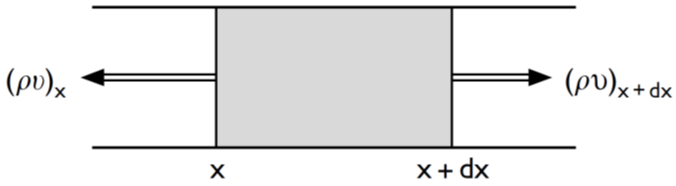
\includegraphics[width=0.6\textwidth]{images/3_6.png}
\end{figure}
To quantify this, we calculate the flux of mass entering and exiting the control volume through its boundaries at \(x\) and \(x + dx\). Consider a surface of area \(S\) through which particles, with a mass density \(\rho_\text{TOT}(x, t)\), move at a velocity \(v_x(x, t)\). The total mass of particles crossing this surface in a time interval \(dt\) is given by:  
\[
dm = \rho_\text{TOT}(x,t) v_x(x,t) S dt.
\]  
Here, \(v_x(x,t) \, dt\) represents the maximum distance that particles can travel from the surface to cross it within the time interval \(dt\).

From this, the mass flux (the mass flowing through the surface per unit time) can be expressed as:  
\[
\frac{dm}{dt} = \rho_\text{TOT}(x,t) v_x(x,t) S.
\]  

Since both the density and velocity are functions of position and time, the flux differs at \(x\) and \(x + dx\). By applying a Taylor expansion, we determine the net flow through the boundaries of the volume:
\begin{align*}
    \left[\rho_\text{TOT} v_x(x, t) - \rho_\text{TOT} v_x(x + dx, t)\right]S 
    &= \left[\rho_\text{TOT}(x, t) v_x(x, t) - \left(\rho_\text{TOT}(x, t) v_x(x, t) + \frac{\partial (\rho_\text{TOT} v_x)}{\partial x} dx \right)\right] S \\
    &= -S \frac{\partial (\rho_\text{TOT} v_x)}{\partial x} dx.
\end{align*}

The net flow results in a mass change ( \(\frac{dm}{dt}\)) within the volume \(Sdx\), leading to a change in density ( \(\frac{d\rho}{dt}\)). This relationship is given by:
\[
- \frac{\partial (\rho_\text{TOT} v_x)}{\partial x} S dx = \frac{\partial \rho}{\partial t} S dx.
\]

Simplifying, we find the second equation:
\[
\mathbf{\frac{\partial \rho}{\partial t} + v_x \frac{\partial \rho_\text{TOT}}{\partial x} + \rho_\text{TOT} \frac{\partial v_x}{\partial x} = 0.}
\]
Where the term \(\frac{\partial (\rho_\text{TOT} v_x)}{\partial x}\) is expanded using the product rule:
   \(
   \frac{\partial (\rho_\text{TOT} v_x)}{\partial x} = \frac{\partial \rho_\text{TOT}}{\partial x} v_x + \rho_\text{TOT} \frac{\partial v_x}{\partial x}.
   \)
This equation demonstrates that the change in density is directly related to the net flux of mass through the volume's boundaries. It complements the first equation, which describes the forces acting on the system and the resulting acceleration. Together, these two equations provide a comprehensive model of the dynamics of the fluid medium in response to sound wave propagation.

\subsection{Equation of State}
The equation of state arises from thermodynamic principles, where density (\(\rho_\text{TOT}\)), pressure (\(p_\text{TOT}\)), and temperature (\(T\)) are interrelated. From thermal physics, we know that these quantities are not independent, and their relationship is captured by an equation of state. For instance, in the case of an ideal gas, the equation of state is given by:

\[
pV = nRT,
\]

where \(n/V\) represents the mass density. In general, for real gases or fluids, the state variables obey the functional relationship:

\[
f(\rho_\text{TOT}, p_\text{TOT}, T) = 0.
\]

For adiabatic processes, where there is no heat exchange with the surroundings, we can simplify this equation. In particular, under the assumption of adiabatic expansion or compression of the fluid, temperature \(T\) becomes less relevant, and we directly relate pressure and density:

\[
\mathbf{p_\text{TOT} = p_\text{TOT}(\rho_\text{TOT})}.
\]

The assumption of adiabaticity is justified by considering the frequency of sound waves. Sound waves oscillate rapidly, and their characteristic timescales are much shorter than the timescales for heat exchange with the surroundings. This implies that during the compression and expansion cycles of the wave, heat transfer can be neglected.

With this third equation—the equation of state—we complete the description of the problem. Together with the force balance (Newton's law) and the mass balance equations, we have a comprehensive framework for analyzing wave propagation in the fluid, without any further simplifications, apart from the adiabatic assumption.

\[
\begin{cases}
-\frac{\partial p}{\partial x} = \rho_\text{TOT} \left( \frac{\partial v_x}{\partial t} + v_x \frac{\partial v_x}{\partial x} \right) & \text{(1)} \\
v_x \frac{\partial \rho_\text{TOT}}{\partial x} - \rho_\text{TOT} \frac{\partial v_x}{\partial x} = \frac{\partial \rho}{\partial t} & \text{(2)} \\
p_\text{TOT} = p_\text{TOT}(\rho_\text{TOT}) & \text{(3)}
\end{cases}
\]



\subsection{Linear wave equation}

To solve the system analytically, we introduce approximations that are valid under standard conditions of sound propagation, such as speech or music. However, these assumptions break down under extreme conditions of pressure waves.

First, we assume that the \textit{changes in density and pressure caused by the sound wave are much smaller than the background density \(\rho_0(x)\) and pressure} \(p_0(x)\):
\[
\begin{cases}
\rho(x, t) \ll \rho_0(x) \\
p(x, t) \ll p_0(x)
\end{cases}
\]
This implies that sound represents a very small perturbation of the initial conditions. While this is a reasonable mathematical approximation, it also highlights the extraordinary sensitivity of the human ear, capable of perceiving such tiny variations.

Additionally, we assume \textit{small velocities}, such that:
\[
v_x \approx 0,
\]
although we do not neglect the derivatives of velocity. 

Another crucial assumption is a linear relation between pressure and density, also known as \textit{linear equation of state}:
\[
p = c^2 \rho,
\]
where \(c^2\) is the proportionality constant, valid for low sound levels.

By applying these approximations, we simplify the governing equations into a system of two symmetrical equations relating pressure and velocity:
\begin{equation}
\label{eq:acoustic_wave_equations}
\begin{cases}
\frac{\partial p}{\partial x} = -\rho_0 \frac{\partial v_x}{\partial t} \\
\rho_0 \frac{\partial v_x}{\partial x} = -\frac{1}{c^2} \frac{\partial p}{\partial t}
\end{cases}
\end{equation}

To eliminate \(v_x\), we differentiate the first equation with respect to \(x\) and the second equation with respect to \(t\):
\[
\mathbf{\frac{\partial^2 p}{\partial x^2} = \frac{1}{c^2} \frac{\partial^2 p}{\partial t^2}}.
\]
This shows that pressure, under the small perturbation approximation, satisfies the wave equation. The proportionality constant \(1/c^2\) indicates that the wave propagates with velocity \(c\), which is also the proportionality factor between pressure and density.

Similarly, by differentiating appropriately, we can derive wave equations for \(v_x\) and \(\rho\). From the second equation, we find:
\[
\frac{\partial^2 v_x}{\partial x^2} = \frac{1}{c^2} \frac{\partial^2 v_x}{\partial t^2}.
\]
The same approach can be used to derive a wave equation for density \(\rho\), completing the description of the system.


\subsection{3D Sound Waves in Fluid}

We extend these equations from a single spatial dimension, where the position variable is scalar, to three dimensions, where the position becomes a vector. This allows us to write each equation for all Cartesian directions, accounting for the behavior of the system.
\[
\begin{cases}
\frac{\partial p}{\partial x} = -\rho_0 \frac{\partial v_x}{\partial t} & \rightarrow
\begin{cases}
\frac{\partial p}{\partial x} = -\rho_0 \frac{\partial v_x}{\partial t} \\
\frac{\partial p}{\partial y} = -\rho_0 \frac{\partial v_y}{\partial t} \\
\frac{\partial p}{\partial z} = -\rho_0 \frac{\partial v_z}{\partial t}
\end{cases} \\[10pt]
\rho_0 \frac{\partial v_x}{\partial x} = -\frac{1}{c^2} \frac{\partial p}{\partial t} & \rightarrow
\rho_0 \left( \frac{\partial v_x}{\partial x} + \frac{\partial v_y}{\partial y} + \frac{\partial v_z}{\partial z} \right) = -\frac{1}{c^2} \frac{\partial p}{\partial t}
\end{cases}
\]

To achieve this, we introduce the velocity vector \(\vec{v}\) and the Nabla operator \(\nabla\), which is defined as a vector containing the three spatial partial derivatives:

\[
\vec{\nabla} = \frac{\partial}{\partial x} \hat{u}_x + \frac{\partial}{\partial y} \hat{u}_y + \frac{\partial}{\partial z} \hat{u}_z
\]

When the \(\nabla\) operator acts on a scalar field, such as pressure \(p\), it produces the gradient of \(p\), which is a vector indicating the direction of maximum change in \(p\) and whose magnitude is the rate of change along that direction:

\[
\nabla p = \frac{\partial p}{\partial x} \hat{u}_x + \frac{\partial p}{\partial y} \hat{u}_y + \frac{\partial p}{\partial z} \hat{u}_z.
\]

For longitudinal waves, such as sound waves, the molecular oscillations and the fluid displacement occur along the propagation direction. Therefore, the velocity vector \(\vec{v}\) aligns with the propagation direction. This alignment implies that any changes in \(\vec{v}\), such as its time derivative, must also point in the same direction. Consequently, the gradient of pressure \(\nabla p\) identifies the direction in which the wave propagates, as it aligns with the maximum pressure variation.

\[
\begin{cases}
\frac{\partial p}{\partial x} = -\rho_0 \frac{\partial v_x}{\partial t} \\
\frac{\partial p}{\partial y} = -\rho_0 \frac{\partial v_y}{\partial t} \\
\frac{\partial p}{\partial z} = -\rho_0 \frac{\partial v_z}{\partial t}
\end{cases}
\quad \to \quad
\vec{\nabla} p = -\rho_0 \frac{\partial \vec{v}}{\partial t}
\]




The second equation involves the flow of mass along the three directions. When the \(\nabla\) operator acts on a vector field, such as \(\vec{v}\), we compute the divergence:

\[
\nabla \cdot \vec{v} = \frac{\partial v_x}{\partial x} + \frac{\partial v_y}{\partial y} + \frac{\partial v_z}{\partial z}.
\]

This divergence quantifies the rate at which the fluid's velocity field spreads out or contracts, indicating the net mass flow in a given region.

\[
\rho_0 \left( \frac{\partial v_x}{\partial x} + \frac{\partial v_y}{\partial y} + \frac{\partial v_z}{\partial z} \right) = -\frac{1}{c^2} \frac{\partial p}{\partial t}
\quad \to \quad
\rho_0 \vec{\nabla} \cdot \vec{v} = -\frac{1}{c^2} \frac{\partial p}{\partial t}
\]


By writing the equations of motion and continuity in terms of the \(\nabla\) operator, we obtain a compact vectorial formulation of the governing equations. 
\begin{equation}
\label{eq:acoustic_wave_equations_3D}
\begin{cases}
\vec{\nabla} p = -\rho_0 \frac{\partial \vec{v}}{\partial t} \\
\rho_0 \vec{\nabla} \cdot \vec{v} = -\frac{1}{c^2} \frac{\partial p}{\partial t}
\end{cases}
\end{equation}
Applying the \(\nabla\) operator to the first equation and taking the time derivative of the second equation allows us to combine them. This results in a wave equation for the pressure field in three dimensions:

\[
\nabla^2 p = \frac{1}{c^2} \frac{\partial^2 p}{\partial t^2},
\]

where \(\nabla^2\) is the Laplacian operator:

\[
\nabla^2 = \frac{\partial^2}{\partial x^2} + \frac{\partial^2}{\partial y^2} + \frac{\partial^2}{\partial z^2}.
\]

This final equation is coordinate-independent, making it valid in any coordinate system. However, the expression for the \(\nabla\) operator must be adapted to the chosen coordinate system, such as cylindrical or spherical coordinates.


\subsection{Plane Waves}

If we observe the propagation direction along the \(x\)-axis and take a snapshot at a given time, all the variables (such as pressure and velocity) will be uniform over planes perpendicular to the \(x\)-axis. This setup allows us to analyze plane waves—those waves whose wavefronts are planes. These waves can be described by the 1D wave equation, provided that the coordinate axis aligns with the direction of wave propagation.
\begin{figure}[H]
    \centering
    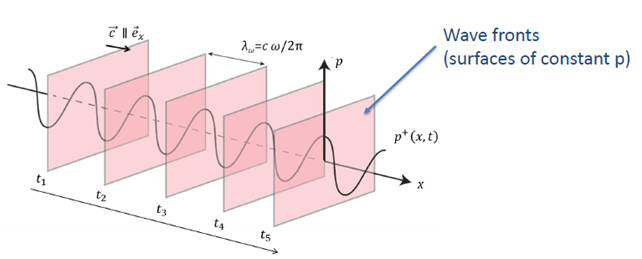
\includegraphics[width=0.8\textwidth]{images/3_10.png}
\end{figure}
The general solution of the wave equation is a combination of forward and backward propagating waves. The coefficients are generally complex numbers and can be expressed using exponential notation. This leads to the following mathematical representation of the pressure wave:

\[
\tilde{p}(x, t) = \tilde{A} e^{j(\omega t - kx)} + \tilde{B} e^{j(\omega t + kx)} = A e^{j(\omega t - kx + \phi_A)} + B e^{j(\omega t + kx + \phi_B)}.
\]

Here, \(\omega\) is the angular frequency, \(k\) is the wavenumber, \(\phi_A\) and \(\phi_B\) are the initial phases, and \(A\) and \(B\) are amplitudes. To retrieve the physical, real part of this solution, we take the real part of \(\tilde{p}(x, t)\):

\[
p(x, t) = \Re[\tilde{p}(x, t)] = A \cos(\omega t - kx + \phi_A) + B \cos(\omega t + kx + \phi_B).
\]

This can be further expanded into sine and cosine terms:

\[
p(x, t) = A \sin(\omega t - kx) + B \cos(\omega t - kx) + C \sin(\omega t + kx) + D \cos(\omega t + kx).
\]

The argument of the oscillatory function (here, of the complex exponential) is referred to as the phase of the wave. It depends on time (\(\omega t\)), space (\(kx\)), and the initial phase (\(\phi\)). 

Wavefronts are defined as locations where the phase is constant at a certain time. Setting the phase equal to a constant \(C\), we get:

\[
\omega t - kx + \phi = C. \quad \to \quad x = \frac{\omega t + \phi - C}{k}.
\]

this describes planes perpendicular to the direction of propagation. These are planes of constant pressure and phase.

As time progresses, each wavefront moves forward with the wave's propagation velocity \(c\). The distance between two wavefronts of the same pressure and phase corresponds to the wavelength \(\lambda\). 

While real sound waves are not infinitely extended plane waves, this concept is useful for approximations. For example, a loudspeaker emits spherical waves due to its localized source, but when these waves reach our ears (small compared to the wavelength), they can be locally approximated as plane waves.

\subsection{Impedance in Plane Wave}

When analyzing the oscillations of mass-spring systems or wave propagation along strings, we introduced the concept of impedance, which quantifies the system's response to a stimulus. For mass-spring systems and strings, impedance relates force and velocity. In the context of plane waves in fluids, we use pressure instead of force, and impedance is calculated as the ratio of pressure to velocity.

To calculate the impedance of wave propagation in a fluid, we first determine the velocity \(v_x\). Considering the equation \ref{eq:acoustic_wave_equations}:
\[
v_x = -\frac{1}{\rho_0} \int \frac{\partial p}{\partial x} dt.
\]

Substituting the expressions for the pressure components, we derive:
\[
v_x = \frac{1}{\rho_0 c} \left[\tilde{p}^+(x,t) - \tilde{p}^-(x,t)\right] = \frac{1}{Z_0} \left[\tilde{p}^+(x,t) - \tilde{p}^-(x,t)\right],
\]
where:
\[
\tilde{p}^+(x,t) = {\tilde A} e^{j(\omega t - kx)}, \quad \tilde{p}^-(x,t) = {\tilde B} e^{j(\omega t + kx)}.
\]

Here, \(Z_0 = \rho_0 c\) is the characteristic impedance of the medium, where \(\rho_0\) is the equilibrium density of the medium and \(c\) is the speed of sound in the medium. The forward wave (\(p^+\)) and backward wave (\(p^-\)) have associated impedances \(Z^+ = Z_0\) and \(Z^- = -Z_0\), respectively. The difference in sign is a convention reflecting the direction of propagation.

The impedance for plane wave propagation in a fluid is a real number, indicating a direct proportionality between pressure and velocity, but only for a single wave. If we consider only the forward-propagating wave (\(p^+\)), the pressure and velocity are directly proportional. Similarly, for the backward-propagating wave (\(p^-\)), the proportionality holds. However, when both forward and backward waves are present, this direct proportionality no longer applies, as the two waves have different impedances and opposite signs.

\subsection{Plane Waves with Arbitrary Orientation}

To describe plane waves that do not align with any specific reference axis, we generalize the 1D scalar formulation into a vectorial formulation. This occurs when the wave propagates in a direction that cannot be conveniently oriented along one of the axes in our coordinate system, for instance, when reflections or other interactions occur.
\begin{figure}[H]
    \centering
    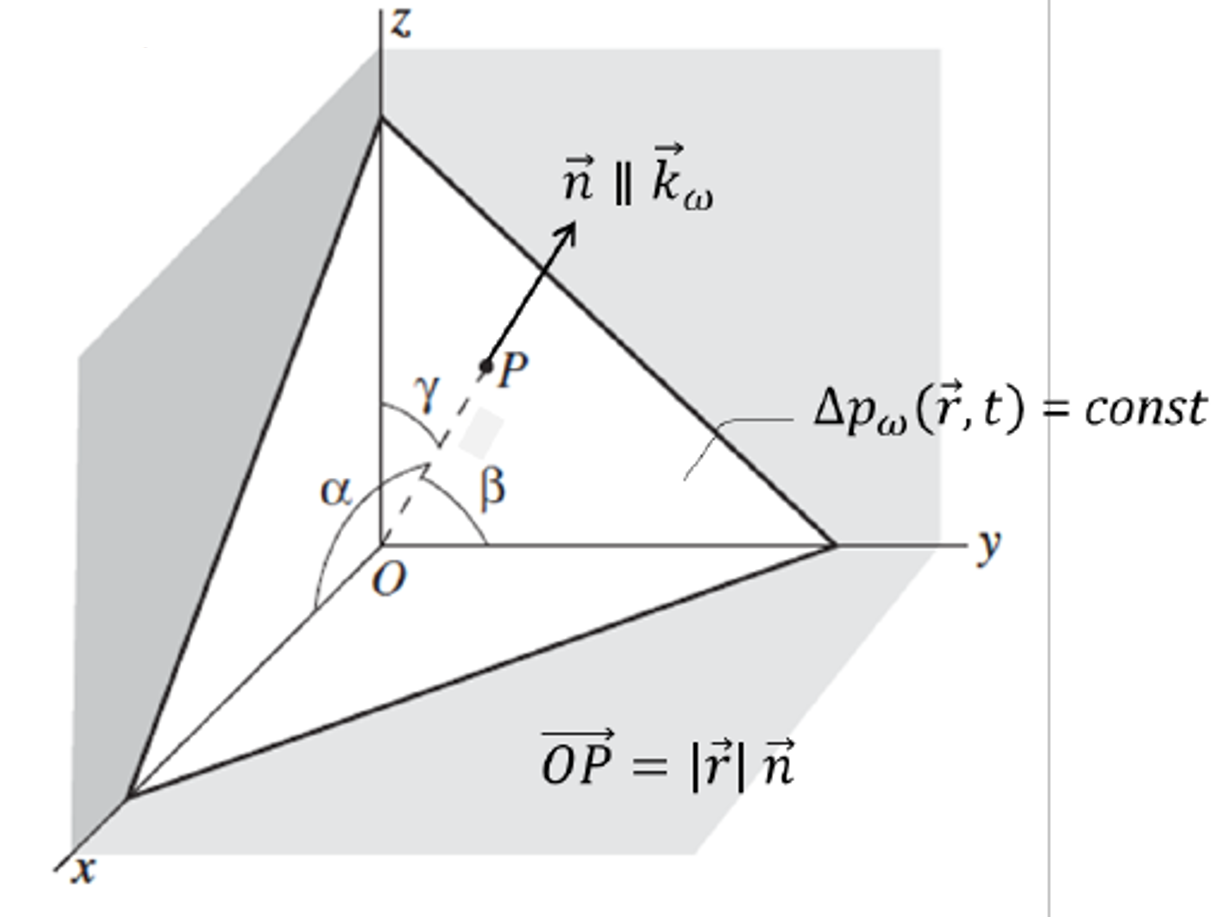
\includegraphics[width=0.5\textwidth]{images/3_12.png}
\end{figure}

In this vectorial representation:
\begin{itemize}
    \item  The wavevector \(\vec{k}\) is introduced. It points along the direction of wave propagation, which is also normal to the wavefront planes. For a scalar 1D problem, the propagation was aligned with the \(x\)-axis, , and thus \(\vec{k}\) had only one component \(k_x\), but now we allow the propagation direction to be arbitrary in space.
    The vector \(\vec{k}\) can be decomposed into components along the \(x\)-, \(y\)-, and \(z\)-axes as:
\[
\vec{k} = k_x \hat{u}_x + k_y \hat{u}_y + k_z \hat{u}_z = k \left[\cos\alpha \hat{u}_x + \cos\beta \hat{u}_y + \cos\gamma \hat{u}_z\right],
\]
where \(\cos\alpha\), \(\cos\beta\), and \(\cos\gamma\) are the direction cosines of \(\vec{k}\) with respect to the coordinate axes.

\item The equation of the wavefronts transitions from \(kx = \text{const}\) in 1D to \(\vec{k} \cdot \vec{r} = \text{const}\) in the generalized case. Here, \(\vec{r}\) is the position vector describing the location in 3D space. This equation still describes planes normal to the propagation direction (\(\vec{k}\)), but the propagation direction is no longer constrained to align with any particular axis.
\end{itemize}



For a position vector \(\vec{r} = x\hat{u}_x + y\hat{u}_y + z\hat{u}_z\), the wave solution becomes:
\[
\tilde{y}(\vec{r}, t) = \tilde{A} e^{j(\omega t - \vec{k} \cdot \vec{r})} + \tilde{B} e^{j(\omega t + \vec{k} \cdot \vec{r})}.
\]
This equation describes a plane wave in 3D, where the phase depends on both time \(t\) and position \(\vec{r}\), and the wavefronts are planes perpendicular to the wavevector \(\vec{k}\).

\subsection{Sound Velocity}



In the context of acoustic waves, small changes in pressure lead to small changes in density, allowing a linear approximation of their relationship. The total density \(\rho_\text{TOT}\) is expressed as the sum of the equilibrium density \(\rho_0\) and the perturbation density \(\rho\): 

\[
\rho_\text{TOT} = \rho_0 + \rho.
\]

Assuming a dependence of \(\rho_\text{TOT}\) on the total pressure \(p_\text{TOT}\), we use a Taylor expansion around the equilibrium pressure \(p_0\) for small perturbations:

\[
\rho_\text{TOT}(p_\text{TOT}) \approx \rho_0 + \left(\frac{\partial \rho}{\partial p}\right)_0 (p_\text{TOT} - p_0),
\]

where \(\rho_\text{TOT}(p_0) = \rho_0\) and \(p_\text{TOT} - p_0 = p\). Simplifying:

\[
\rho_\text{TOT} = \rho_0 + \left(\frac{\partial \rho}{\partial p}\right)_0 p.
\]

Thus, the perturbation density is:

\[
\rho = \rho_\text{TOT} - \rho_0 = \left(\frac{\partial \rho}{\partial p}\right)_0^{(\text{ad})} p,
\]


where \(\left(\frac{\partial \rho}{\partial p}\right)_0^{(\text{ad})}\) is the derivative of density with respect to pressure calculated along an adiabatic path. This describes how much the density increases for a given pressure change in an isentropic (adiabatic and reversible) process.


The isentropic compressibility coefficient, \(\beta_\text{ad}\), quantifies the relationship between pressure and density:

\[
\beta_\text{ad} = \frac{1}{\rho_0} \left(\frac{\partial \rho}{\partial p}\right)_0^{(\text{ad})}.
\]

The bulk modulus, \(K_\text{ad}\), is defined as the reciprocal of the compressibility:

\[
K_\text{ad} = \frac{1}{\beta_\text{ad}}.
\]

Using these relationships, the proportionality between pressure and density is given by:

\[
p = \frac{K_\text{ad}}{\rho_0} \rho = c^2 \rho,
\]

where \(c\) is the speed of sound in the medium:

\[
c = \sqrt{\frac{K_\text{ad}}{\rho_0}}.
\]

This equation provides a clear link between the thermodynamic properties of the medium (through \(K_\text{ad}\) and \(\rho_0\)) and the propagation speed of sound waves. It validates the proportionality factor \(c^2\), which was previously assumed in the linearized wave equation. \\


In the context of adiabatic transformations, where no heat exchange occurs between the system and its surroundings, the pressure and volume of an ideal gas change as \(p V^\gamma = \text{constant}\), where \(\gamma\) is the ratio of specific heats at costant pressure and volume:
\[ \gamma = \frac{C_p}{C_v}
\]

For an ideal gas, the state equation can be written in terms of:
   \(
   p V = n R T,
   \)
   where:\(n\) is the number of moles,\(R\) is the universal gas constant, \(T\) is the temperature.  Alternatively, using mass \(m\) instead of \(n\), we express it as:
   \(
   p V = m R^* T,
   \)
   where \(R^* = \frac{R}{M}\) is the specific gas constant (with \(M\) being the molar mass).  
Dividing by \(V\), we can write the ideal gas law in terms of density \(\rho\) as:
   \(
   p = \rho R T.
   \)
Recasting the adiabatic equation \(p V^\gamma = \text{constant}\) using density, we find:
   \(
   p \rho^{\gamma} = \text{constant}.
   \). This shows that during adiabatic transformations, pressure and density remain proportional in a specific manner:
   \[
   \ p_0 \rho_0^\gamma = \ p \rho^\gamma 
   \quad \to \quad
   \frac{p}{p_0} = \left(\frac{\rho}{\rho_0}\right)^\gamma,
   \]
   where \(p_0\) and \(\rho_0\) are the initial pressure and density, respectively.


From this, we can express the density as a function of pressure:

\[
\rho = \rho_0 \left(\frac{p}{p_0}\right)^{\frac{1}{\gamma}}.
\]

Taking the derivative of \(\rho\) with respect to \(p\) and evaluating it at the equilibrium state (\(p_0, \rho_0\)):

\[
\left( \frac{\partial \rho}{\partial p} \right)^{(\text{ad})} 
= \frac{\rho_0}{\gamma p_0} \left( \frac{p}{p_0} \right)^{\frac{1-\gamma}{\gamma}} 
\implies 
\left( \frac{\partial \rho}{\partial p} \right)_0^{(\text{ad})} 
= \frac{\rho_0}{\gamma p_0}.
\]


Using this, we derive the speed of sound in an ideal gas. The bulk modulus for adiabatic transformations is \(K_\text{ad} = \gamma p_0\), and the sound speed \(c\) is given by:

\[
c^2 = \frac{K_\text{ad}}{\rho_0} = \frac{\gamma p_0}{\rho_0}.
\]

Substituting the ideal gas law \( \frac{p}{\rho} = R^* T\) (where \(R^*\) is the specific gas constant), we obtain:

\[
c^2 = \gamma R^* T_0,
\]

and thus:

\[
c = \sqrt{\gamma R^* T_0}.
\]

For air at \(20^\circ \text{C}\), the speed of sound is approximately:

\[
c \approx 343 \, \text{m/s}.
\]

This demonstrates that the speed of sound in an ideal gas depends only on the temperature and properties of the gas (values of \(\gamma\), \(R^*\), and \(T_0\)).\\


The speed of sound varies depending on the medium through which it propagates. For example, in air, the speed of sound is approximately \(343 \, \text{m/s}\), while in seawater, it is significantly higher at \(1500 \, \text{m/s}\). This difference is due to the distinct physical properties of each medium, such as their bulk modulus and density.

\[
\begin{array}{|c|c|c|}
\hline
\textbf{Property} & \textbf{Air} & \textbf{Sea Water} \\
\hline
\text{Bulk Modulus} & 1.4 \times 10^5 \, \text{Pa} & 2.28 \times 10^9 \, \text{Pa} \\
\hline
\text{Density} & 1.21 \, \text{kg/m}^3 & 1026 \, \text{kg/m}^3 \\
\hline
\text{Speed} & 343 \, \text{m/s} & 1500 \, \text{m/s} \\
\hline
\end{array}
\]


\begin{figure}[H]
    \centering
    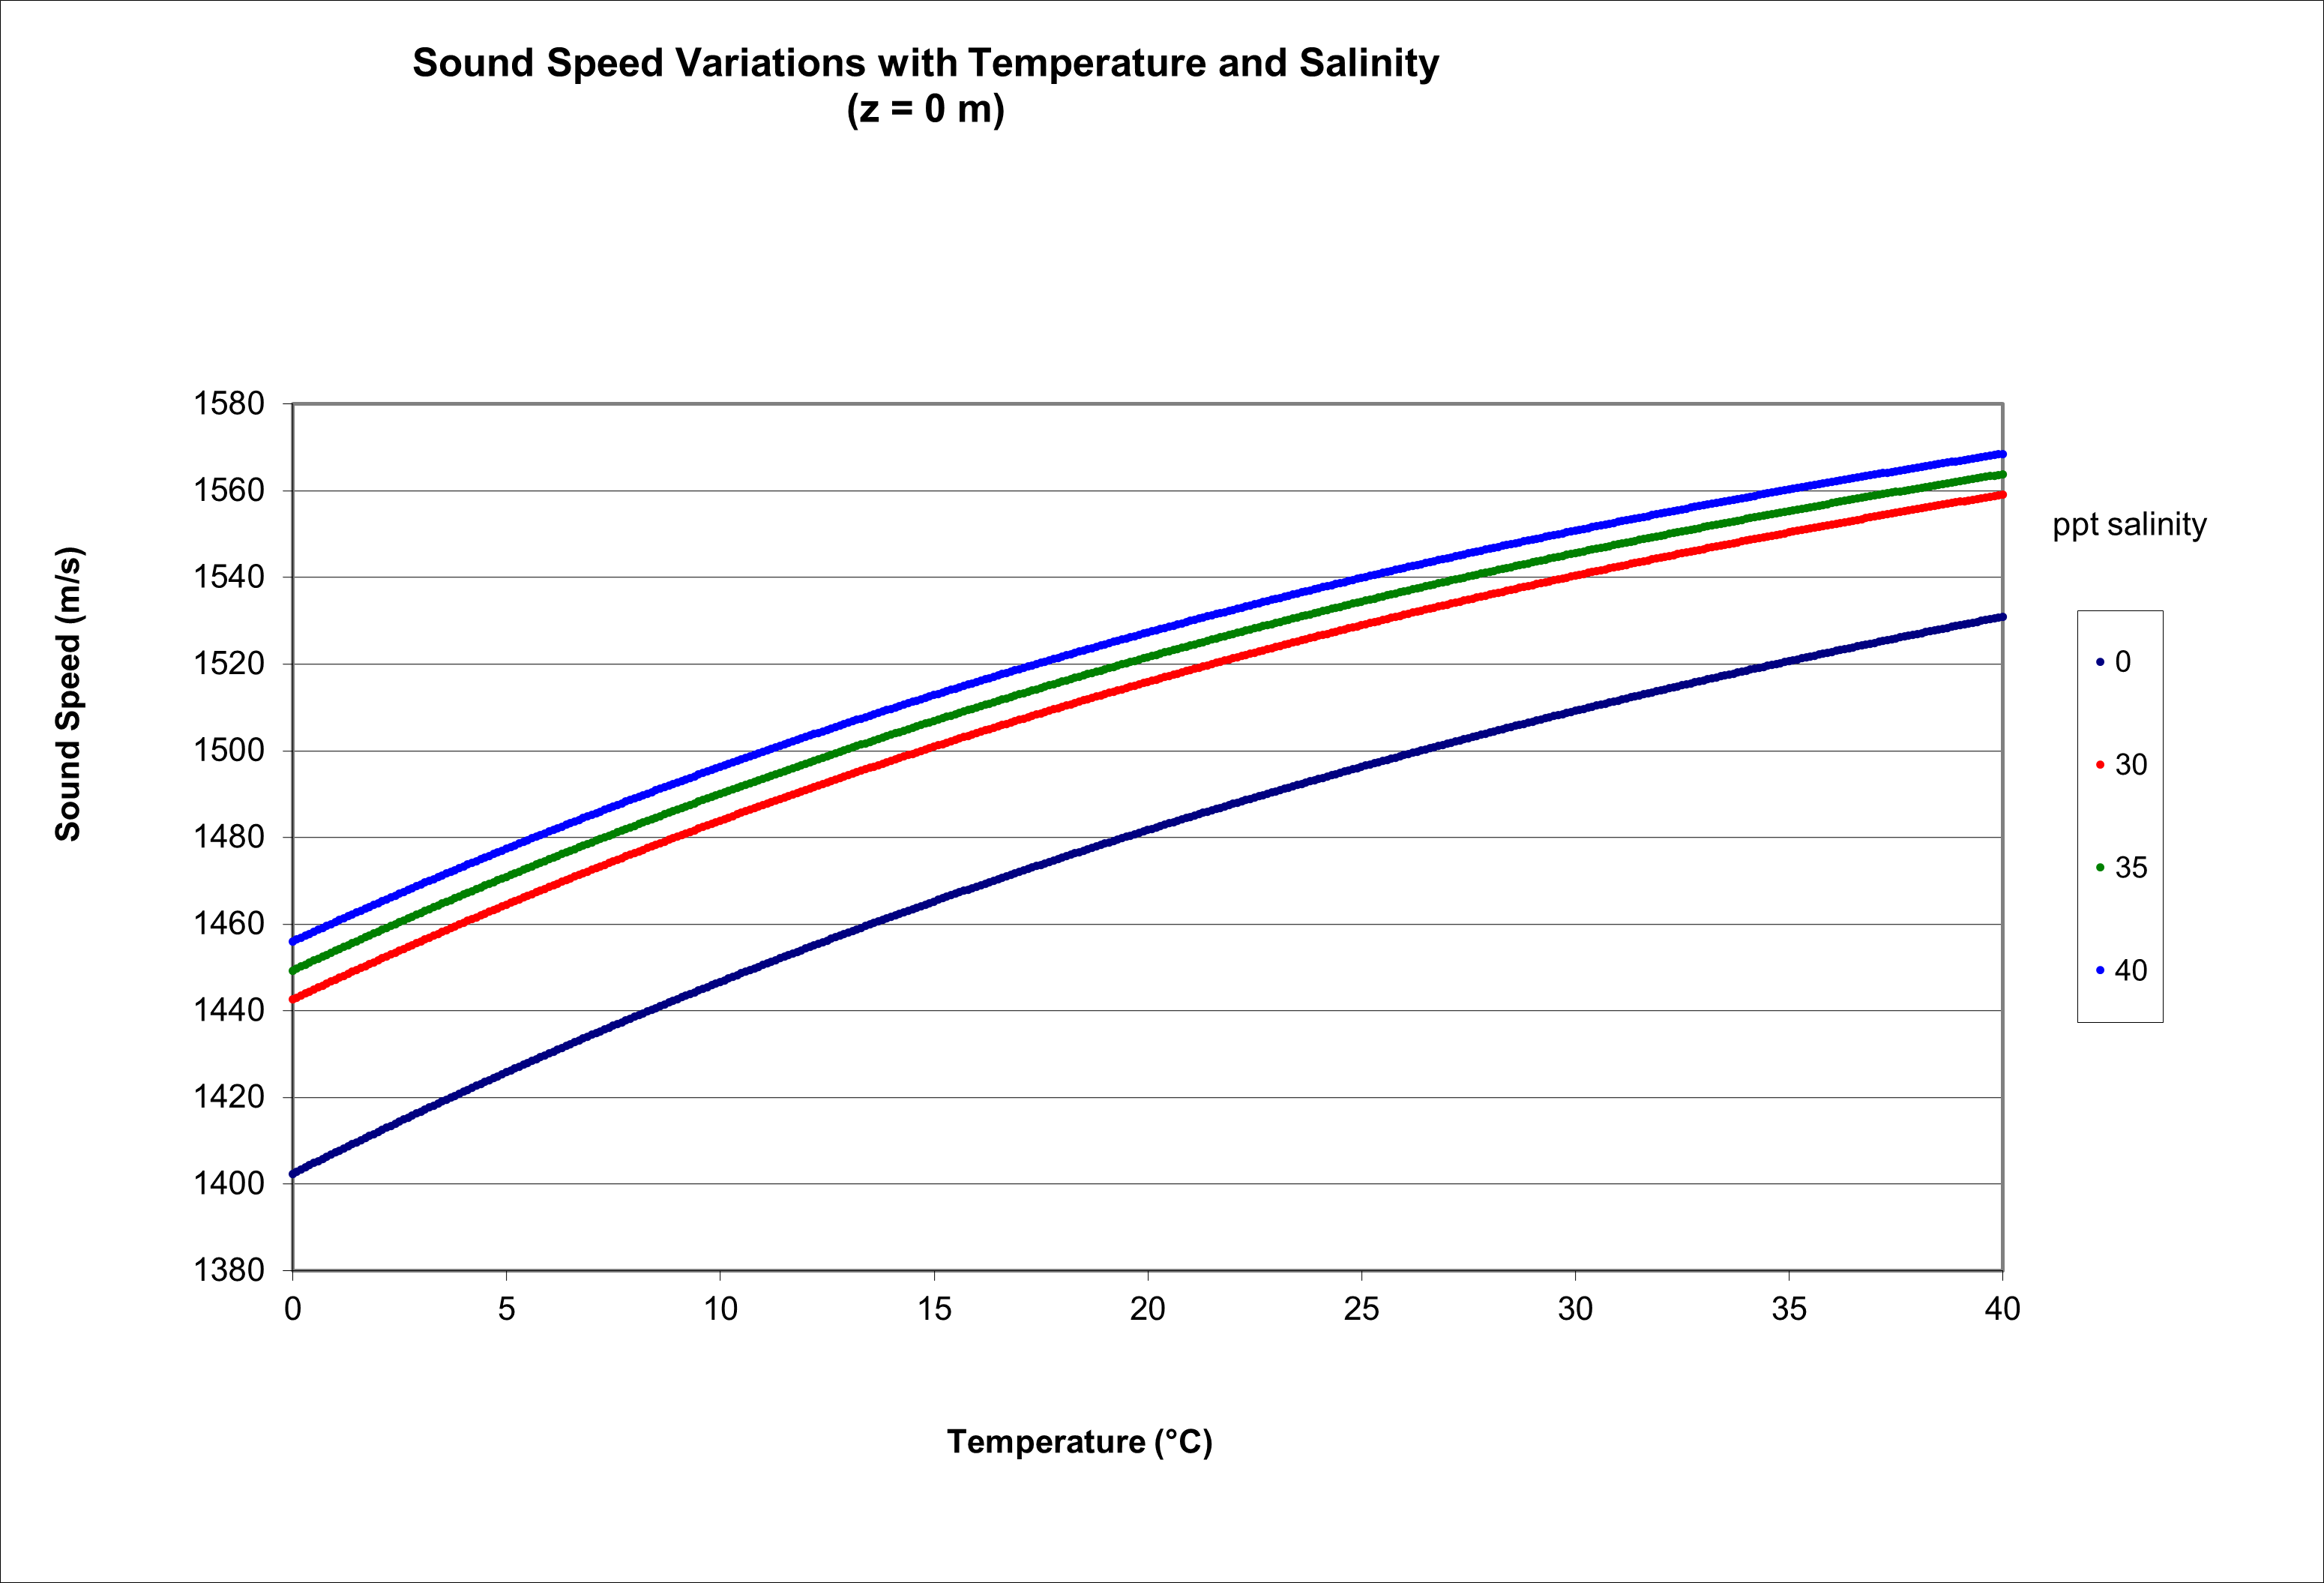
\includegraphics[width=0.8\textwidth]{images/3_15.png}
\end{figure}


\subsection{Spherical Waves}

The wave equation for 3D waves:
   \[
   \nabla^2 p = \frac{1}{c^2} \frac{\partial^2 p}{\partial t^2}.
   \]
   is valid in any reference system, but the form of \(\nabla^2\) changes depending on the chosen coordinate system.

\begin{itemize}

\item Cartesian Coordinates (\(x, y, z\)) are convenient for describing plane waves. \begin{figure}[H]
    \centering
    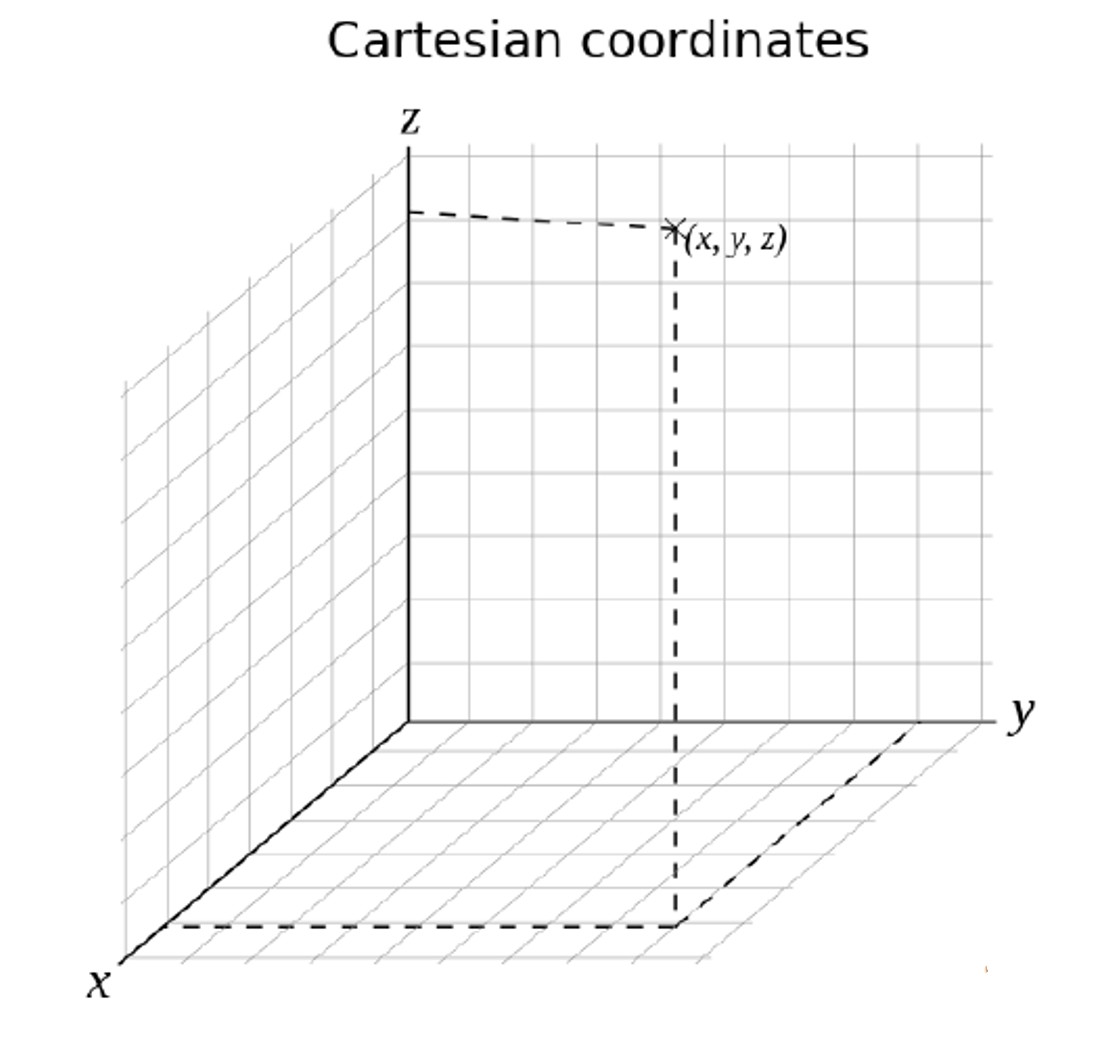
\includegraphics[width=0.5\textwidth]{images/3_17_1.png}
\end{figure} In this system:
     \[
     \nabla^2 = \frac{\partial^2}{\partial x^2} + \frac{\partial^2}{\partial y^2} + \frac{\partial^2}{\partial z^2}.
     \]

\item Cylindrical Coordinates are useful for a line source, where the wavefronts are cylindrical, so the source has a preferred axis.
   Here the coordinates are \(r\) (distance from the axis), \(\phi\) (azimuthal angle), and \(z\) (axis along the source is oriented).
    \begin{figure}[H]
    \centering
    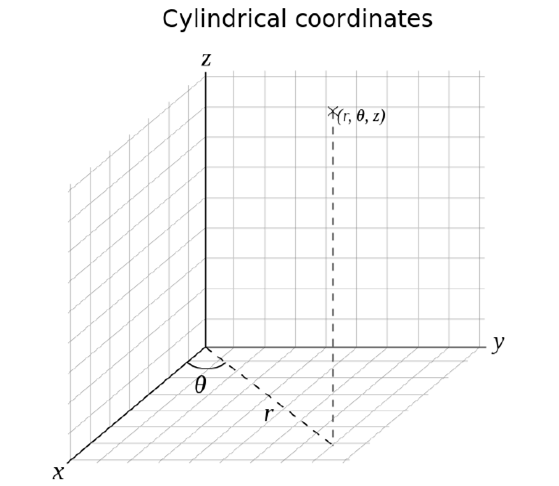
\includegraphics[width=0.5\textwidth]{images/3_17_2.png}
\end{figure}
   The Laplacian operator is:
     \[
     \nabla^2 = \frac{1}{r} \frac{\partial}{\partial r} \left( r \frac{\partial }{\partial r} \right) + \frac{1}{r^2} \frac{\partial^2 p}{\partial \phi^2} + \frac{\partial^2 }{\partial z^2}.
     \]
     
\item Spherical Coordinates are useful for describing waves from a point source, where the wavefronts are spherical.
   Here the coordinates are: \(r\) (distance from the origin), \(\phi\) (azimuthal angle), and \(\theta\) (polar angle). The angular coordinates gives the direction of propagation.
    \begin{figure}[H]
    \centering
    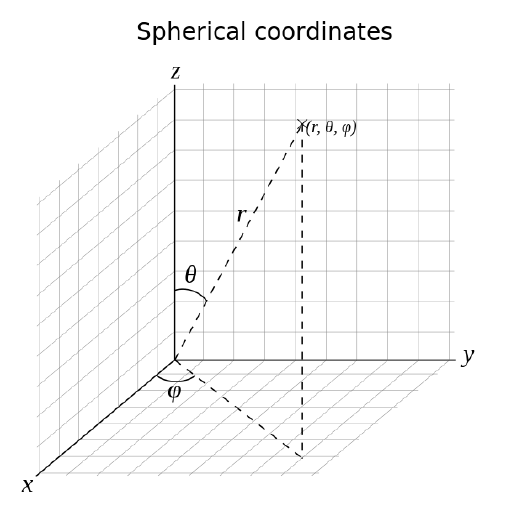
\includegraphics[width=0.5\textwidth]{images/3_17_3.png}
\end{figure}
   The Laplacian operator becomes:
     \[
     \nabla^2 = \frac{1}{r^2} \frac{\partial}{\partial r} \left( r^2 \frac{\partial}{\partial r} \right) + \frac{1}{r^2 \sin \theta} \frac{\partial}{\partial \theta} \left( \sin \theta \frac{\partial}{\partial \theta} \right) + \frac{1}{r^2 \sin^2 \theta} \frac{\partial^2}{\partial \phi^2}.
     \]

     
    
\end{itemize}




In spherical coordinates, the wave equation is given by:
\[ \nabla^2 p = 
\frac{1}{r^2} \frac{\partial}{\partial r} \left[ r^2 \frac{\partial p}{\partial r} \right] + \frac{1}{r^2 \sin \theta} \frac{\partial}{\partial \theta} \left[ \sin \theta \frac{\partial p}{\partial \theta} \right] + \frac{1}{r^2 \sin^2 \theta} \frac{\partial^2 p}{\partial \phi^2} = \frac{1}{c^2} \frac{\partial^2 p}{\partial t^2}.
\]

spherical waves are isotropic, depending solely on the distance from the source, \( r \), so we can neglet angular dependence (\( \partial / \partial \theta = 0 \) and \( \partial / \partial \phi = 0 \)), Applying the product rule to the derivative \( 
\frac{\partial}{\partial r} \left( r^2 \frac{\partial p}{\partial r} \right) = \frac{\partial (r^2)}{\partial r} \frac{\partial p}{\partial r} + r^2 \frac{\partial^2 p}{\partial r^2}
\), the equation reduces to:
\[
\frac{\partial^2 p}{\partial r^2} + \frac{2}{r} \frac{\partial p}{\partial r} = \frac{1}{c^2} \frac{\partial^2 p}{\partial t^2}.
\]

This equation is reminiscent of the plane wave equation but includes an additional term \( \frac{2}{r} \frac{\partial p}{\partial r} \), indicating that plane waves are not solutions to this equation. Instead, the solutions are spherical waves.

To simplify further, we assume that the solution to spherical wave equation is \( p(r, t) = \frac{1}{r} f(r, t) \), substituting this into the equation:
\[
\frac{\partial^2 f}{\partial r^2} = \frac{1}{c^2} \frac{\partial^2 f}{\partial t^2}.
\]

This results in the standard wave equation for \( f(r, t) \), which has the general solution:
\(
f(r, t) = f(r - ct).
\)

Thus, the pressure wave is expressed as:
\[
p(r, t) = \frac{1}{r} f(r - ct).
\]

This solution reveals that the pressure amplitude of a spherical wave decreases proportionally to \( \frac{1}{r} \) as it propagates away from the source.


The intensity of the wave, a measure of the energy it carries, is proportional to the square of the pressure:
\[
I \propto p^2 \propto \frac{1}{r^2}.
\]

This relationship ensures energy conservation. As the wave propagates outward, the surface area of the spherical wavefront increases, distributing the energy over a larger area, leading to a decrease in local intensity. The total energy remains constant, given by the integration of the intensity over the spherical surface.

Instruments typically emit sound as spherical waves, even if the initial radiation pattern is complex. At sufficient distances, the waves can be approximated as emanating from a point source. Locally, these waves can further be approximated as plane waves, especially when observed far from the source. This approximation significantly simplifies wave analysis in practical applications.

Another consideration is the direction of propagation. While mathematically, spherical waves can propagate inward or outward, in practice, we consider only outward-propagating waves, as they correspond to sound emanating from a source.

\section {Energy, intensity, pressure level, and attenuation of sound}

In the analysis of simple oscillatory systems, such as a mass on a spring or wave propagation in strings and fluids, we have primarily focused on the dynamics of displacement, velocity, acceleration, and forces using Newton's laws. However, it is equally important to analyze these systems from the perspective of energy, particularly the principle of energy conservation. This principle provides a powerful tool for understanding the dynamics of oscillatory systems.

\subsection{Simple Oscillator}

For a simple harmonic oscillator, where a mass is attached to a spring, we define two forms of energy: kinetic energy, \(E_K(t)\), and potential energy, \(E_P(t)\). The potential energy depends on the restoring force exerted by the spring. The kinetic energy is determined by the velocity of the mass.

The kinetic and potential energy are given by:
\[
E_K(t) = \frac{1}{2} m v(t)^2, \quad E_P(t) = \frac{1}{2} k x(t)^2,
\]
where \(m\) is the mass, \(v(t)\) is its velocity, \(k\) is the spring constant, and \(x(t)\) is the displacement of the mass from the equilibrium position.



The infinitesimal work done on a mass can be expressed as the infinitesimal change in kinetic energy:

\[
\delta \mathcal{L} = \vec{F} \cdot d\vec{s} = m \, \vec{a} \cdot d\vec{s} = m \, \frac{d\vec{v}}{dt} \cdot d\vec{s} = m \, d\vec{v} \cdot \frac{d\vec{s}}{dt} = m \, d\vec{v} \cdot \vec{v} = d\left(\frac{1}{2} m v^2\right),
\]

where the derivative of the squared velocity is given by:

\[
d(v^2) = d(\vec{v} \cdot \vec{v}) = 2 \, \vec{v} \cdot d\vec{v}.
\]

Thus, the total work done on the mass is determined by measuring its initial and final velocities:

\[
\mathcal{L}_{A \to B} = \frac{1}{2} m v_B^2 - \frac{1}{2} m v_A^2 \quad \forall \, \vec{F}.
\]

If the force is conservative, the work done between two points depends solely on their positions, regardless of the path taken. This property allows the definition of a potential energy function, \(E_P\), such that:

\[
\mathcal{L}_{A \to B} = -\Delta E_p \implies \Delta E_p = -\int_A^B \vec{F} \cdot d\vec{s}.
\]


The change in potential energy, \(\Delta E_p\), can be computed as:

\[
E_p(x) - E_p(0) = -\int_0^x (-kx) \, dx = \frac{1}{2} kx^2.
\]




During oscillatory motion (\ref{fig:1_17}), energy continuously transforms between kinetic and potential forms. At maximum elongation (\(x(t) = \hat{x}\)), the velocity is zero, and the potential energy is maximum:
\[
E_P = \frac{1}{2} k \hat{x}^2, \quad E_K = 0.
\]
At the equilibrium position (\(x(t) = 0\)), the displacement is zero, and the velocity is maximum:
\[
E_K = \frac{1}{2} m \hat{v}^2, \quad E_P = 0.
\]

These relations can be analyzed analytically. For a harmonic oscillator, the displacement and velocity are:
\[
x(t) = \hat{x} \cos(\omega t + \phi), \quad v(t) = -\hat{x} \omega \sin(\omega t + \phi),
\]
where \(\hat{x}\) is the amplitude, \(\omega\) is the angular frequency, and \(\phi\) is the phase. Substituting these expressions into the energy equations, we find:

\[
E_K(t) = \frac{1}{2} k \hat{x}^2 \sin^2(\omega t + \phi), \quad E_P(t) = \frac{1}{2} k \hat{x}^2 \cos^2(\omega t + \phi).
\]

These two energy components have the same amplitude, but \(E_K(t)\) oscillates as the square of a sine function, while \(E_P(t)\) oscillates as the square of a cosine function. Both energies are always positive and oscillate in counterphase: when one reaches its maximum, the other is at its minimum.

\begin{figure}[H]
    \centering
    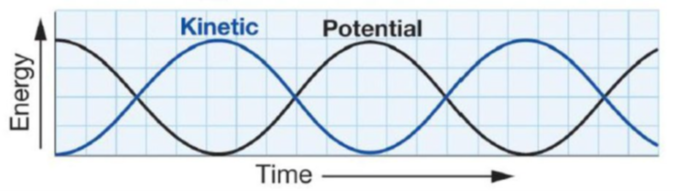
\includegraphics[width=0.7\textwidth]{images/4_2.png}
\end{figure}

The total energy of the system remains constant over time, as only conservative forces are acting. \[E_\text{total} = E_K(t) + E_P(t) = \frac{1}{2} k \hat{x}^2, \quad \Delta (E_K + E_P) = 0
\]

The principle of energy conservation states that the work done on the system, \(\mathcal{L}\), results in changes in its energy:
\[
\mathcal{L} = \Delta E_K = -\Delta E_P 
\]


This principle is valid as long as there are no dissipative forces, such as friction, in the system.\\


\subsection{Damped Oscillator}

A simple oscillator will oscillates indefinitely because there is no dissipation and no external work being done (except for the work of the elastic force). However, if we consider a damped oscillator, friction or other dissipative forces will gradually reduce its motion unless we supply an external force (\ref{fig:1_19}). To sustain periodic motion in such a system, we need to provide an external force, typically a harmonic force.

\[
f(t) = \hat{f} \cos(\Omega t), \quad v(t) = \hat{v} \cos(\Omega t + \Phi').
\]

where \(\hat{f}\) and \(\hat{v}\) represent the amplitudes, \(\Omega\) is the angular frequency, and \(\Phi'\) is the phase difference between them.

The instantaneous power delivered to the oscillator is given by:

\[
P = \frac{\delta \mathcal{L}}{dt} = f \cdot \frac{ds}{dt} = f \cdot v = \frac{1}{2} \hat{f} \hat{v} [\cos(\Phi') + \cos(2\Omega t + \Phi')].
\]

This expression contains two terms:
\begin{itemize}
    \item  The first term, \(\frac{1}{2} \hat{f} \hat{v} \cos(\Phi')\), represents the \textbf{active power or average power}. This is the actual power delivered to the system to sustain its oscillations by compensating for energy losses due to damping.
\item The second term, \(\frac{1}{2} \hat{f} \hat{v} \cos(2\Omega t + \Phi')\), is the \textbf{reactive power}, which oscillates with time around a zero mean. Reactive power represents the energy exchanged back and forth between the oscillator and the external driving force without contributing to net energy transfer over a full cycle.
\end{itemize}

The active power can also be expressed in terms of the impedance \(Z\) of the system:
\[
P_{\text{act}} = \frac{1}{2} \hat{v}^2 \Re[Z] = \frac{1}{4} (f v^* + f^* v) = \frac{1}{2} \Re[f v^*],
\]
where \(f\) and \(v\) are represented in complex notation and \(\frac{1}{2}\hat{v}^2\) represents the root mean square value of the velocity amplitude.

In a damped oscillator with an external driving force, energy must be continuously supplied to counteract the dissipative effects (friction or damping). This energy corresponds to the active power, which ensures the oscillations are maintained. On the other hand, reactive power represents oscillatory energy transfer between the system and the external source, which does not contribute to the sustained motion but oscillates around a mean value of zero.

\subsection{String}

For a string fixed at both ends (\ref{fig:2_20}), the length of the string imposes constraints on the possible wavelengths. Only specific wavelengths, corresponding to the fundamental mode and its harmonics, are allowed. The fundamental mode corresponds to a wavelength of \( \lambda_1 = 2L \), where \( L \) is the length of the string, while the higher harmonics correspond to \( \lambda_n = \frac{2L}{n} \), where \( n \) is the mode index. Consequently, the wave vector \( k_n \) and angular frequency \( \omega_n \) are quantized as:

\[
k_n = \frac{2\pi}{\lambda_n} = \frac{\pi n}{L}, \quad \omega_n = 2\pi f_n = 2\pi \frac{c}{\lambda_n} = \frac{\pi n c}{L}.
\]

These quantized values define the standing wave patterns on the string.\\ The displacement \( y(x,t) \) of the string can be expressed as a Fourier series, representing the sum of all possible modes:

\[
y(x, t) = \sum_{n} \left[A_n \cos(\omega_n t) + B_n \sin(\omega_n t)\right] \sin(k_n x) = \sum_{n} C_n \sin(\omega_n t + \phi_n) \sin(k_n x),
\]

where \( A_n, B_n, C_n, \) and \( \phi_n \) are coefficients that depend on the initial conditions of the string.

The fact that the solution can be expressed as a product of two terms—one depending on time and the other on space—is a characteristic of standing waves. A standing wave arises from the superposition of two counter-propagating traveling waves of the same frequency and amplitude. Because of this symmetry, there is no net propagation of energy in the string, and the wave appears stationary on average.

The velocity \( v(x, t) \) of each individual element of the string at position \( x \) is derived from the displacement \( y(x, t) \):

\[
v(x, t) = \sum_{n} \omega_n C_n \cos(\omega_n t + \phi_n) \sin(k_n x).
\]

Each infinitesimal segment of the string, with mass \( \mu dx \) (\( \mu \) being the linear mass density), oscillates up and down under the restoring force provided by the tension in the string. This behavior is analogous to the oscillations of a spring, where kinetic energy alternates with potential energy. Due to the restoring force, energy accumulates alternately in the form of kinetic energy and potential energy. These two forms of energy oscillate in counterphase: when the kinetic energy is at its maximum, the potential energy is at its minimum, and vice versa. The total energy of the system, however, remains constant, as the maximum value of the kinetic or potential energy represents the total energy stored in the string.

By analyzing the kinetic energy, we can calculate its maximum value, which will allow us to determine the total energy of the string. With the waveform fully defined, the total energy of the system can be expressed and evaluated.



Starting from the velocity of each individual element of the string, \(v(x,t)\), we calculate the infinitesimal kinetic energy for an element of mass \(dm\):
\[
dE_{n} = \frac{1}{2} (dm) v^2(x,t).
\]
Substituting the mass element \(dm = \mu dx\), where \(\mu\) is the linear mass density, and considering the expression for \(v(x,t)\), we can compute the maximum kinetic energy \(dE_{n}^{\text{max}}\) for the string element:
\[
dE_{n}^{\text{max}} = \frac{1}{2} \mu v_{\text{max}}^2(x) dx = \frac{1}{2} \mu \omega_n^2 C_n^2 \sin^2(k_n x) dx.
\]

To find the total maximum kinetic energy for mode \(n\), we integrate over the length of the string:
\[
E_{n}^{\text{max}} = \int_0^L dE_{n}^{\text{max}} = \frac{1}{4} \omega_n^2 \mu L C_n^2,
\]
where \(C_n\) represents the amplitude of the mode \(n\), \(\omega_n\) is the angular frequency, and \(L\) is the length of the string.

Finally, the total maximum energy stored in the string, summing over all modes \(n\), is given by:
\[
E_{\text{TOT}}^{\text{max}} = \sum_{n} E_{n}^{\text{max}}.
\]

Each mode \(n\) contributes to the total energy based on its amplitude \(C_n\) and frequency \(\omega_n\). Importantly, the kinetic energy of each infinitesimal mass depends on its position along the string, as indicated by the \(\sin^2(k_n x)\) term. For certain points along the string (e.g., nodes), the kinetic energy will always be zero.


\subsection{Sound Intensity and Energy Density in Sound Waves}

 Sound wave propagation can be described using two perspectives: the motion and interaction of fluid molecules (via Newton's laws and mass conservation) and the propagation of energy (through energy density and sound intensity).


When a sound wave propagates, it exerts pressure on the fluid molecules, causing them to accelerate. Newton's second law relates this pressure gradient (\(\nabla p\)) to the acceleration of the molecules. For a progressive wave, the relations between pressure and velocity, and the subsequent wave equation, are expressed as:

\[
\begin{cases}
\nabla p = -\rho_0 \frac{\partial \vec{v}}{\partial t} \\
\rho_0 \nabla \cdot \vec{v} = -\frac{1}{c^2} \frac{\partial p}{\partial t}
\end{cases}
\quad \implies \quad 
\nabla^2 p = \frac{1}{c^2} \frac{\partial^2 p}{\partial t^2}.
\]

This describes the dynamic interaction between pressure variations and particle velocity in the fluid.

Sound waves carry energy, which is evident in the motion of the fluid molecules. Initially at rest, the molecules acquire velocity and kinetic energy when the wave arrives, indicating that the wave carries momentum and energy. This energy can be analyzed in two ways:
\begin{itemize}
    \item \textbf{Energy Density (\(w\))}: The amount of energy per unit volume at a specific point changes as the wave passes.
\item \textbf{Sound Intensity (\(I\))}: The energy transported by the wave per unit area per unit time.
\end{itemize}

\begin{figure}[H]
    \centering
    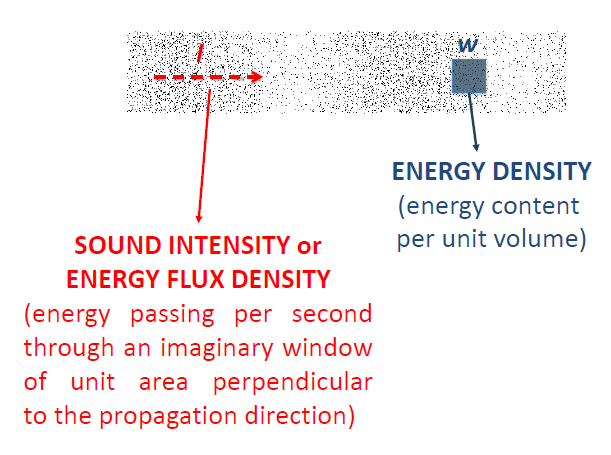
\includegraphics[width=0.5\textwidth]{images/4_6_1.png}
\end{figure}


When a sound wave carries energy into a given region, the energy density in that region changes. The relationship between these quantities is determined by considering a control volume with a surface \(dS\) and length \(c \, dt\), where \(c\) is the wave speed.

\begin{figure}[H]
    \centering
    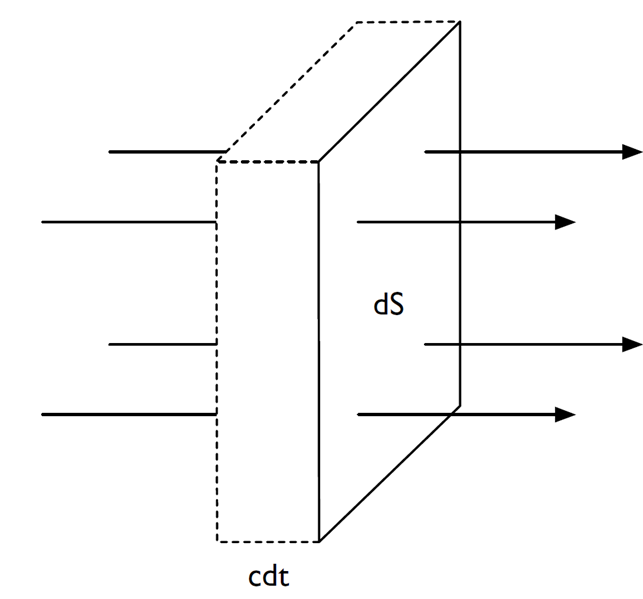
\includegraphics[width=0.4\textwidth]{images/4_6_2.png}
\end{figure}

The energy flow through the surface during the time interval \(dt\) is proportional to the energy stored in the control volume:

\[
I \cdot dt \cdot dS = w \cdot dV = w \cdot c  dt \cdot dS,
\]

which simplifies to:

\[
I = c \cdot w.
\]

This equation demonstrates that the sound intensity \(I\) is proportional to the energy density \(w\), with the wave speed \(c\) as the proportionality factor.


This analysis holds true for a single progressive wave propagating in one direction, as the net transport of energy and momentum is well-defined. However, for counter-propagating waves (e.g., standing waves), there is no net transport of energy or momentum, and the relationship \(I = c \cdot w\) no longer applies. In such cases, energy exists in the system, but there is no measurable intensity due to the absence of a net energy flow.



\subsection{Divergence Theorem}

To analyze the energy balance in the three-dimensional state of a fluid where sound waves propagate, we require a more general description. This description is grounded in two fundamental concepts based on the divergence theorem.

Considering the pressure acting on a surface, let's take into account only the component of the force normal to the surface (not the total force). This component, denoted as \(F_n\), is the projection of the force vector onto the normal to the surface. 
\begin{figure}[H]
    \centering
    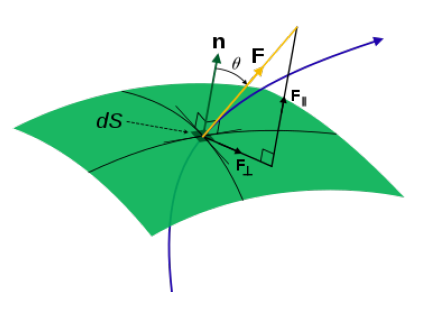
\includegraphics[width=0.4\textwidth]{images/4_7_1.png}
\end{figure}
The \textbf{flux of a vector field \(\vec{F}\) through a generic surface \(A\)} is defined as:

\[
\Phi_F = \iint_A \vec{F} \cdot \vec{n} \, dS.
\]



This formula considers each individual surface element \(dS\), the vector field \(\vec{F}\), and the normal vector \(\vec{n}\) to the surface. The flux describes how much of the vector \(\vec{F}\) passes through the surface \(A\). The meaning of the flux varies depending on the nature of the vector field \(\vec{F}\).

The concept of flux is closely connected to the divergence of a vector field. For example, let's consider a closed surface as a warapped up open surface. For a closed surface, we define the normal vector \(\vec{n}\) for all surface elements.  By convention, the normal vector for a closed surface points outward (all normal vectors must follow the same sign convention).

\begin{figure}[H]
    \centering
    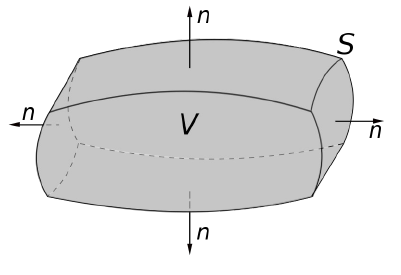
\includegraphics[width=0.4\textwidth]{images/4_7_2.png}
    \caption{Control volume}
    \label{fig:4_7_2}
\end{figure}

The divergence theorem states that the behavior of the vector field \(\vec{F}\) on the surface, in terms of the flux flowing through it, is related to the divergence of the same vector field inside the volume enclosed by the surface. Mathematically, the divergence theorem is expressed as:

\[
\iiint_V (\nabla \cdot \vec{F}) \, dV = \iint_S (\vec{F} \cdot \vec{n}) \, dS.
\]


This theorem indicates that the flux through the surface \(S\) is related to the divergence of \(\vec{F}\) inside the volume \(V\). For instance, if mass flows through the boundary of a volume, the mass density within the volume changes accordingly.

Historically, this theorem has been applied in two main fields: the continuity equation in physics and mathematics, and in solving integrals (as it transforms a surface integral into a volume integral). This relationship is particularly useful in analyzing balance equations where energy, mass, or other quantities enter and exit a control volume.\\




To demonstrate the divergence theorem, we consider a simple geometric shape, such as a rectangular volume \(V\), which serves as a closed volume. This volume has six surfaces, and for the flux calculation, we define normal vectors pointing outward from each surface.

The rectangular volume \(V\) is defined as:
\[
V : \begin{cases}
a \leq x \leq b, \\
c \leq y \leq d, \\
e \leq z \leq f.
\end{cases}
\]

\begin{figure}[H]
    \centering
    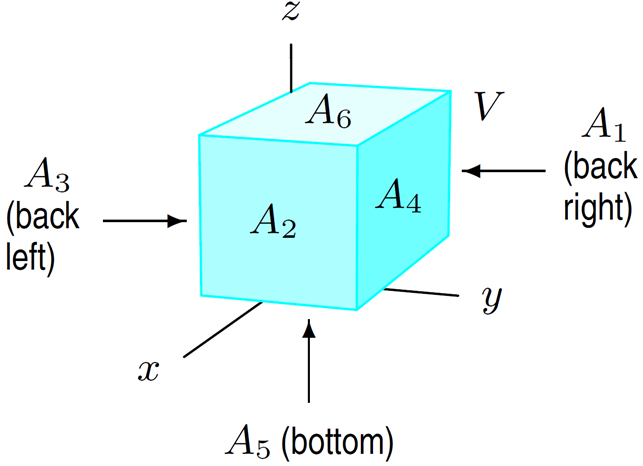
\includegraphics[width=0.4\textwidth]{images/4_8.png}
\end{figure}

We begin by calculating the flux of the vector field \(\vec{F}\) along the \(x\)-direction. The flux through the two surfaces \(A_1\) and \(A_2\), normal to the \(x\)-axis, is given by:
\[
\int_{A_1} \vec{F} \cdot d\vec{A} + \int_{A_2} \vec{F} \cdot d\vec{A} = -\int_e^f \int_c^d F_1(a, y, z) \, dy \, dz + \int_e^f \int_c^d F_1(b, y, z) \, dy \, dz,
\]
which simplifies to:
\[
\int_e^f \int_c^d \left(F_1(b, y, z) - F_1(a, y, z)\right) \, dy \, dz.
\]

Using the fundamental theorem of calculus:
\[
F_1(b, y, z) - F_1(a, y, z) = \int_a^b \frac{\partial F_1}{\partial x} \, dx,
\]
we can write:
\[
\int_{A_1} \vec{F} \cdot d\vec{A} + \int_{A_2} \vec{F} \cdot d\vec{A} = \int_e^f \int_c^d \int_a^b \frac{\partial F_1}{\partial x} \, dx \, dy \, dz = \int_V \frac{\partial F_1}{\partial x} \, dV.
\]



Repeating the process for the \(y\)- and \(z\)-directions, we find:
\[
\int_{A_3} \vec{F} \cdot d\vec{A} + \int_{A_4} \vec{F} \cdot d\vec{A} = \int_V \frac{\partial F_2}{\partial y} \, dV,
\]
\[
\int_{A_5} \vec{F} \cdot d\vec{A} + \int_{A_6} \vec{F} \cdot d\vec{A} = \int_V \frac{\partial F_3}{\partial z} \, dV.
\]

Summing all these contributions, the total flux through the closed surface \(S\) is:
\[
\int_A \vec{F} \cdot d\vec{A} = \int_V \left( \frac{\partial F_1}{\partial x} + \frac{\partial F_2}{\partial y} + \frac{\partial F_3}{\partial z} \right) \, dV = \int_V \nabla \cdot \vec{F} \, dV.
\]

Thus: \[
\nabla \cdot \vec{F} = 
\left( 
\frac{\partial \hat{\mu}_x}{\partial x} + 
\frac{\partial \hat{\mu}_y}{\partial y} + 
\frac{\partial \hat{\mu}_z}{\partial z} 
\right) \cdot 
\left( 
F_1 \hat{\mu}_x + 
F_2 \hat{\mu}_y + 
F_3 \hat{\mu}_z 
\right)
\]

This demonstrates the divergence theorem, which states that the flux of a vector field \(\vec{F}\) through a closed surface is equal to the volume integral of the divergence of \(\vec{F}\) within the enclosed volume:
\[
\int_A \vec{F} \cdot d\vec{A} = \int_V \nabla \cdot \vec{F} \, dV.
\]

\subsection{Continuity Equation}


The infinitesimal amount of the quantity \( q \) crossing a surface element \( S \) in a time interval \( dt \) can be expressed as:
\[
dq = \rho \, dS \, v \, dt,
\]
where \( \rho \) is the density of \( q \), \( v \) is the velocity normal to the surface, and \( dS \) is the surface element. Therefore, the rate of change of \( q \) can be written as:
\[
\frac{dq}{dt} = \rho \, v \, dS = \iint_S \vec{J} \cdot \vec{n} \, dS,
\]
where \(\vec{J} = \rho \vec{v}\) is the flux vector of \( q \). By defining \( \vec{J} \), we automatically account for the portion of the velocity normal to the surface. Thus, the rate of change of the quantity is expressed as the flux of the quantity through the surface. It is important to note that, in physics, the term "flux" generally refers to the surface integral \(\iint_S \vec{J} \cdot \vec{n} \, dS\), rather than to the vector \( \vec{J} \) itself.


The \textbf{integral form} of the continuity equation, including sources or sinks, becomes:
\[
\frac{dq}{dt} + \iint_S \vec{J} \cdot d\vec{S} = \Sigma,
\]
where \( \Sigma \) represents the total contribution of sources and sinks.



Using the divergence theorem (and  \(
     q = \int_V \rho \, dV,
     \)), the integral form can be transformed into the \textbf{differential form}:
\[
\iiint_V \frac{\partial \rho}{\partial t} \, dV + \iiint_V (\nabla \cdot \vec{J}) \, dV = \iiint_V \sigma \, dV
\quad \implies
\frac{\partial \rho}{\partial t} + \nabla \cdot \vec{J} = \sigma.
\]
where \( \sigma \) is the density of sources or sinks, and \( \nabla \cdot \vec{J} \) represents the divergence of \( \vec{J} \). This relationship is valid point by point and provides a localized description of the conservation law. 


The continuity equation establishes a relationship between:
\begin{itemize}
    \item The rate of change of \( q \) within a volume.
    \item The net flux of \( q \) across the boundary of the volume.
    \item The creation or destruction of \( q \) due to sources (\( \sigma > 0 \)) or sinks (\( \sigma < 0 \)).
\end{itemize}



As we said, the direction of the normal vector \(\vec{n}\) is arbitrary. However, for a closed surface, \(\vec{n}\) conventionally points outward. In the integral form without sources and sinks:
\begin{itemize}
    \item  A positive flux (\( \iint_S \vec{J} \cdot \vec{n} \, dS > 0 \)) implies \( q \) is leaving the volume, reducing the total quantity inside.
\item A negative flux (\( \iint_S \vec{J} \cdot \vec{n} \, dS < 0 \)) implies \( q \) is entering the volume, increasing the total quantity inside.
\end{itemize}


\subsection {Sound Waves in Fluids}

We aim to apply the concept of continuity to the energy of sound waves. 

During wave propagation, there are continuous alternating phases of compression and rarefaction, which are associated with changes in pressure. Specifically, regions of the fluid with higher pressure push towards regions of lower pressure. This movement can be visualized through imaginary surfaces within the fluid, where energy is exchanged back and forth.
\begin{figure}[H]
    \centering
    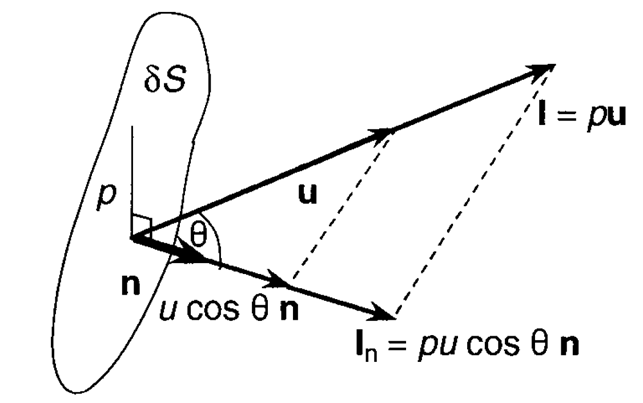
\includegraphics[width=0.5\textwidth]{images/4_11.png}
\end{figure}

The rate of work (power) done by the fluid on one side of an element \( \delta S \) to the fluid on the other side is given by:
\[
P = \frac{dW}{dt} = \vec{F} \cdot \vec{v} = p \, \delta S \, \vec{n} \cdot \vec{v},
\]
where \( \vec{F} \) is the force applied on the surface \( \delta S \), \( p \) is the pressure, \( \vec{n} \) is the normal vector to the surface, and \( \vec{v} \) is the velocity of the particles in the fluid.

The rate of work per unit surface is therefore:
\[
\frac{1}{\delta S} \frac{dW}{dt} = p \, \vec{n} \cdot \vec{v}.
\]


By integrating over a finite surface \( S \), the total power exchanged through the surface can be expressed as:
\[
\iint_S p \, \vec{n} \cdot \vec{v} \, dS = \iint_S \vec{I} \cdot \vec{n} \, dS,
\]
where \( \vec{I} = p \vec{v} \) represents the intensity vector.

The intensity \( \vec{I} \) corresponds to the flux of energy across the surface due to pressure and velocity. Thus, the power exchanged through a surface is directly related to the intensity passing through that surface. This concept underlines how regions of high pressure in a sound wave transfer energy to regions of lower pressure, ultimately describing the energy dynamics of wave propagation.\\



Now we return to the general framework of \(q\), \(\rho\), and \(\vec{J}\). Here, \(q\) represents the total energy in the system, \(\rho\) corresponds to the energy density (\(w\)), and \(\vec{J}\) represents the energy flux, also called intensity (\(\vec{I}\)). An essential observation is that the units of pressure are equivalent to the units of energy density, highlighting the relationship between these quantities in the propagation of sound waves (negletting sources and sinks). Using the principles of continuity and balance equations, we now map these quantities onto the energetic aspects of sound waves.

The \textbf{integral form of the energy continuity equation} relates the rate of change of total energy within a control volume to the net flux of energy through its surface:

\[
\iint_S \vec{I} \cdot \vec{n} \, dS = -\frac{dE}{dt}.
\]

Here:
\begin{itemize}
    \item \(\vec{I} = w \vec{v}\) is the intensity vector.
\item \(E = \iiint_V w \, dV\) represents the total energy stored in the volume, where \(w\) is the energy density.
\end{itemize}

Using the divergence theorem, the \textbf{differential form of the energy continuity equation} can be derived. This equation describes the local energy balance at each point in space:

\[
\nabla \cdot \vec{I} = -\frac{\partial w}{\partial t}.
\]

In this equation:
\begin{itemize}
\item The term \(\nabla \cdot \vec{I}\) is the divergence of \(\vec{I}\).
\item The term \(-\frac{\partial w}{\partial t}\) captures the local rate of change of energy density.
\end{itemize}


 If the intensity vector \(\vec{I}\) is uniform across the space, the divergence \(\nabla \cdot \vec{I}\) becomes zero, indicating no net energy flow or local change in energy density. Conversely, if the intensity varies spatially, there will be a local change in energy density due to energy flow, as indicated by the equation.

These equations establish a connection between two perspectives on energy:
\begin{itemize}
    \item   The local perspective, focusing on the change in energy density (\(w\)).
\item The flux perspective, focusing on the flow of energy (\(\vec{I}\)).
\end{itemize}
These general forms of energy continuity equations will serve as tools to analyze sound waves in a variety of scenarios, allowing for the integration of spatial and temporal energy dynamics.\\





Energy in a sound wave can be classified into kinetic energy and potential energy. The kinetic energy arises from the motion of the molecules when the wave propagates through the medium. On the other hand, to increase the pressure in a region, work must be done on the volume, which leads to the storage of potential energy.

The divergence of the intensity vector \( \nabla \cdot \vec{I} \), which is associated with the rate of change of energy density, can be expressed as the sum of two terms: one involving the time derivative of \( v^2 \), representing the kinetic energy, and the other involving the time derivative of \( p^2 \), representing the potential energy. 

\[
\nabla \cdot \vec{I} = \nabla \cdot (p \vec{v}) = \vec{v} \cdot \nabla p + p \nabla \cdot \vec{v}
\]

Using the differential relations between \( p \) and \( \vec{v} \), derived earlier ( \ref{eq:acoustic_wave_equations_3D}):

\[
\nabla \cdot \vec{I} = -\rho_0 \vec{v} \cdot \frac{\partial \vec{v}}{\partial t} - \frac{1}{\rho_0 c^2} p \frac{\partial p}{\partial t}
\]

This can be rewritten as:

\[
\nabla \cdot \vec{I} = -\rho_0 \frac{\partial}{\partial t} \left( \frac{1}{2} v^2 \right) - \frac{1}{\rho_0 c^2} \frac{\partial}{\partial t} \left( \frac{1}{2} p^2 \right)
=
 -\frac{\rho_0}{2} \frac{\partial v^2}{\partial t} - \frac{1}{2 \rho_0 c^2} \frac{\partial p^2}{\partial t}
\]



So, the rate of change of the total energy density \( w \) is therefore associated with a term proportional to velocity, representing the kinetic energy, and a term proportional to the pressure, representing the potential energy.
\[
 \nabla \cdot \vec{I} = - \frac{\rho_0}{2} \frac{\partial v^2}{\partial t} - \frac{1}{2 \rho_0 c^2} \frac{\partial p^2}{\partial t} = - \frac{\partial w}{\partial t} 
\] \\





The analysis of energy in sound waves can be performed in terms of instantaneous intensity or time-averaged quantities. The intensity is defined as:
\[
\vec{I}(t) = p \vec{v} \quad \text{(Instantaneous intensity)},
\]
\[
\overline{\vec{I}} = \overline{p \vec{v}} \quad \text{(Time-averaged intensity)}.
\]

Using complex notation, the time-averaged intensity can be expressed as:
\[
\overline{\vec{I}} = \frac{1}{4} (p \vec{v}^* + p^* \vec{v}) = \frac{1}{2} \Re[p \vec{v}^*].
\]

From the continuity equation for energy, the divergence of the time-averaged intensity relates to the rate of change of energy density:
\[
\nabla \cdot \overline{(p \vec{v})} = - \frac{\rho_0}{2} \frac{\partial \overline{v^2}}{\partial t} - \frac{1}{2 \rho_0 c^2} \frac{\partial \overline{p^2}}{\partial t} = -\frac{d\overline{w}}{dt}.
\]

The energy density \(\overline{w}\) can be decomposed into two terms:
\[
\overline{w} = \frac{\rho_0}{2} \overline{v^2} + \frac{\overline{p^2}}{2 \rho_0 c^2} = \overline{w}_{\text{kin}} + \overline{w}_{\text{pot}},
\]
where:
\begin{itemize}
    \item \(\overline{w}_{\text{kin}} = \frac{\rho_0}{2} \overline{v^2}\) represents the kinetic energy term.
    \item \(\overline{w}_{\text{pot}} = \frac{\overline{p^2}}{2 \rho_0 c^2}\) represents the potential energy term.
\end{itemize}


Integrating over a time interval yields the total energy density, composed of kinetic and potential components. While the total energy is conserved, the potential energy often includes an arbitrary constant, typically set to zero for simplicity.

\subsection{Intensity of Waves}



We are interested in examining the intensity for different types of sound waves to analyze the energy carried by these waves.\\

In the case of \textbf{plane waves}, the computation of intensity requires determining the velocity \( v \). This is a one-dimensional problem, so \( v \) is treated as a scalar. The pressure \( p(x, t) \) and velocity \( v(x, t) \) are wave-like functions dependent on both spatial (\( x \)) and temporal (\( t \)) variables. As a result, the intensity \( I(x, t) \) is also a function of \( x \) and \( t \), reflecting the three-dimensional nature of wave propagation.

For plane waves, the following relationships hold:

\[
p(x, t) = p^+(x, t) + p^-(x, t) = A e^{j(\omega t - kx + \phi_A)} + B e^{j(\omega t + kx + \phi_B)},
\]

\[
v_x(x, t) = \frac{p^+(x, t)}{\rho_0 c} - \frac{p^-(x, t)}{\rho_0 c} = \frac{p^+(x, t)}{Z_0} - \frac{p^-(x, t)}{Z_0} = \frac{p^+(x, t)}{Z^+} + \frac{p^-(x, t)}{Z^-},
\]

where:
\[
Z^+ = +Z_0 = +\rho_0 c, \quad Z^- = -Z_0 = -\rho_0 c.
\]

We first define the instantaneous intensity:
\[
I(x, t) = p(x, t) v_x(x, t) = \frac{[p^+(x, t)]^2}{\rho_0 c} - \frac{[p^-(x, t)]^2}{\rho_0 c}.
\]

The time-averaged intensity is then given by:
\[
\overline{I} = \frac{\left(\widetilde{p^+}\right)^2}{\rho_0 c} - \frac{\left(\widetilde{p^-}\right)^2}{\rho_0 c}.
\]

These formulas are valid for any configuration of plane waves.\\



For a \textbf{progressive plane wave}, the pressure of the plane wave is described by:
\[
p(x, t) = A \cos(\omega t - kx + \varphi_A) 
\]
where \( A \) is the amplitude, \( \omega \) the angular frequency, \( k \) the wave number, and \( \varphi_A \) the phase.


The instantaneous energy density \( w(x, t) \) consists of two components: the kinetic energy density and the potential energy density. The energy density can be expressed as a function of either pressure or velocity. In this case, we use the relation \( v(x, t) = \frac{p(x, t)}{\rho_0 c}\):
\[
w(x, t) = \frac{\rho_0}{2} v^2(x, t) + \frac{p^2(x, t)}{2 \rho_0 c^2} = \frac{p^2(x, t)}{\rho_0 c^2}.
\]

For a progressive wave, the kinetic and potential energy densities are equal:
\[
w_{\text{kin}}(x, t) = w_{\text{pot}}(x, t) = \frac{1}{2} w(x, t) = \frac{A^2}{2 \rho_0 c^2} \cos^2(\omega t - kx + \varphi_A).
\]

The instantaneous intensity \( I(x, t) \) of the wave is:
\[
I(x, t) = p(x, t) v(x, t) = \frac{A^2}{\rho_0 c} \cos^2(\omega t - kx + \varphi_A) = c w(x, t).
\]

We can observe that the intensity is directly proportional to the energy density in the specific case of progressive wave plane.

The mean intensity, averaged over time, is:
\[
\overline{I} = \frac{1}{2} \frac{A^2}{\rho_0 c} = c \overline{w}.
\]

( \(
\overline{I} = \frac{1}{T} \int_0^T I(x, t) \, dt = \frac{A^2}{\rho_0 c} \cdot \frac{1}{T} \int_0^T \cos^2(\omega t - kx + \varphi_A) \, dt = \frac{A^2}{\rho_0 c} \cdot \frac{1}{2}
\) since \(\cos^2(x)\) is a periodic function with a period of \(2\pi\), its average value over one period is well-known and equal to \(\frac{1}{2}\) ).\\


We consider two counterpropagating plane waves with the same amplitude, one traveling to the left and the other to the right. These two waves interfere to form a \textbf{standing wave}. 

The pressure \( p(x, t) \) of the standing wave is given by:
\[
p(x, t) = A \cos(\omega t - kx + \varphi_A) + A \cos(\omega t + kx + \varphi_B) = 2A \cos(\omega t + \varphi_1) \cos(kx + \varphi_2).
\]

The instantaneous energy density \( w(x, t) \) is:
\[
w(x, t) = \frac{\rho_0}{2} v^2(x, t) + \frac{p^2(x, t)}{2 \rho_0 c^2} = \frac{A^2}{\rho_0 c^2} \left[ 1 + \cos(2\omega t + 2\varphi_1) \cos(2kx + 2\varphi_2) \right].
\]
where \( v(x, t) = \frac{p(x, t)}{\rho_0 c} \) was used along with the trigonometric identity \( (\cos a \cos b)^2 = \frac{1}{4} [\cos(2a) + \cos(2b)]^2 \).
The instantaneous intensity \( I(x, t) \) is given by:
\[
I(x, t) = p(x, t) v_x(x, t) = \frac{[p^+(x, t)]^2}{\rho_0 c} - \frac{[p^-(x, t)]^2}{\rho_0 c} = \frac{A^2}{\rho_0 c} \left[ \cos^2(\omega t - kx + \varphi_A) - \cos^2(\omega t + kx + \varphi_B) \right],
\]
and the mean intensity over time is:
\[
\overline{I} = 0.
\]

In the case of standing waves, we observe significant oscillations of instantaneous energy density over time and space. At certain points (nodes), the energy density oscillations vanish, while at others (antinodes), they reach maximum values. Since the waves are perfectly counterpropagating, the time-averaged intensity is zero due to the cancellation of energy flow in both directions.

However, if the two counterpropagating waves have different amplitudes, they do not form a standing wave. In this case, the time-averaged intensity \( \overline{I} \) would not be zero, as there would still be a net flow of energy in the direction of the wave with the greater amplitude.\\


In the case of \textbf{spherical waves}, the amplitude decays as \( 1/r \). This results in the following pressure equation:
\[
p(r, t) = \frac{A}{r} \cos(\omega t - kr + \varphi_A).
\]

The instantaneous energy density is:
\[
w(r, t) = \frac{p^2(r, t)}{\rho_0 c^2} = \frac{A^2}{\rho_0 c^2 r^2} \cos^2(\omega t - kr + \varphi_A).
\]

The instantaneous intensity is given by:

\[
I(r, t) = \frac{A^2}{\rho_0 c r^2} \cos^2(\omega t - kr + \varphi_A) = c \, w(r, t).
\]

As in the case of progressive plane waves, we observe that the intensity is directly proportional to the energy density. This proportionality holds true for a single progressive wave, such as the spherical wave considered here.
The mean intensity, averaged over time, is:
\[
\overline{I} = \frac{1}{2} \frac{A^2}{\rho_0 c r^2} \propto \frac{1}{r^2}.
\]

This shows that the intensity, which represents the flux of energy per unit time and per unit surface, decreases as \( 1/r^2 \). This relationship has significant implications: if we compute the total power \( P \) flowing through a spherical surface of radius \( r \), it is given by:
\[
P = I \cdot 4 \pi r^2.
\]

If we consider a second spherical surface at a larger radius, \( r_2 > r_1 \), we find:
\[
P_1 = P_2,
\]
because \( I \propto 1/r^2 \). This indicates that the total energy carried by the wave remains conserved as it propagates outward from the source, spreading over larger areas while the intensity diminishes proportionally to \( 1/r^2 \).



\subsection{The Sound Pressure Levele}


The measurement of sound intensity is often expressed as the sound pressure level (\(L\)) in decibels (dB). A standard reference pressure \( P_b = 2 \times 10^{-5} \, \text{Pa} \), which represents the faintest pressure variation perceived as sound, is commonly used. On the other hand, the threshold of pain corresponds to \( P_{\text{max}} = 20 \, \text{Pa} \). This implies a dynamic range of six orders of magnitude that our auditory system can perceive. These values are relative to an ambient base pressure of approximately \( 5 \times 10^5 \, \text{Pa} \). Consequently, a whisper represents a pressure change of approximately \( 0.1 \, \text{parts per billion} \), and yet, it is perceivable by our auditory system.
\begin{figure}[H]
    \centering
    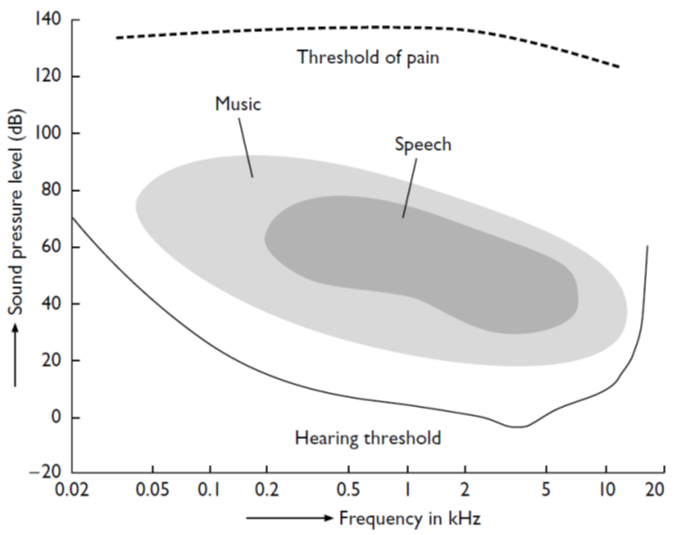
\includegraphics[width=0.6\textwidth]{images/4_19.png}
\end{figure}
To quantify sound levels, a logarithmic scale is employed, reflecting the extensive dynamic range involved. The sound pressure level is calculated using the formula:
\[
L = 20 \cdot \log_{10} \left( \frac{\tilde{p}}{P_b} \right) \, \text{dB},
\]
where \( \tilde{p} \) is the root-mean-square pressure of the sound wave. For comparing two sound pressures, the level difference (\( \Delta L \)) is expressed as:
\[
\Delta L = 20 \cdot \log_{10} \left( \frac{\tilde{p}_1}{\tilde{p}_2} \right) \, \text{dB}.
\]

Due to the logarithmic nature of this scale, the sound pressure level and intensity are proportional to the square of the pressure. This convention ensures that even subtle variations in pressure, spanning over multiple orders of magnitude, are effectively captured and represented.

\subsection{The Attenuation of Sound in Fluids}


Sources of sound include loudspeakers, musical instruments, and other vibrating objects. These sources produce sound waves that propagate through the medium. However, as sound waves travel through a material, part of their energy may be absorbed. This phenomenon is modeled through a thin absorbing material layer. We aim to understand how the intensity (\(I\)) of sound changes as it propagates through an absorbing medium.

The process can be described by considering a thin slab of thickness \(dx\), where the intensity before the slab is \(I\) and after the slab is reduced by an infinitesimal amount \(dI\). 
\begin{figure}[H]
    \centering
    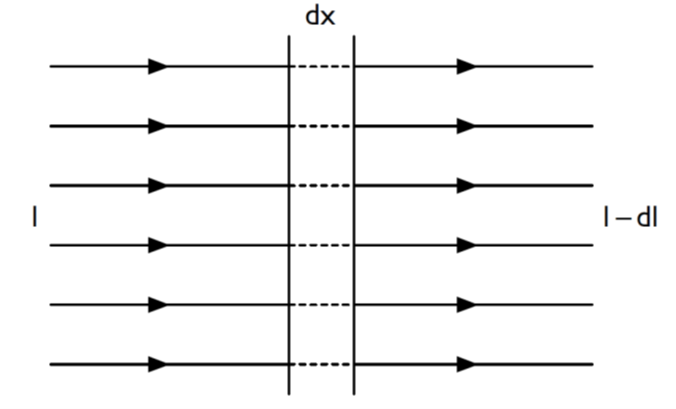
\includegraphics[width=0.5\textwidth]{images/4_20_1.png}
\end{figure}

The amount of energy absorbed is proportional to both the intensity of the wave and the thickness of the slab:
\[
(I - dI) - I = -dI = mI \, dx,
\]
where \(m\) is the absorption coefficient of the material. Solving this differential equation \[ -dI = mI \, dx \quad \to \quad - \frac{dI}{I} = m \,dx \quad \to \quad - \ln\frac{I}{I_0} = m \,x \quad \to \quad  I_0 e^{-mx}   \]  gives the exponential decay of intensity:
\[
I(x) = I_0 e^{-mx},
\]
where \(I_0\) is the initial intensity at \(x = 0\). Since the pressure \(p(x, t)\) is proportional to the square root of intensity, the pressure also decays exponentially:
\[
p(x, t) = p_0 e^{-mx/2} e^{j(\omega t - kx)}.
\]

Linear absorption phenomena result in an exponential decay of intensity as the wave propagates through the medium. The pressure, being proportional to the square root of intensity, also decays exponentially. This explains how sound waves gradually diminish in absorbing materials. If the material efficiently absorbs sound at the interface, the intensity decays exponentially within the material until it dies out. In contrast, when reflection dominates, less energy penetrates the material.

Higher-order, non-linear absorption processes also exist, where the fraction of absorbed intensity depends on the magnitude of the intensity. These processes become relevant at very high intensity levels.

The main reasons for attenuation in gases include:

\begin{itemize}
    \item  \textbf{Non-adiabaticity}: In an ideal isotropic medium, heat exchange between neighboring volumes is negligible. However, in real gases, heat exchange occurs, leading to energy dissipation.
\item \textbf{Friction}: Molecules dissipate energy due to collisions and interactions, similar to how internal stresses in solids dissipate energy.
\item \textbf{Molecular motion}: Molecules possess various degrees of freedom, such as rotational, vibrational, and translational. When energy is transferred to the medium, it can be absorbed by these degrees of freedom, particularly those unrelated to translational motion, reducing the wave's intensity.
\begin{figure}[H]
    \centering
    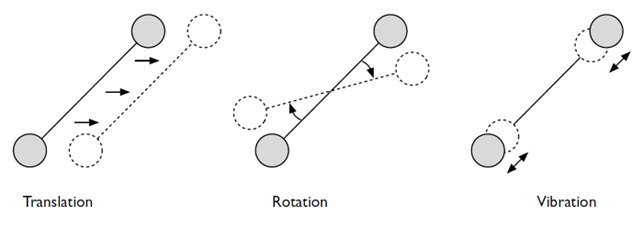
\includegraphics[width=0.6\textwidth]{images/4_20_2.png}
\end{figure}
\end{itemize}




\section{Sound sources and sound radiation}

In this section we explore the physics of sound radiation, starting with a point source and analyzing how this can be modeled mathematically. We aim to describe how multiple point sources can interact, resulting in interference patterns and directional sound radiation. In subsequent sections, we will extend this analysis to continuous vibrating sources and investigate how such systems generate propagating sound waves. This transition from mechanical oscillation to wave propagation will highlight how the characteristics of sound emission depend on parameters such as the size of the source and the wavelength.

\subsection{Spherical Waves}

Spherical waves are prototypical sound waves, propagating uniformly in all directions from a single point source. To analyze these waves, we begin with the three-dimensional wave equation. Applying the Laplace operator in spherical coordinates and assuming isotropic sound propagation (no angular dependence), the wave equation simplifies to:

\[
\frac{\partial^2 p}{\partial r^2} + \frac{2}{r} \frac{\partial p}{\partial r} = \frac{1}{c^2} \frac{\partial^2 p}{\partial t^2}.
\]

By expressing the pressure as \( p(r, t) = \frac{1}{r} f(r, t) \), we observe that the function \( f(r, t) \) satisfies the standard wave equation:

\[
\frac{\partial^2 f}{\partial r^2} = \frac{1}{c^2} \frac{\partial^2 f}{\partial t^2}.
\]

Thus, the solution for the pressure in spherical waves is given by:
\[
p(r, t) = \frac{1}{r} f(r - ct),
\]
where \( c \) is the speed of sound, and \( f(r - ct) \) represents the wave propagating outward.



This solution indicates that the pressure amplitude decays as \( 1/r \), which is consistent with energy conservation. Since the pressure amplitude decreases, the energy flux (intensity) over a spherical surface of radius \( r \) must also decrease to maintain constant total energy.

The instantaneous intensity \( I(r, t) \) of a spherical wave is given by:
\[
I(r, t) = \frac{A^2}{\rho_0 c r^2} \cos^2(\omega t - kr).
\]

The mean intensity, averaged over time, is:
\[
\overline{I} = \frac{1}{2} \frac{A^2}{\rho_0 c r^2} \propto \frac{1}{r^2}.
\]

This relationship highlights the \( 1/r^2 \) decay of intensity, which is a fundamental result of the conservation of energy. As sound propagates outward from a point source, the energy is distributed over an increasing spherical surface area. Consequently, the total power emitted by the source remains constant, while the intensity decreases with the square of the distance.



In summary, the \( 1/r \) decay of pressure and the \( 1/r^2 \) decay of intensity are direct consequences of energy conservation and the spherical geometry of wave propagation. \\


\subsection{Wave Radial Velocity}


We have studied mechanical vibrations and wave propagation separately, but now we aim to establish a connection between them. To do so, we must first address some considerations regarding spherical waves. In our discussions, we often focus on pressure waves, but it is important to recognize that pressure waves are accompanied by velocity waves, which represent oscillating velocity fields in time and space.

To transition from pressure to velocity, we can apply mathematical formalism. Starting from the spherical pressure wave \(
p(r, t) = \frac{A}{r} e^{j(\omega t - kr)},
\), we investigate the velocity vector.

Since sound waves propagate away from the source longitudinally, the velocity vector is radial as well. 
\[
\vec{v} = v_r \vec{u}_r
\]
The force balance equation \(
\vec{\nabla} p = -\rho_0 \frac{\partial \vec{v}}{\partial t}.
\) allows us to calculate the radial velocity derivative:

\[
\frac{\partial v_r}{\partial t} = -\frac{1}{\rho_0} \frac{\partial p}{\partial r}.
\]

Calculated taking in account the nabla operator in spherical coordinates \( 
\vec{\nabla} = \frac{\partial}{\partial r} \vec{u}_r + \frac{1}{r} \frac{\partial}{\partial \theta} \vec{u}_\theta + \frac{1}{r \sin \theta} \frac{\partial}{\partial \phi} \vec{u}_\phi
\) and assuming isotropic radiation, so that we neglect angular dependencies (\(\theta\) and \(\phi\)) in the derivatives, leaving only the radial derivative of the pressure. 


Taking the derivative of the pressure wave with respect to \(r\), which involves a product of functions dependent on \(r\), we find:

\[
\frac{\partial v_r}{\partial t} = \frac{A}{\rho_0 r^2} e^{j(\omega t - kr)} + \frac{A j k}{\rho_0 r} e^{j(\omega t - kr)}.
\]

Integrating over time gives the velocity field:

\[
v_r = \frac{1}{j \omega} \frac{A}{\rho_0} e^{j(\omega t - kr)} \left(\frac{1}{r^2} + \frac{j k}{r}\right) = \frac{p}{\rho_0 c} \left( 1 + \frac{1}{j k r} \right)
\]

This expression shows that the term in brackets, which depends on \(r\), is a complex number. Consequently, the phase of the velocity wave differs from that of the pressure wave. The additional phase, determined by the complex term, depends on the distance \(r\). This implies that spherical waves exhibit a phase shift between the pressure wave oscillation and the velocity wave oscillation, with the phase shift varying with distance.

The behavior of the wave changes significantly depending on the distance from the source:

\begin{itemize}
    \item For \(kr \ll 1\) (short distances, "near field"):
    \[
    v_r \approx \frac{p}{\rho_0 c} \frac{1}{jkr},
    \]
    where the imaginary part dominates, resulting in a 90-degree phase shift between pressure and velocity. As the distance increases, the phase shift transitions from \(90^\circ\) to \(0^\circ\).

    \item For \(kr \gg 1\) (long distances, "far field"):
    \[
    v_r \approx \frac{p}{\rho_0 c},
    \]
    where the real part dominates, and pressure and velocity oscillate in phase.
\end{itemize}



This dual behavior defines two regimes for sound sources:
\begin{itemize}
    \item \textbf{Near field:} The behavior differs significantly, with phase shifts indicating a more complex interaction between pressure and velocity.
    \item \textbf{Far field:} The wavefront behaves like a plane wave because the local radius of curvature becomes large, appearing flat, and the correlation between pressure and velocity matches that of a plane wave.

\end{itemize}



\subsection{Monopole and Volume Velocity}

The prototypical source of a sound wave is the monopole, which can be conceptualized as a very small sphere modulating its own volume over time. This periodic compression and expansion of the sphere create pressure waves that propagate into the surrounding fluid. In this approximation, the monopole behaves as a point source with an infinitesimal radius.
\begin{figure}[H]
    \centering
    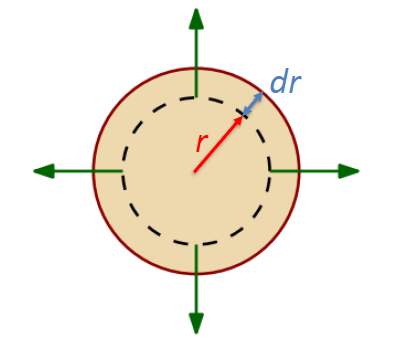
\includegraphics[width=0.4\textwidth]{images/5_4.png}
\end{figure}
The characteristic quantity describing the source's behavior is the \textbf{volume velocity}, \(Q(t)\), defined as the rate of change of the sphere's volume over time. 

To relate the source's properties to the emitted wave, we focus on expressing the wave's amplitude, \(A\), in terms of the source's volume velocity, \(Q(t)\). Let us consider an infinitesimal change in the sphere's volume, \(dV\), due to a change in radius:

\[
dV = \frac{4}{3} \pi (r + dr)^3 - \frac{4}{3} \pi r^3 \approx 4 \pi r^2 dr.
\]



Since \( dr \) is an infinitesimal increment, the terms containing \( (dr)^2 \) and \( (dr)^3 \) are negligible compared to \( dr \). The volume velocity is defined as:
\[
Q(t) = \frac{dV}{dt} = 4 \pi r^2 \frac{dr}{dt} = 4 \pi r^2 v_r,
\]
where \(v_r\) is the radial velocity. Substituting the expression for
\( 
v_r = \frac{p}{\rho_0 c} \left( 1 + \frac{1}{j k r} \right)
\) and \(p(r, t) = \frac{A}{r} e^{j(\omega t - kr)}\),
we obtain:
\[
Q(t) = 4 \pi r^2 \frac{(\frac{A}{r} e^{j(\omega t - kr)})}{\rho_0 c} \left( 1 + \frac{1}{j k r} \right).
\]

In the near-field approximation (\(kr \ll 1\)), so for \(r \to 0\), the term \(1 / (j k r)\) dominates, simplifying the relation:
\[
Q(t) = \frac{4 \pi A}{\rho_0 \omega \, j} e^{j \omega t}
\]


This demonstrates the relationship between the pressure wave's amplitude and the source's volume velocity. The volume velocity determines the radial velocity of the surrounding fluid, which is directly related to the emitted pressure wave. Hence, the amplitude \(A\) of the pressure wave can be fully expressed in terms of the volume velocity \(Q\) of the monopole source. We've also seen that for a point source, \(Q(t)\) oscillates harmonically:

\[
Q(t)= \hat{Q} e^{j \omega t}
\]

The pressure wave emitted by the monopole source can now be expressed as:
\[
p(r, t) = \frac{\rho_0 j \omega \hat{Q}}{4 \pi r} e^{j (\omega t - k r)}.
\]


The mean intensity of the wave, \(\overline{I}\), is proportional to the square of the amplitude:
\[
\overline{I} = \frac{1}{2} \frac{A^2}{\rho_0 c r^2} = \frac{\rho_0 \omega^2 \hat{Q}^2}{32 \pi^2 c r^2}.
\]


\subsection {Directional Factor, Gain, FWHM}

When multiple point sources (monopole) \( Q_1, Q_2, \ldots, Q_N \) with their own volume velocities are distributed over space, the sound perceived by a listener at a position \( P \) results from the interference of these sources.
\begin{figure}[H]
    \centering
    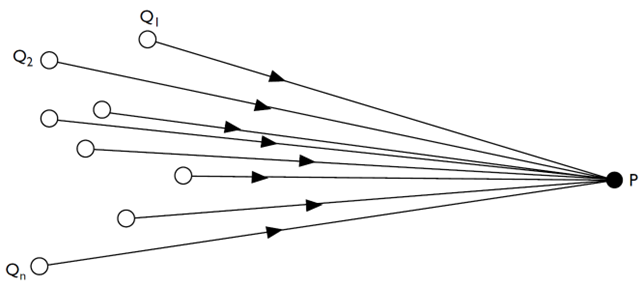
\includegraphics[width=0.6\textwidth]{images/5_5.png}
\end{figure}
Each source may oscillate with a different initial phase, leading to varying accumulated phases (\( kr \)) as the waves propagate different distances to reach \( P \). These differences in phase cause either constructive or destructive interference, depending on the relative phase alignment of the waves.

When two pressure waves of the same amplitude reach a point in phase, their pressures sum, resulting in an intensity four times greater than that of a single wave (\textit{constructive interference}). Conversely, if they are out of phase, they cancel each other out (\textit{destructive interference}), resulting in zero intensity. Importantly, interference redistributes energy spatially without creating or destroying energy. 







To quantify the effect of combining multiple sources, we introduce the \textbf{directional factor}. This is best analyzed in the far field, where each source emits spherical waves, and the wavefront appears spherical from a distance. In this region, the detailed structure of the sources becomes negligible, and interference effects depend only on the relative distances and phases of the sources.

The pressure field in the far field of \( n \) sources is expressed as:
\[
p(r, \theta, \phi, t) = \frac{A}{r} R(\theta, \phi) e^{j(\omega t - kr)},
\]
where \( R(\theta, \phi) \) accounts for the angular variation of intensity due to interference and is usually normalized to 1.

Interference modifies intensity patterns: constructive interference concentrates energy in specific angular directions (main lobes), while destructive interference reduces it in others (side lobes or nulls). This redistribution of energy does not violate conservation laws, as the total radiated energy remains constant.

The radiated intensity is given by:
\[
I(r, \theta, \phi) = \frac{\tilde{p}^2}{Z_0} = \frac{A^2}{2 Z_0 r^2} |R(\theta, \phi)|^2,
\]
where \( \tilde{p} \) is the RMS pressure amplitude and \( Z_0 \) is the acoustic impedance.

where:
\begin{itemize}
    \item \( \tilde{p} \) is the RMS value of the pressure amplitude,
    \item \( Z_0 \) is the acoustic impedance.
\end{itemize}



The term \textit{spherical wave} refers to the wavefront geometry, where points of equal phase expand spherically. However, this does not imply uniform intensity distribution across the wavefront. Some references define \textit{spherical waves} strictly as those with isotropic intensity distributions (no directional factor). For waves with angular-dependent intensity, we describe them as \textit{spherical waves with directional dependence}.


The directional factor \( R(\theta, \phi) \) provides a quantitative characterization of the source's directionality. Engineers often design sources to focus energy in specific angular regions, creating a dominant main lobe. The narrowness of this lobe indicates how much total energy is concentrated within a small angular range.\\





The \textbf{gain} is a measure used to quantify how much of the total intensity is concentrated along the direction of maximum radiation. It is particularly relevant for systems like antenna arrays. The gain is defined as:
\[
\gamma = \frac{I_{\text{max}}}{\langle I \rangle} = 4\pi r^2 \frac{I_{\text{max}}}{P_r},
\]
where \( I_{\text{max}} \) is the maximum intensity, and \( \langle I \rangle \) is the average intensity that would result from an isotropic source emitting the same total power.

The radiated power \( P_r \) is given by:
\[
P_r = \iint_S I(\theta, \phi) \, \text{d}S = \frac{A^2}{2Z_0} \iint_{4\pi} |R(\theta, \phi)|^2 \, \text{d}\Omega.
\]

From this, the gain can be rewritten as:
\[
\gamma = \frac{4\pi}{\iint |R(\theta, \phi)|^2 \, \text{d}\Omega}.
\]



The \textbf{Full Width at Half Maximum (FWHM)} measures the angular width of the main lobe. While it does not quantify the total energy within the lobe, it provides information on how narrow the angular emission is along the main direction of radiation.
\begin{figure}[H]
    \centering
    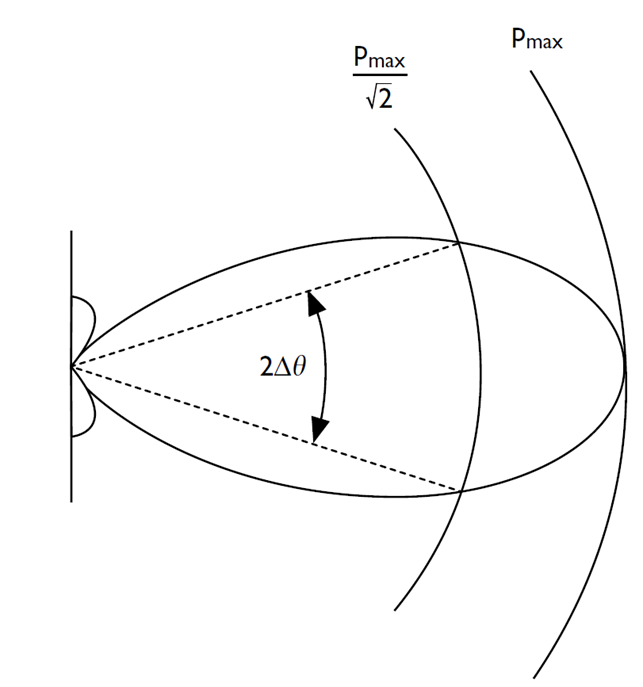
\includegraphics[width=0.4\textwidth]{images/5_6.png}
\end{figure}




In essence, the gain compares the directional source to an ideal isotropic source to determine how much energy is concentrated in the main lobe, while the directional factor provides a more comprehensive picture of intensity distribution.
The directional factor, \( R(\theta, \phi) \), is the most informative quantity for understanding the angular distribution of intensity. The gain, while still useful, provides less detail and is a more general measure. Both of these quantities can be measured experimentally to characterize the directivity of a source.


\subsection{Dipole}

A dipole consists of two monopoles separated by a distance \( d \) and oscillating with opposite phases (180° phase shift). This harmonic oscillation can be expressed as:
\[
Q_{1,2}(t) = \pm \hat{Q} e^{j\omega t}.
\]

If a monopole is conceptualized as a small volume that cyclically expands and contracts, the dipole can be thought of as a system where one monopole fills while the other empties. This oscillatory back-and-forth motion forms the basis of the dipole’s radiation pattern.
\begin{figure}[H]
    \centering
    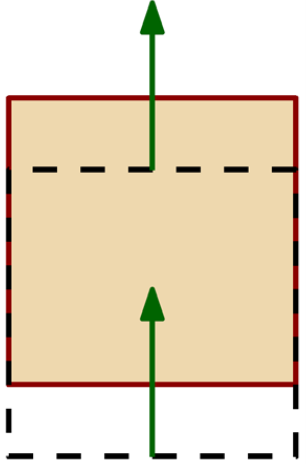
\includegraphics[width=0.1\textwidth]{images/5_7_2.png}
\end{figure}

To analyze the radiation pattern, we examine a generic point \( P \) in the far field, where the distance \( r \) from the sources is much greater than \( d \), the distance between the two monopole. At this distance, the wavefronts reaching \( P \) are approximately spherical. The spherical wave is modulated by a directionality function dependent on the angle \( \theta \) relative to the dipole axis. Since the system is symmetric about the dipole axis, the radiation pattern depends only on \( \theta \), not \( \phi \).

\begin{figure}[H]
    \centering
    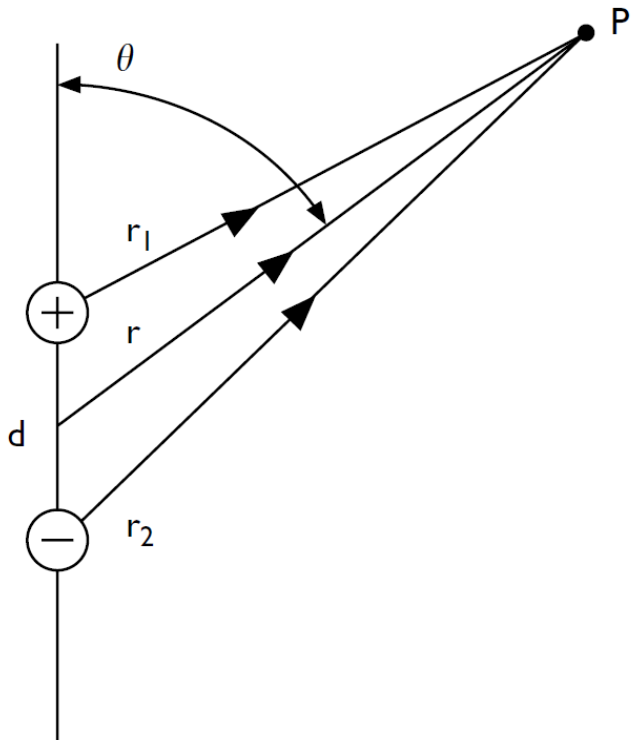
\includegraphics[width=0.4\textwidth]{images/5_7_1.png}
\end{figure}

In the far-field approximation, the distances \( r_1 \) and \( r_2 \) (from each monopole to \( P \)) are nearly parallel. The interference is governed by the initial phase difference of the sources (180° out of phase) and the geometric path difference:
\[
r_{1,2} \approx r \mp \frac{d}{2} \cos\theta,
\]


The phase term in the spherical wave equation depends on \( k r \), where \( k = \frac{2\pi}{\lambda} \) is the wavenumber. Substituting \( r_{1,2} \) into the phase term, the difference in phase between the waves from the two sources becomes:
\[
\Delta \phi = k (r_2 - r_1) = k \left( r + \frac{d}{2} \cos\theta \right) - k \left( r - \frac{d}{2} \cos\theta \right) = k d \cos\theta = \frac{2\pi d}{\lambda} \cos\theta.
\]

This angular dependence of the phase leads to variations in the radiated intensity, which depends on both \( \theta \) and the wavelength \( \lambda \). For a given path difference, the accumulated phase varies, producing an angular radiation pattern that is frequency-dependent.



Considering the contributions from the two sources with a 180° phase shift, the pressure field at P is expressed as:
\[
p(r, t) = \frac{j \omega \rho_0 \hat{Q}}{4 \pi} 
\left(
\frac{e^{-j k r_1}}{r_1} - \frac{e^{-j k r_2}}{r_2}
\right)
e^{j \omega t}.
\]

In the far-field approximation (\( r_1, r_2 \gg d \)), the denominators \( r_1 \) and \( r_2 \) are approximated as \( r \). However, in the exponential terms, the path difference remains significant because the phase depends on the term \( k r \), where \( k = \frac{2\pi}{\lambda} \) is the wavenumber. This means that \( k r \) is directly proportional to \( r/\lambda \), not only \( r \) itself. Even a small difference in the path length can correspond to a considerable fraction of the wavelength, thereby leading to significant phase differences between the two waves. For this reason, while the amplitude terms in the denominator can approximate \( r_1 \) and \( r_2 \) as \( r \) due to their negligible impact, the phase terms in the exponentials must retain the exact path differences to accurately describe the interference. This leads to:
\[
p(r, t) = \frac{j \omega \rho_0 \hat{Q}}{4 \pi r} 
\left(
e^{j\left(\frac{k d}{2} \cos\theta\right)} - e^{-j\left(\frac{k d}{2} \cos\theta\right)}
\right)
e^{j(\omega t - k r)} = - \frac{\omega \rho_0 \hat{Q}}{2 \pi r} 
\sin\left(\frac{k d}{2} \cos\theta\right) 
e^{j (\omega t - k r)}.
\]



The resulting expression shows that the dipole radiation pattern is governed by an angular modulation (
\(
\sin\left(\frac{k d}{2} \cos\theta\right)
\) )
which acts as an envelope over the standard plane wave (\(
\frac{\rho_0 j \omega \hat{Q}}{4 \pi r} e^{j (\omega t - k r)}
\)). This modulation describes the intensity variation as a function of \( \theta \), providing the radiation pattern of a dipole in the far field.\\




Typically, the size of a radiating element is much smaller than the wavelength of the emitted sound. This means that the dipole is not only far away from the observer but is also small relative to the relevant physical quantity of the problem, namely the wavelength. In this situation, we refer to the system as a point dipole. 
\[
kd \ll 1 \quad \to \quad 2\pi \frac{d}{\lambda} \ll 1 \quad \to \quad d \ll {\lambda}
\]

When the distance between the two monopoles is significantly smaller than the wavelength, we can apply further approximations. For very high frequencies, the dipole may no longer behave as a point dipole because of the short wavelength. Conversely, for low frequencies, the approximation of a point dipole remains valid.


The radiation pattern of the dipole depends on the angular position \( \theta \). For a small argument, the sine function can be approximated as:
\[
\sin\left(\frac{k d}{2} \cos\theta\right) \approx \frac{k d}{2} \cos\theta.
\]

Substituting this approximation into the expression for the pressure field in the far field yields:
\[
p(r, t) = -\frac{\omega^2 \rho_0 \hat{Q} d}{4\pi r c} \cos\theta \cdot e^{j(\omega t - k r)}.
\]

This clearly shows that the angular dependence of the radiated intensity is governed by \( \cos\theta \). The radiation is maximum along the axis of the dipole (\( \theta = 0 \)) and minimum in the plane perpendicular to the dipole (\( \theta = \pi/2 \)).

\begin{figure}[H]
    \centering
    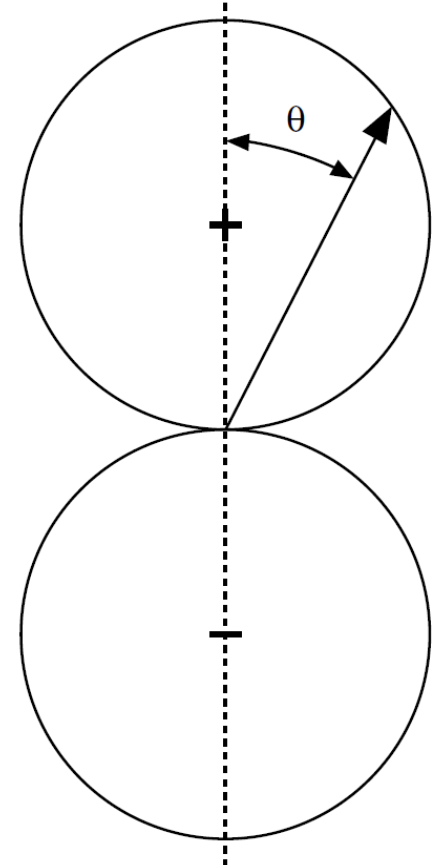
\includegraphics[width=0.2\textwidth]{images/5_8.png}
\end{figure}

The directional factor for a point dipole in the far field is given by:
\[
R(\theta) = \cos\theta.
\]

This directional dependence indicates that the dipole radiates most strongly along its axis and exhibits symmetry about its center. However, the radiation pattern also reveals a phase difference of \( 180^\circ \) between the two opposite directions. This means that the dipole emits sound waves in opposite directions with inverted phases.



\subsection{Quadrupole}

We can extend the concept of multiple sources by introducing a quadrupole, which can be modeled as a combination of two dipoles that effectively cancel each other out in certain directions. There are two configurations for quadrupoles: lateral quadrupoles and linear quadrupoles. Both configurations are composed of two dipoles, but their arrangements differ, resulting in distinct radiation patterns.

\begin{itemize}
    \item \textbf{Lateral Quadrupole}: The two dipoles are arranged side by side, with their axes perpendicular to each other. This results in a symmetric radiation pattern with four lobes of equal intensity, separated by regions of zero radiation in specific directions.
    \begin{figure}[H]
    \centering
    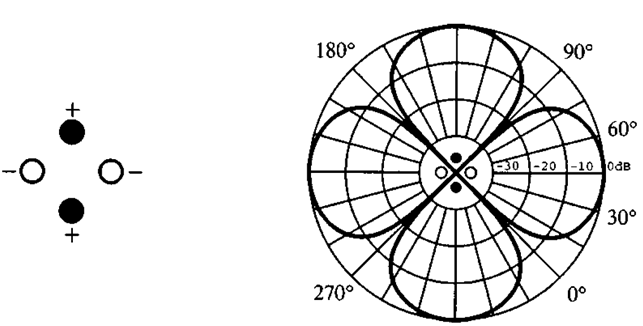
\includegraphics[width=0.5\textwidth]{images/5_9_1.png}
\end{figure}

\item \textbf{Linear Quadrupole}: The two dipoles are aligned along the same axis but oscillate with opposite phases. This creates a preferential axis of radiation with two main lobes of higher intensity and two weaker side lobes. The intensity distribution reflects the directional preference of the linear configuration.
    \begin{figure}[H]
    \centering
    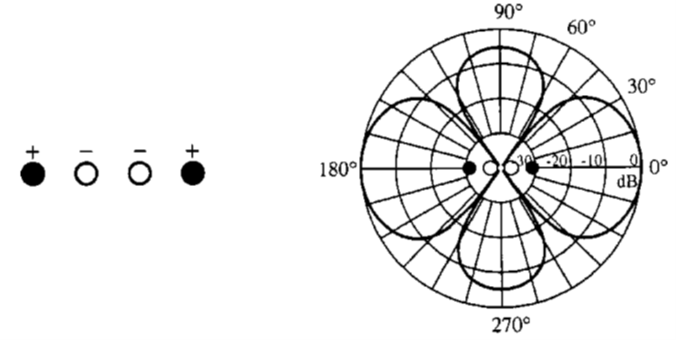
\includegraphics[width=0.5\textwidth]{images/5_9_2.png}
\end{figure}

\end{itemize}



A tuning fork provides a practical example of a linear quadrupole. The oscillating prongs of the fork produce forces that act on the surrounding medium. When the two prongs oscillate in opposite directions within the plane of the fork, the resulting radiation pattern resembles that of a linear quadrupole. 
For this analysis, we assume the quadrupole is a point quadrupole, meaning its physical size is significantly smaller than the wavelength of the radiated sound. For example, consider a tuning fork oscillating at \( f = 440 \, \text{Hz} \) (A4). The corresponding wavelength is approximately \( \lambda = 78 \, \text{cm} \). Since the dimensions of the tuning fork are much smaller than \( \lambda \), the point quadrupole approximation holds.    \begin{figure}[H]
    \centering
    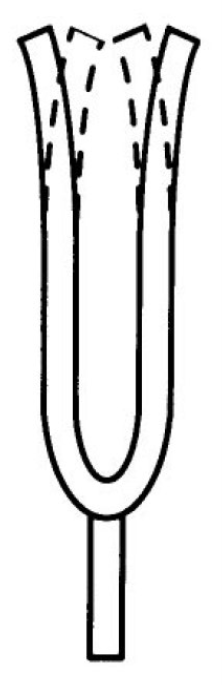
\includegraphics[width=0.1\textwidth]{images/5_9_3.png}
\end{figure}




\subsection{Linear Array}

When analyzing a linear array of \( N \) sources separated by a uniform distance \( d \), the objective is to determine the angular radiation pattern \( R(\alpha) \). This setup is particularly relevant in applications where control of the radiation pattern is essential, such as in audio and antenna arrays.
\begin{figure}[H]
    \centering
    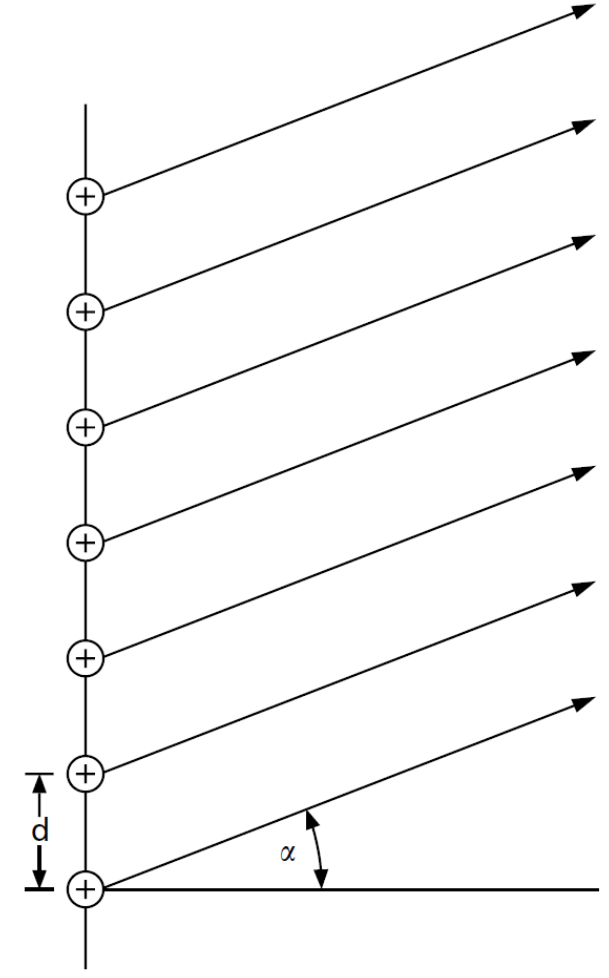
\includegraphics[width=0.3\textwidth]{images/5_10.png}
\end{figure}


In the far-field approximation, the radiated waves from all sources are considered parallel. The path difference between the waves emitted by two consecutive sources is given by:
\[
\Delta r = d \sin \alpha,
\]
where \( \alpha \) is the angle between the direction of propagation and the normal to the array.

The corresponding phase difference due to this path difference is:
\[
\Delta \phi = k d \sin \alpha, \quad \text{where } k = \frac{2\pi}{\lambda}.
\]

The total pressure field at a point \( P \) in the far field is the sum of contributions from all \( N \) sources. For the \( n \)-th source, the additional phase due to the path difference is \( n \Delta \phi = n k d \sin \alpha \). Thus, the total pressure field can be written as:
\[
p(r, \alpha, t) = \frac{j \omega \rho_0 \hat{Q}}{4 \pi r} \sum_{n=0}^{N-1} e^{j k d n \sin \alpha} e^{j (\omega t - kr)}.
\]

To simplify this expression, we use the formula for the sum of a geometric series:
\[
\sum_{n=0}^{N-1} q^n = \frac{1 - q^N}{1 - q}, \quad \text{where } q = e^{j k d \sin \alpha}.
\]
Substituting \( q \) into the pressure expression yields:
\[
p(r, \alpha, t)  = \frac{j \omega \rho_0 N \hat{Q}}{4 \pi r} \cdot \frac{e^{j N k d \sin \alpha} - 1}{N \left( e^{j k d \sin \alpha} - 1 \right)} \cdot e^{j (\omega t - k r)}.
\]

The directional factor \( R(\alpha) \), which modulates the intensity based on the angle \( \alpha \), is therefore:
\[
R(\alpha) = \frac{e^{j N k d \sin \alpha} - 1}{N \left( e^{j k d \sin \alpha} - 1 \right)} = \frac{\sin \left( N k d \sin \alpha / 2 \right)}{N \sin \left( k d \sin \alpha / 2 \right)}.
\]




The nature of the radiation pattern is determined by the relationship between the distance \( d \) and the wavelength \( \lambda \). 

By systematically analyzing \( R(\alpha) \), we identify maxima and minima in the intensity distribution.

The maxima occur when the denominator of \( R(\alpha) \) approaches zero, which happens when:
\[
\frac{k d}{2} \sin \alpha = m \pi, \quad m \in \mathbb{Z}.
\]
This implies that the angular positions of the maxima satisfy:
\[
\sin \alpha = \frac{2mp}{kd} = \frac{m \lambda}{d}.
\]
The condition \( |\sin \alpha| \leq 1 \) restricts the allowable values of \( m \), thereby defining the number of maxima visible in the pattern. When \( d < \lambda \), only \( m = 0 \) satisfies this condition, resulting in a single main lobe. However, as \( d > \lambda \), additional maxima appear at angles corresponding to \( m = \pm 1, \pm 2, \ldots \).

The minima, on the other hand, correspond to the points where the numerator of \( R(\alpha) \) vanishes. This condition is expressed as:
\[
\frac{N k d}{2} \sin \alpha = m' \pi \quad \to \quad \sin \alpha = \frac {m' {\lambda}}{ Nd}, \quad m' \in \mathbb{Z}.
\]
To avoid overlapping with maxima, \( m' \neq 0, \pm N \). 

Between two primary maxima, there are \( N - 1 \) minima and \( N - 2 \) secondary maxima. While the total number of primary maxima depends on the ratio \( \lambda / d \), the number of minima and secondary maxima is determined by the number of sources \( N \). 

The angular width of the main lobe is a critical parameter in characterizing the directionality of the array. It is conventionally defined as the angular separation between the first minima on either side of the main lobe. The first minima occur at:
\[
\sin \alpha = \pm \frac{\lambda}{N d}.
\]
Thus, the angular width is given by:
\[
\Delta \alpha \approx \Delta \sin \alpha = \frac{2 \lambda}{N d}.
\]
This shows that the width of the main lobe decreases as \( N \) increases, enhancing the array's directionality.

The intensity at the maxima scales with \( N^2 \), so the intensity of maxima depends on the number of sources, while the angular positions of the maxima  depend solely on \( \lambda / d \), meaning that the position of maxima does not depend on the number of sources. This behavior underscores the trade-off between angular resolution and array complexity: increasing \( N \) narrows the main lobe, providing higher angular resolution at the expense of additional sources.\\



To analyze the radiated power, we consider two configurations of sources: one forming a dipole with \((- +)\) phase relationship, and another forming an array with all sources in phase (\(+ +\)). The radiated power is studied as a function of the relative distance between the sources, expressed in terms of \(kd\), for a given wavelength. 
\begin{figure}[H]
    \centering
    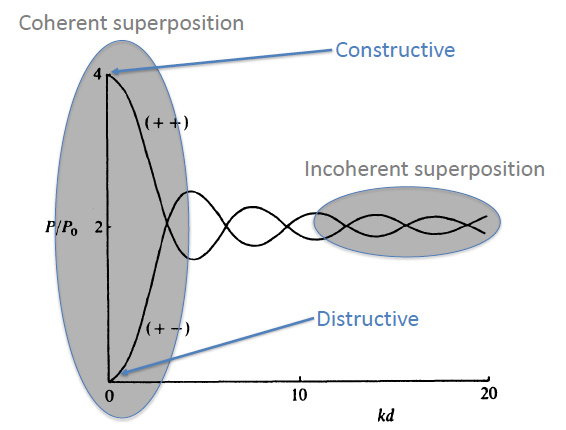
\includegraphics[width=0.6\textwidth]{images/5_11_2.png}
\end{figure}

We assume that each individual source radiates a power \(P_0\). At \(kd = 0\), when the sources overlap perfectly, the radiated power depends on their phase relationship. In the case of a \((+-)\) configuration (dipole), the sources are out of phase, and their contributions cancel each other completely, resulting in zero radiation. This cancellation is not due to traditional interference but rather an intrinsic annihilation caused by their opposing phases. Conversely, in the \((++)\) configuration, where the sources are in phase, their overlap produces constructive superposition, resulting in maximum radiated power (4 times the power of a single source). 

In the case of a point dipole, where the two sources are very close to each other (\(kd \ll 1\)), the radiated power is minimal due to their destructive interaction. This is consistent with the weak radiation pattern expected from a point dipole.




For coherent superposition, the relative phase between the sources plays a significant role: a \((+ +)\) configuration behaves entirely differently from a \((+ -)\) configuration at small separations. However, as the sources become very distant from each other (\(kd \gg 1\)), the overall radiated power of both configurations (\(+ -\) and \(+ +\)) tends to converge to similar levels, as the effect of their phase relationship diminishes over large separations.\\


In an array of \( N \) sources, each monopole can possess its own initial phase. This concept leads us to the definition of a \textbf{phased array}, which is a linear arrangement of antennas or sources where the phase of each source is controlled independently. By adjusting these phases, we can steer the direction of constructive interference in space, effectively directing the emitted radiation or sound to a desired angle.

The pressure field for such an array, incorporating the initial phase of each monopole, is expressed as:
\[
p(r, \alpha, t) = \frac{j \omega \rho_0 \hat{Q}}{4 \pi r} \sum_{n=0}^{N-1} e^{j k d n \sin \alpha} \cdot e^{j (\omega t - k r)} e^{j \phi_n},
\]
where \( \phi_n \) is the initial phase assigned to the \( n \)-th source.

The conditions for constructive and destructive interference now depend on both the difference in path lengths and the initial phase differences. By manipulating the phases \( \phi_n \), we can beam the sound or electromagnetic waves in specific directions without physically moving the sources. This technique finds extensive applications, such as in loudspeaker systems and antenna arrays for telecommunications.

The three diagrams here illustrate different radiation patterns achieved by varying the distances and phases between the sources:
\begin{figure}[H]
    \centering
    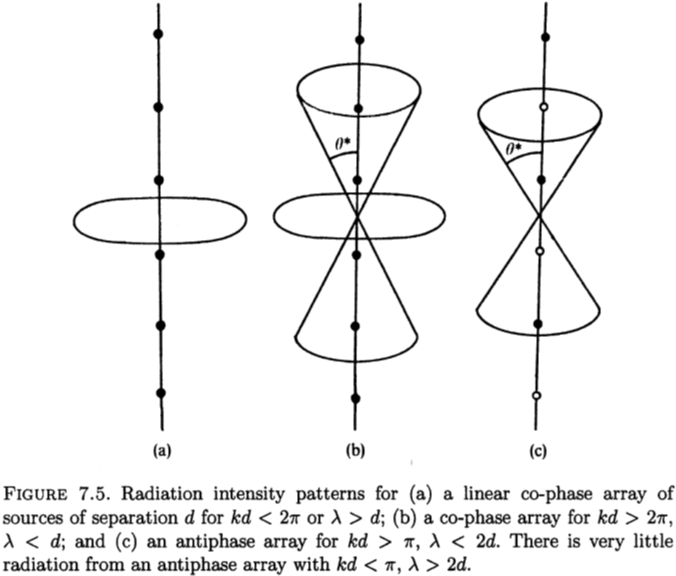
\includegraphics[width=0.6\textwidth]{images/5_12.png}
\end{figure}

\begin{itemize}
    \item Linear Co-Phase Array with Small Distance (\( kd < 2\pi \)): When the distance between the sources is small and all are in phase, a single maximum occurs in the equatorial plane, with no additional maxima elsewhere. The radiation is concentrated in a single direction.

\item Co-Phase Array with Larger Distance (\( kd > 2\pi \)): Increasing the distance between sources introduces additional maxima in the radiation pattern, leading to multiple directions of emission. The lobes become more prominent as the distance increases.

\item Anti-Phase Array (\( \phi = 180^\circ \)): By setting a 180° phase difference between alternating sources (\( +- \)), we eliminate the maximum in the equatorial plane and instead retain maxima along the axis. This configuration demonstrates the capability of phased arrays to suppress unwanted directions of radiation while emphasizing others.
\end{itemize}

Through these examples, we see how phase and distance can be manipulated to tailor the radiation pattern, enabling precise control over the direction and intensity of the emitted waves.


\subsection{Directional factor}

In this example, we analyze the three-dimensional radiation pattern of a \textbf{loudspeaker array}. The distance from the center of the plot represents the intensity of the sound, where red regions correspond to higher intensity and blue regions to weaker intensity. This visualization provides insight into how the arrangement of loudspeakers and the frequency of the signal influence the angular distribution of sound.
\begin{figure}[H]
    \centering
    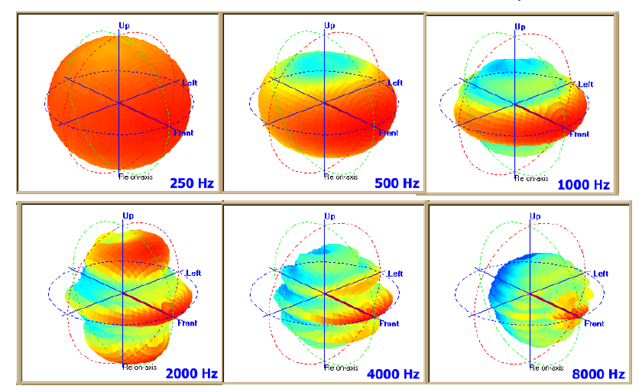
\includegraphics[width=0.7\textwidth]{images/5_13.png}
\end{figure}

For a given configuration of loudspeakers, the behavior of the emitted sound changes depending on the frequency, which determines the wavelength (\( \lambda \)). When the wavelength is much larger than the distance \( d \) between the loudspeakers, the emission appears isotropic. This means the sound intensity is evenly distributed in all directions. 

As the wavelength becomes comparable to the distance \( d \), the radiation pattern evolves, and distinct maxima start appearing along different directions. These maxima represent regions of constructive interference, as the loudspeakers are all driven by the same signal and are in phase. The number and angular positions of these maxima depend on the ratio \(  \lambda / d \), as derived earlier in the context of linear arrays.

The azimuthal (\( \phi \)) distribution is influenced by the geometry of the loudspeakers and the presence of components like horns, which can shape the horizontal emission pattern. However, the polar (\( \theta \)) distribution aligns closely with the theoretical predictions derived from the formulas studied earlier.

It is important to note that different frequencies result in different angular propagation characteristics. This frequency dependency poses challenges in large spaces where uniform sound diffusion is desired. Understanding and managing these radiation patterns is crucial for achieving consistent acoustic coverage in venues such as concert halls, theaters, and public spaces.\\




Now we simulate the polar emission pattern of a \textbf{single loudspeaker}. The speaker is modeled as an extended source composed of many infinitesimal point sources, forming a continuous array. Each point source radiates an infinitesimal amount of power, and the overall pattern results from the interference of all these contributions. 

When the size of the speaker \( d \) is much smaller than the wavelength \( \lambda \), the phase differences due to different path lengths from various parts of the speaker are negligible. In this scenario, the radiation pattern is isotropic, as all contributions effectively travel the same path. However, as the frequency increases and the wavelength becomes comparable to or smaller than \( d \), the path differences start to matter, leading to interference effects. The speaker then begins to behave as a complex source, with the radiation pattern becoming increasingly directional.

The simulation compares two speakers of different sizes (\( d = 5 \, \text{cm} \) and \( d = 25 \, \text{cm} \)) at various frequencies:

\begin{figure}[H]
    \centering
    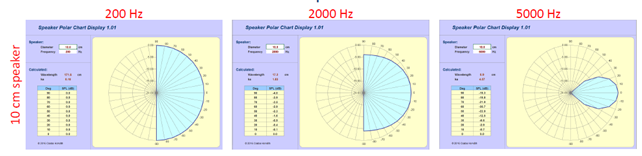
\includegraphics[width=0.9\textwidth]{images/5_14_1.png}
\end{figure}
\begin{figure}[H]
    \centering
    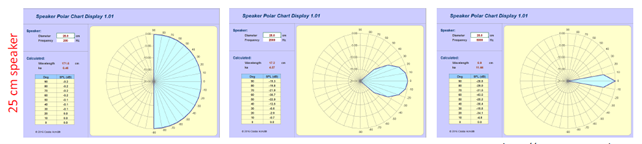
\includegraphics[width=0.9\textwidth]{images/5_14_2.png}
\end{figure}


For \( f = 200 \, \text{Hz} \) (\( \lambda \approx 1.7 \, \text{m} \)), both the \( d = 10 \, \text{cm} \) and \( d = 25 \, \text{cm} \) speakers behave as point sources, emitting isotropically. Since the size of the speakers is much smaller than the wavelength (\( d \ll \lambda \)), there is negligible interference and the radiation pattern remains uniform.

At \( f = 2000 \, \text{Hz} \) (\( \lambda \approx 0.17 \, \text{m} \)), the \( d = 10 \, \text{cm} \) speaker still exhibits nearly isotropic radiation but starts showing a slightly higher intensity in the equatorial plane. For the \( d = 25 \, \text{cm} \) speaker, interference effects become significant, and the radiation becomes more directional. This shift is due to the comparable size of the speaker to the wavelength, where \( d \sim \lambda \).

At \( f = 5000 \, \text{Hz} \) (\( \lambda \approx 0.069 \, \text{m} \)), the radiation pattern of the \( d = 10 \, \text{cm} \) speaker becomes slightly directional, while the \( d = 25 \, \text{cm} \) speaker exhibits a strongly directional pattern with pronounced lobes. The smaller wavelength causes more significant phase differences between contributions from different parts of the speaker, enhancing the interference effects.


In practice, these behaviors necessitate careful design of loudspeaker systems to ensure uniform angular response across the frequency spectrum. This is achieved by using speakers of different sizes for different frequency bands:
high frequencies are assigned to smaller speakers (\( d \approx 5 \, \text{cm} \)),
mid frequencies to medium-sized speakers (\( d \approx 10 \, \text{cm} \)),
low frequencies to larger speakers (\( d \approx 25 \, \text{cm} \)). By maintaining a consistent ratio \( \lambda / d \) for all speakers, the angular response remains balanced across the spectrum. This ensures that sound intensity and directionality are uniform, addressing the challenges of complex radiation patterns caused by frequency-dependent interference.

\subsection {Doppler Effect}

The Doppler effect describes the alteration of the perceived frequency when there is relative motion between the source of a sound and the observer. This phenomenon can be divided into two scenarios: one in which the source is moving relative to the observer, and another in which the observer is moving relative to the source. While velocity is relative and depends on the chosen reference frame, this problem involves three distinct entities: the source, the observer, and the medium in which the sound propagates. For both moving point sources and observers, the relative velocity is considered in the reference frame of the medium (typically a fluid such as air).

In the case of \textbf{moving point source}, when the source is moving towards the listener, the emitted wavelength is shortened.
\begin{figure}[H]
    \centering
    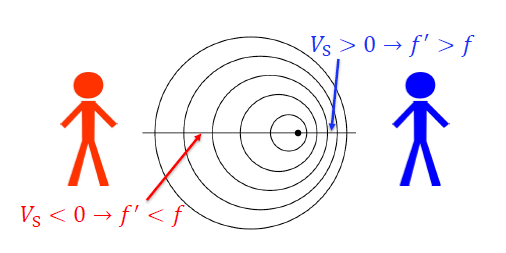
\includegraphics[width=0.5\textwidth]{images/5_15_1.png}
\end{figure}
This is because the source emits consecutive wavefronts at intervals of its oscillation period \( T \), but its movement compresses the distance between the wavefronts. The new wavelength can be calculated as:
\[
\lambda' = (c - V_s)T,
\]
where \( V_s \) is the velocity of the source, \( c \) is the speed of sound, and \( T \) is the oscillation period. The corresponding perceived frequency \( f' \) is then:
\[
f' = \frac{f}{1 - \frac{V_s}{c}},
\]
where \( f \) is the frequency of the source in the absence of motion.

In the case of a \textbf{moving observer}, the apparent frequency change is due to the variation in the time interval between successive wavefronts reaching the observer. 
\begin{figure}[H]
    \centering
    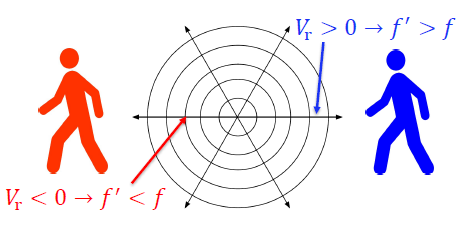
\includegraphics[width=0.5\textwidth]{images/5_15_2.png}
\end{figure}

Here, the perceived frequency is given by:
\[
f' = \frac{C + V_r}{\lambda} = \left( 1 + \frac{V_r}{c} \right)f,
\]
where \( V_r \) is the velocity of the observer relative to the medium.

While these two scenarios yield different equations, they are quantitatively similar when the relative velocity is much smaller than the speed of sound. For instance, if the velocity \( V_s \) or \( V_r \) is 1\% of \( c \), the frequency shift is approximately 1\% of the original frequency. The distinction lies in the qualitative interpretation: in the first case, the wavelength is altered, while in the second case, the time interval between received wavefronts changes.

The Doppler effect has an intriguing musical application in devices like the Leslie speaker, where the relative motion between a sound source and a listener is exploited to create dynamic frequency modulations, enhancing the auditory experience.


\section{Extended sources, Reflection and refraction, Diffraction and Scattering}



In this section, we transition from the point source approximation to extended sources. These extended sources are analyzed as continuous distributions of infinitesimal point sources. Subsequently, we will explore the interaction between waves and objects, delving into the effects of scattering and interference.

\subsection{Pulsating Sphere}

The primary distinction in this analysis is that the source is no longer approximated as a point compared to the wavelength. This means the source's radius \( R \) is significant, potentially comparable to or larger than the wavelength \( \lambda \). This necessitates revisiting the pressure field and recasting the expressions to account for the finite size of the source.


\begin{figure}[H]
    \centering
    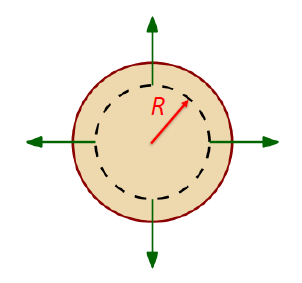
\includegraphics[width=0.3\textwidth]{images/6_3.png}
\end{figure}



For a spherical source with radius \( R \), the velocity field at the surface is given by:

\[
v_r(R, t) = u e^{j\omega t} = \frac{p(R, t)}{\rho_0 c} \left( 1 + \frac{1}{j k R} \right).
\]

From this relationship, the pressure field at the surface of the source is expressed as:

\[
p(R, t) = \rho_0 c u e^{j \omega t} \left( 1 - \frac{j}{k R} \right).
\]

On the other hand, the pressure field for a spherical wave is given by:

\[
p(R, t) = \frac{A}{R} e^{j (\omega t - k R)}.
\]

Equating the two expressions for \( p(R, t) \), we have:

\[
\frac{A}{R} e^{j (\omega t - k R)} = \rho_0 c u e^{j \omega t} \left( 1 - \frac{j}{k R} \right).
\]

By isolating \( A \), multiplying through by \( R \), and reorganizing terms, we get:

\[
A e^{-j k R} = \rho_0 c R u \left( 1 - \frac{j}{k R} \right).
\]

Finally, factoring \( 1 - j k R \) and normalizing by \( 1 + k^2 R^2 \), the expression for \( A \) becomes:

\[
A = j \rho_0 c k R^2 u \cdot \frac{1 - j k R}{1 + k^2 R^2} e^{j k R}.
\]



The pressure at any point in the field, taking into account the finite size of the source, is then given by:
\[
p(r, t) = \frac{A}{r} e^{j (\omega t - k r)} = \frac{j \rho_0 c k R^2 u}{r} \cdot \frac{1 - j k R}{1 + k^2 R^2} e^{j [\omega t - k (r - R)]}.
\]




We have previously expressed the pressure wave as a function of volume velocity \( Q(t) \), but now we analyze the radiated power, a key parameter in characterizing sound sources. To analyze the radiated power, we focus on a regime where the observation distance is much larger than the size of the source (\( r \gg R \)), ensuring power conservation over different distances. Additionally, we consider a source with a radius much smaller than the wavelength (\( R \ll \lambda \)), which reflects a typical situation for many musical instruments, where the size of the emitting volume is small compared to the wavelength of the radiated sound. Under these conditions (\( kR \ll 1 \)), we can neglect terms involving \( R \) and simplify the pressure expression for the far field.

\[
p(r, t) = \frac{j \rho_0 c k R^2 u}{r} e^{j(\omega t - kr)} \quad \text{where} \quad A =  j \rho_0 c k R^2 u
\]

Substituting \(A\) in the intensity expression for a spherical wave:
\[
\overline{I} = \frac{1}{2} \frac{A^2}{\rho_0 c r^2} 
 = \frac{1}{2} \frac{\left(j \rho_0 c k R^2 u \right)^2}{\rho_0 c r^2} = \frac{\rho_0 c k^2 R^4 u^2}{2 r^2}.
\]

The total radiated power, \( \overline{P} \), is then obtained by integrating the intensity over the surface of a sphere:

\[
\overline{P} = \int_{S}\overline{I} \, dS = 4\pi r^2 \overline{I} = 2 \pi \rho_0 c k^2 R^4 u^2.
\]

This result shows that the radiated power of a small spherical source scales with the fourth power of its radius (\( \overline{P} \propto R^4 \)) and with the square of the frequency (\( \overline{P} \propto k^2 \propto \omega^2 \)).



The scaling of radiated power with \( R^4 \) highlights the inefficiency of very small sources in radiating waves whose wavelength is much larger than their size.  For very small sources, radiated power is inefficient because their size prevents effective coupling with the wavelength of the wave. As the source size increases and becomes comparable to the wavelength, the coupling improves, significantly enhancing power radiation. In summary, to efficiently emit or receive waves, the size of the source must not be much smaller than the wavelength. This principle underscores why molecules, for example, are inefficient emitters of light: their size is thousands of times smaller than the wavelength of the light they try to emit. This principle also applies to antennas: a small antenna, whose dimensions are much smaller than the wavelength of the electromagnetic wave it attempts to emit or receive, will be inefficient. To overcome this, antennas are designed to have dimensions comparable to the wavelength, thereby enhancing their effectiveness, enabling efficient energy transfer.

Additionally, the proportionality to \( k^2 \) (\( \omega^2 \)) implies an inherent frequency response. High frequencies, which correspond to shorter wavelengths, are radiated more efficiently. Conversely, low frequencies are suppressed, particularly for small sources. For monopole sources, the radiated power scales with \( k^2 \) (as the pressure scales with \( k \)), while for dipole sources, it scales with \( k^4 \) (as the pressure scales with \( k^2 \). This indicates that dipole sources are even less efficient at radiating low frequencies compared to monopole sources. Moreover, this difference in scaling reveals a distinct frequency response between monopole and dipole sources. Dipoles tend to suppress low frequencies more significantly, making their radiation spectrum qualitatively different.



\subsection{Line Sources}

Line sources represent continuous distributions of sound-emitting points along a line. This model is particularly useful for describing physical systems such as vibrating cylinders, where the lateral surface expands and contracts radially. Our goal is to calculate the pressure wave at a specific observation point \( P \) in space.
\begin{figure}[H]
    \centering
    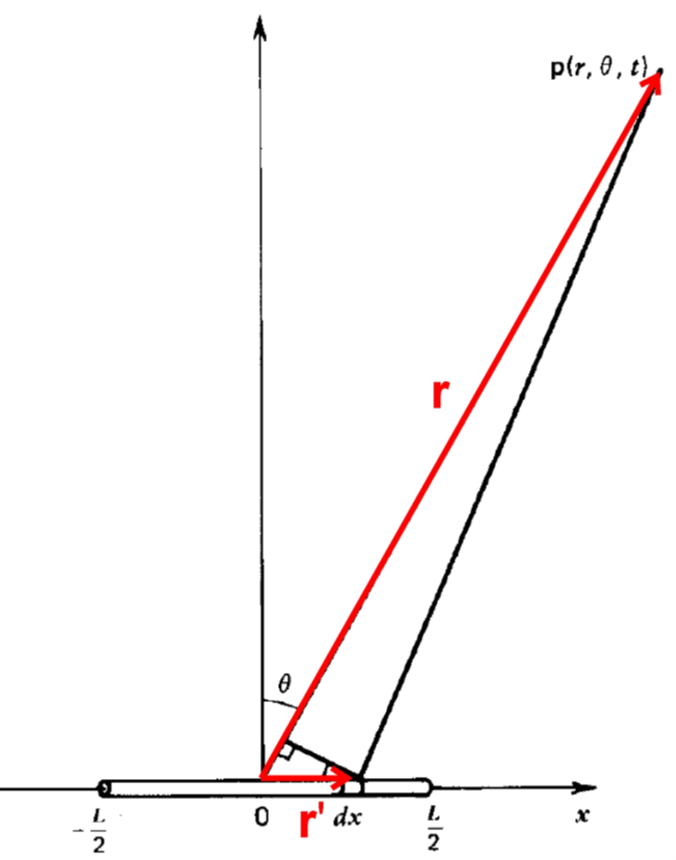
\includegraphics[width=0.4\textwidth]{images/6_5.png}
\end{figure}
A line source is modeled as having a finite length \( L \), and the observation point \( P \) is described in a cylindrical coordinate system by two parameters: the distance \( r \) from the center of the source and the angle \( \theta \) with respect to the cylinder's axis. Each infinitesimal segment of the line source, with length \( dx \), is treated as an infinitesimal monopole, generating a spherical wave that contributes to the pressure field at \( P \). To determine the total pressure wave at \( P \), it is necessary to integrate all contributions along the length of the line source. This formulation inherently involves solving an interference problem, as contributions from all parts of the source must be summed with their respective amplitudes and phases.

The infinitesimal volume velocity \( dQ \) associated with each segment \( dx \) depends on the surface velocity \( u \) and the surface area element \( dS \) of the cylindrical source. The surface area of an infinitesimal cylindrical segment is expressed as \( dS = 2 \pi R \, dx \), where \( R \) is the radius of the cylinder. Consequently, the volume velocity for an infinitesimal segment becomes:
\[ Q(t) = \frac{dV}{dt} = u \, S \quad \to \quad
dQ = u \, dS = U_0 e^{j\omega t} \cdot 2 \pi R \, dx,
\]
where \( u = U_0 e^{j\omega t} \) represents the harmonic oscillation of the surface velocity.

The pressure contribution \( dp(r) \) at the observation point \( P \), due to the infinitesimal segment \( dx \), is given by:
\[
dp(r) = \frac{\rho_0 j \omega dQ}{4 \pi |r - r'|} e^{-j k |r - r'|} e^{j \omega t},
\]
where \( |r - r'| \) is the distance between the observation point \( P \) and the segment \( dx \), and \( k = \frac{2 \pi}{\lambda} \) is the wavenumber. Substituting the expression for \( dQ \), we obtain:
\[
dp(r) = \frac{\rho_0 j \omega U_0 R}{2} \frac{e^{-j k |r - r'|}}{|r - r'|} dx \, e^{j \omega t}.
\]

To compute the total pressure at the observation point, the contributions from all infinitesimal segments of the line source must be integrated:
\[
p(r, t) = \frac{\rho_0 j \omega U_0 R}{2} e^{j \omega t} \int_{-L/2}^{L/2} \frac{e^{-j k |r - r'|}}{|r - r'|} dx.
\] \\



To analyze the far-field behavior of the pressure wave generated by a line source of length \( L \), we assume the condition \( r \gg L \), so that \( |r - r'| \) and \( r \) are parallel. This assumption simplifies the mathematical treatment by allowing approximations for both the amplitude and the phase terms of the pressure wave.
The distance \( |r - r'| \), which appears in the phase term \( e^{-j k |r - r'|} \), can be approximated as:
\[
|r - r'| \approx r - x \sin \theta,
\]

This substitution is made because, in the phase term, every tiny difference matters significantly when compared to the wavelength. The term \( x \sin \theta \), even if small, can have a large impact on the phase due to its relationship with the wavelength \( \lambda \). As long as \( x \sin \theta \) is not negligible compared to \( \lambda \), its effect on the phase cannot be ignored.

However, in the denominator \( |r - r'| \), the variations in \( r' \) are much smaller than \( r \). Since the denominator acts as a multiplicative factor affecting the amplitude rather than the phase, these small differences can be neglected. This leads to the approximation:
\[
\frac{1}{|r - r'|} \approx \frac{1}{r}.
\]



Applying these approximations, the pressure field becomes:
\[
p(r, t) = \frac{j \omega \rho_0 U_0 R}{2 r} e^{j (\omega t - k r)} \int_{-L/2}^{L/2} e^{-j k x \sin \theta} \, dx.
\]

The integral term accounts for the interference between contributions from different points along the line source. Solving this integral yields:
\[
\int_{-L/2}^{L/2} e^{-j k x \sin \theta} \, dx = \frac{\sin \left( \frac{1}{2} k L \sin \theta \right)}{\frac{1}{2} k L \sin \theta}.
\]

Substituting back, the final expression for the pressure wave in the far-field is:
\[
p(r, t) = \frac{j \omega \rho_0 U_0 R L}{2 r} \cdot \frac{\sin \left( \frac{1}{2} k L \sin \theta \right)}{\frac{1}{2} k L \sin \theta} e^{j (\omega t - k r)}.
\]

This result consists of two main components:
\begin{itemize}
    \item Amplitude: \(\frac{j \omega \rho_0 U_0 R L}{2 r}\), which describes the decay of the wave with distance \( r \).
\item Directional factor: \(\frac{\sin \left( \frac{1}{2} k L \sin \theta \right)}{\frac{1}{2} k L \sin \theta}\), which defines the angular distribution of the radiated pressure. This factor demonstrates that the radiation pattern depends on the angle \( \theta \), with constructive and destructive interference shaping the directional characteristics.
\end{itemize}



The radiation pattern of a line source is very similar to the one of a linear array of discrete sources. By plotting the directional factor, the first zero occurs when:

\[
\frac{1}{2} k L \sin \theta = \pi \implies \sin \theta = \frac{\lambda}{L}.
\]

This relationship highlights the dependence of the angular position of the first null on the length \( L \) of the line source. As the length \( L \) increases, the angle \( \theta \) of the first null becomes smaller, leading to a narrower main lobe. Thus, the radiation pattern becomes increasingly directional with longer line sources.

\begin{figure}[H]
  \centering
  \begin{minipage}{0.5\textwidth}
    \centering
    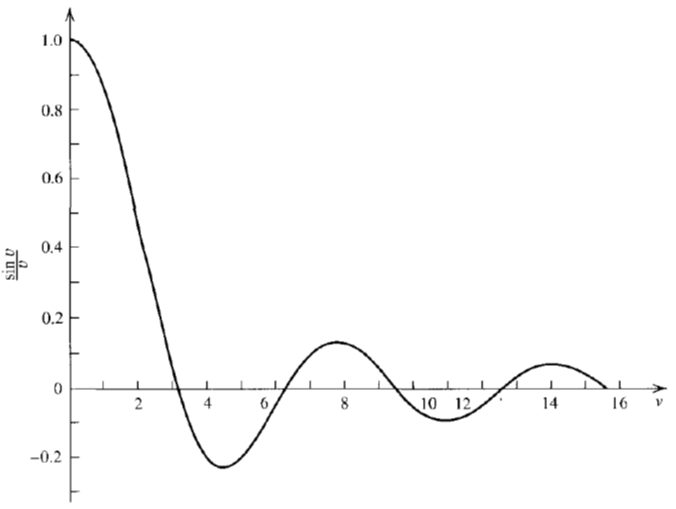
\includegraphics[width=\textwidth]{images/6_7_1.png}
  \end{minipage}%
  \hfill
  \begin{minipage}{0.4\textwidth}
    \centering
    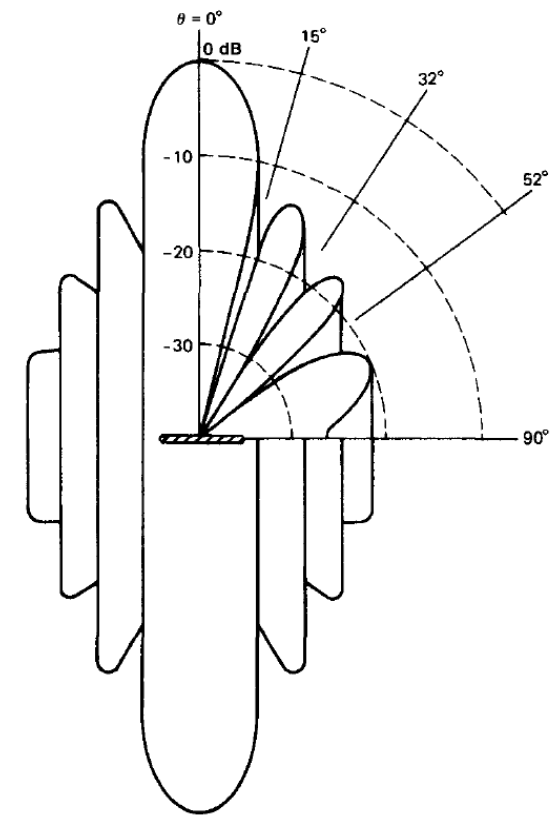
\includegraphics[width=\textwidth]{images/6_7_2.png}
  \end{minipage}
\end{figure}

\subsection{Plane Source}
The radiation from a plane source can be understood as a model mimicking the radiation from any vibrating source. In this case, the source is a baffled plane source. To illustrate this, let us consider a loudspeaker that is not enclosed in a case. Without a baffle, the piston of the loudspeaker moves back and forth, behaving like a dipole. However, a dipole is an inefficient source: it performs poorly at radiating low frequencies (its spectral response is not ideal) and is generally inefficient in radiating power. The backward radiation from such a source typically bounces off nearby walls, interferes with the primary forward sound, and creates unwanted effects. 

To address these issues, the loudspeaker is often enclosed in a box or baffle. This configuration suppresses the backward radiation, transforming the dipole into a monopole source. However, the baffle limits the radiation to half-space, reducing the total radiated power to half of what a monopole radiating in free space would emit. Thus, a baffle can be seen as a collection of monopoles radiating exclusively into half-space.

\begin{figure}[H]
  \centering
  \begin{minipage}{0.3\textwidth}
    \centering
    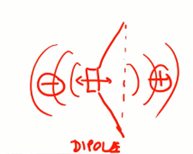
\includegraphics[width=\textwidth]{images/6_8_1.png}
  \end{minipage}%
  \hfill
  \begin{minipage}{0.2\textwidth}
    \centering
    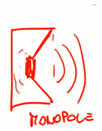
\includegraphics[width=\textwidth]{images/6_8_2.png}
  \end{minipage}
\end{figure}

To describe this mathematically, consider the active surface of the baffle with a specific surface area and volume velocity. Each infinitesimal element \( dS \) of the active surface can be treated as an infinitesimal monopole, contributing to the total pressure wave. The volume velocity of the source depends on the position and can be expressed as \( u(r') \), where \( r \) points to the observation point where the pressure wave is calculated, and \( r' \) is the integration vector pointing toward an infinitesimal source element.

\begin{figure}[H]
    \centering
    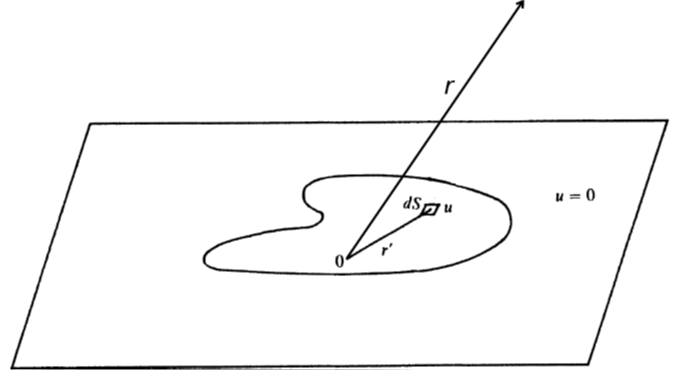
\includegraphics[width=0.6\textwidth]{images/6_8.png}
\end{figure}

The infinitesimal volume velocity, \( dQ \), is given by:
\[
dQ = u(r') dS,
\]
and each infinitesimal volume velocity generates an infinitesimal spherical wave. The pressure contribution at a point \( r \) due to an element \( dS \) is:
\[
dp(r) = \frac{j \omega \rho_0}{2 \pi} \frac{e^{-j k |r - r'|}}{|r - r'|} u(r') dS,
\]
where the denominator includes the factor \( 2 \pi \) because the baffle confines the radiation to half-space.

To calculate the total pressure wave \( p(r) \), the contributions from all the infinitesimal elements are integrated over the entire surface \( S \):
\[
p(r) = \frac{j \omega \rho_0}{2 \pi} \iint_S \frac{e^{-j k |r - r'|}}{|r - r'|} u(r') dS.
\]

\subsection{Plane Circular Piston}

For a circular piston, which serves as an idealized approximation for a loudspeaker, the pressure field at a point in space can be determined by solving the integral over the surface of the piston. In this case, \( dS \) represents the infinitesimal source element on the vibrating piston surface. 

We assume the velocity of all points on the piston surface to be uniform, meaning the piston vibrates harmonically with the same velocity amplitude \( U_0 \), which is described by:
\[
u = U_0 e^{j \omega t}.
\]

The total pressure wave \( p(r, t) \) at an observation point \( r \) is given by the integration of the contributions from each infinitesimal source element \( dS \). Substituting the uniform velocity \( u \) into the general expression for the pressure wave, we obtain:
\[
p(r, t) = \frac{j \omega \rho_0}{2 \pi} \iint_S \frac{e^{-j k |r - r'|}}{|r - r'|} u dS  = \frac{j \omega \rho_0 U_0 e^{j \omega t}}{2 \pi} \iint_S \frac{e^{-j k |r - r'|}}{|r - r'|} dS.
\]


The listener is located at a point \( p \) directly in front of the loudspeaker, which corresponds to the axis of symmetry (\( \theta = 0 \)). 
\begin{figure}[H]
    \centering
    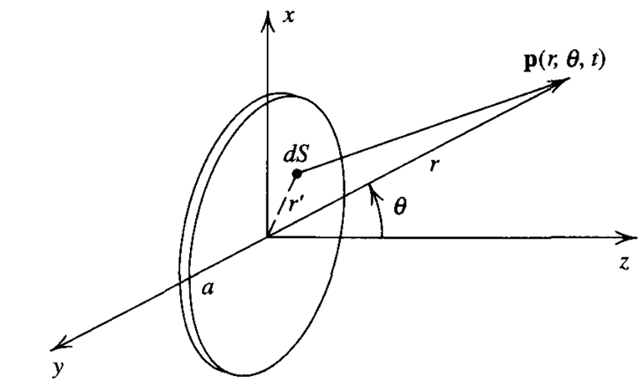
\includegraphics[width=0.6\textwidth]{images/6_9.png}
\end{figure}

The integration simplifies due to the axial symmetry of the problem. All points on the piston at the same radial distance \( r' \) from the center contribute equally to the pressure field at \( p \). Thus, instead of considering individual infinitesimal sources \( dS \) arbitrarily distributed across the surface, we take advantage of the symmetry to define the infinitesimal source area \( dS \) as a ring of radius \( r' \) and thickness \( dr' \). The area of such a ring is given by:
\[
dS = 2\pi r' dr'.
\]
\begin{figure}[H]
  \centering
  \begin{minipage}{0.45\textwidth}
    \centering
    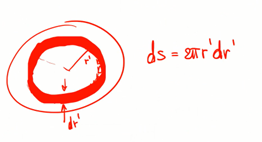
\includegraphics[width=\textwidth]{images/6_10_1.png}
  \end{minipage}%
  \hfill
  \begin{minipage}{0.3\textwidth}
    \centering
    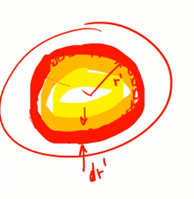
\includegraphics[width=\textwidth]{images/6_10_2.png}
  \end{minipage}
\end{figure}

This approach reduces the problem to a single variable of integration (\( r' \)), making the computation more efficient. Each of these infinitesimal sources contributes a pressure wave to the overall field. As shown in the derivation, the pressure field at the axial point \( p \) can be expressed as:
\[
p(r, t) = \frac{j\omega \rho_0 U_0 e^{j\omega t}}{2\pi} \int_0^a \frac{e^{-jk\sqrt{r^2 + r'^2}}}{\sqrt{r^2 + r'^2}} 2\pi r' dr',
 = j \omega \rho_0 U_0 e^{j\omega t} \left[ \frac{e^{-jk\sqrt{r^2 + r'^2}}}{jk} \right]_0^a =
\]
\[
= c \rho_0 U_0 e^{j\omega t} \left( e^{-jkr} - e^{-jk\sqrt{r^2 + a^2}} \right)
= c \rho_0 U_0 \left( 1 - e^{-jk(\sqrt{r^2 + a^2} - r)} \right) e^{j(\omega t - kr)}.
\]
where \( a \) is the radius of the piston, and the integration accounts for all the infinitesimal contributions from each ring on the surface of the piston.
 \begin{figure}[H]
    \centering
    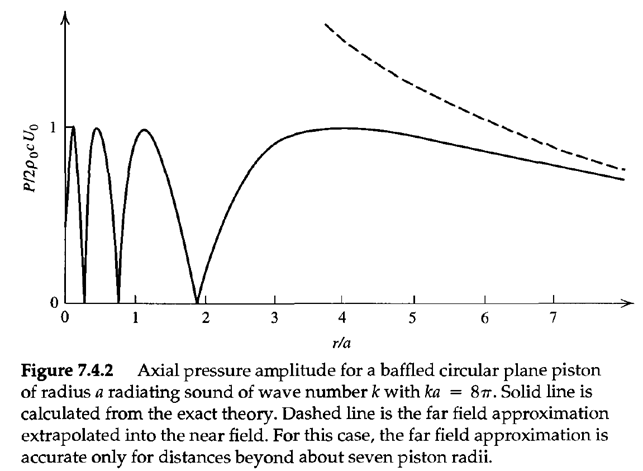
\includegraphics[width=0.6\textwidth]{images/6_11.png}
\end{figure}
The graph shows the axial pressure amplitude as a function of \( r/a \), where \( a \) is the piston radius. The pressure wave generated by a baffled circular plane piston decays as a function of the distance \( r \). This decay behavior is influenced significantly in the near field, where the distance is comparable to the size of the speaker (radius \( a \)). In the near field, the pressure field exhibits complex constructive and destructive interference effects due to the contributions from various regions of the piston. This makes the near-field region highly irregular and not suitable for practical use, especially for applications requiring uniform radiation patterns.\\

When we consider the sound pressure field generated by a baffled circular piston source, moving away from the axis of symmetry requires additional complexity in the mathematical formulation. Along the axis, we had a simplified scenario, but as we deviate from the axis, the integral formulation becomes more involved. 
 \begin{figure}[H]
    \centering
    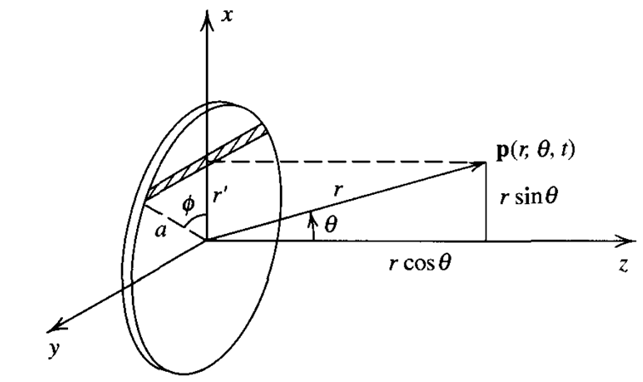
\includegraphics[width=0.6\textwidth]{images/6_12.png}
\end{figure}

\[
dp(r, t) = \left( \frac{j \omega \rho_0 U_0 R L}{2 |r - r'|} \right) 
\left( \frac{\sin \left( \frac{1}{2} k L \sin \theta \right)}{\frac{1}{2} k L \sin \theta} \right) 
e^{j \left( \omega t - k |r - r'| \right)}
\]

For points away from the axis, we use the far-field approximation to simplify the analysis ( \(r \gg a \) ). In the far field, the exact solution aligns closely with the far-field approximation. However, in the near field, significant deviations arise due to interference effects.

To analyze the sound field off-axis, we consider an alternative approach to reduce the complexity of the system. Specifically, we divide the circular surface into an infinite collection of linear sources. Each linear source has a thickness \( R \, dx \), and its length \( L \) can be expressed as \( 2a \sin \phi \), where \( a \) is the radius of the circular piston, and \( \phi \) is the angular position. In the far-field regime, we assume \( r - r' \approx r \) in the amplitude terms, and \( \theta \) is small. However, in the exponential phase term \( e^{-j k |r - r'|} \), the correction factor due to the distance variation is critical, represented as \( x \sin \theta \cos \phi \). 

To determine the pressure field generated by the entire plane circular piston, we consider the contribution of all infinitesimal sources on the piston surface: 
\[
p(r, t) = \frac{j \omega \rho_0 U_0 R a}{r} e^{j (\omega t - k r)} 
\int_{-a}^{a} e^{-j k x \sin \theta \cos \phi} \sin \phi \, dx
= \frac{j \omega \rho_0 U_0 R a}{r} e^{j (\omega t - k r)} 
\int_{0}^{\pi} e^{-j k x \sin \theta \cos \phi} \sin^2 \phi \, d\phi

\]


This integral, however, cannot be solved analytically due to its complexity. Instead, we employ the first-order Bessel function of the first kind \( J_1 \) to express the solution:
\[
p(r, t)  = \frac{j \omega \rho_0 U_0 R a^2}{2 r} \left[ \frac{2 J_1(k a \sin \theta)}{k a \sin \theta} \right] e^{j(\omega t - k r)}.
\]
Here:
\begin{itemize}
    \item  \( J_1 \) is the Bessel function of the first kind of order one.
\item The term \( \frac{2 J_1(k a \sin \theta)}{k a \sin \theta} \) represents the directional factor, showing how the sound field changes with the angle \( \theta \).
\item The amplitude term \( \frac{j \omega \rho_0 U_0 R a^2}{2 r} \) scales the pressure based on the source size and observation distance.
\end{itemize}


The radiation pattern of a circular piston is qualitatively similar to the previous case of line sources. However, for the circular piston, the first zero in the radiation pattern occurs when \( k a \sin \theta \approx 3.83 \). This indicates that as the size of the piston increases, the value of the first zero becomes smaller, leading to a narrower main lobe in the radiation pattern. Larger pistons, therefore, exhibit more directional radiation compared to smaller ones.




\begin{figure}[H]
  \centering
  \begin{minipage}{0.5\textwidth}
    \centering
    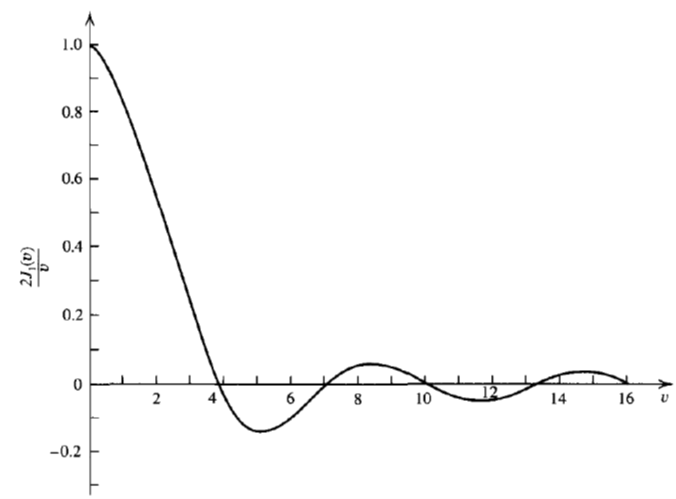
\includegraphics[width=\textwidth]{images/6_13_1.png}
  \end{minipage}%
  \hfill
  \begin{minipage}{0.4\textwidth}
    \centering
    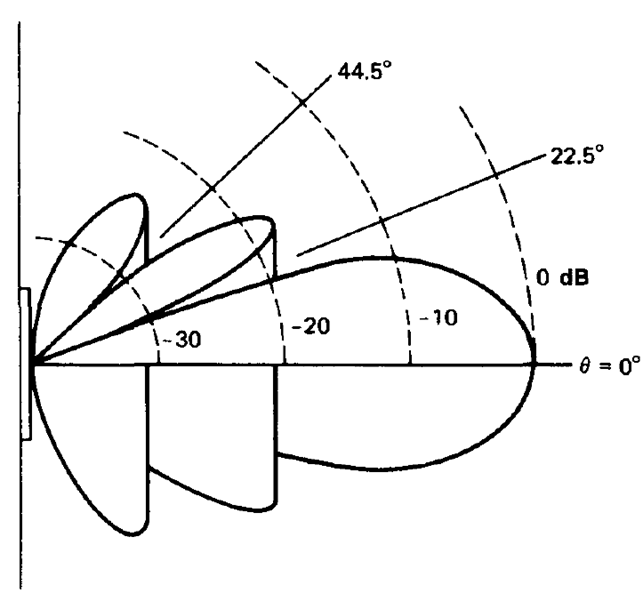
\includegraphics[width=\textwidth]{images/6_13_2.png}
  \end{minipage}
\end{figure}

This concludes our overview of sound sources, highlighting the key principles learned. The radiation behavior of a source is heavily dependent on its size. Small sources are inefficient radiators, but they are isotropic, radiating uniformly in all directions. In contrast, larger sources are more efficient radiators, but their radiation patterns are governed by interference, making them inherently non-isotropic. Small sources also exhibit a frequency-dependent behavior: for monopoles, radiated power scales with \(\omega^2\), while for dipoles, it scales with \(\omega^4\). For larger sources, interference effects dominate, and the radiation behavior depends on the ratio between the size of the source and the wavelength. This introduces a more complex frequency dependence, as the radiation pattern and efficiency change with variations in wavelength relative to the source size. This interplay underscores the importance of understanding both size and frequency in determining the radiation characteristics of sound sources.

\subsection{Reflection and Refraction}

The interaction between propagating waves becomes particularly significant when a wave encounters a boundary between two media with different properties. The key factor determining whether a medium is perceived as different by the wave is primarily the difference in propagation velocity. Such boundaries are at the core of refraction phenomena, where a wave changes direction as it crosses from one medium to another. Differences in absorption between the two media can also play a role.

When a plane wave hits an interface between two media, two main phenomena occur: reflection and refraction. The reflected wave remains in the original medium, maintaining its propagation velocity \( c \), while the refracted wave is transmitted into the second medium, where it travels at a different velocity \( c' \). 
 \begin{figure}[H]
    \centering
    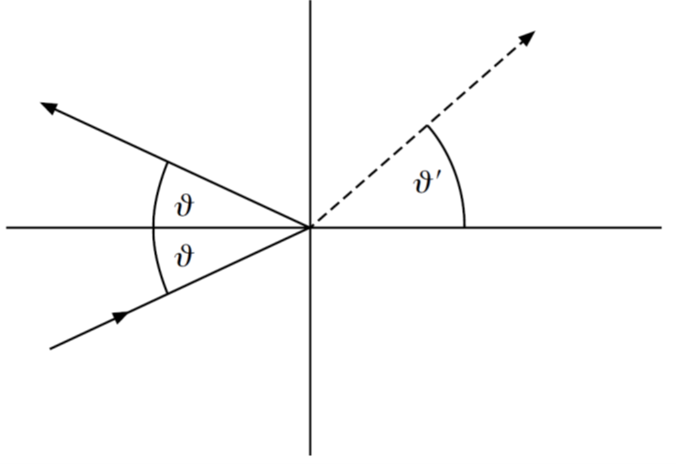
\includegraphics[width=0.45\textwidth]{images/6_14_1.png}
\end{figure}

The behavior of the waves at the boundary is governed by Snell's law, which is widely used in optics and acoustics. This law states that the reflection is specular, and the refracted wave propagates at a different angle. Mathematically, Snell's law is expressed as:

\[
n_1 \sin \theta_1 = n_2 \sin \theta_2 \quad \text{where} \quad n = \frac{c}{v}
\]

where \( n_1 \) and \( n_2 \) are the refractive indices of the two media, and \( \theta_1 \) and \( \theta_2 \) are the angles of incidence and refraction, respectively. To derive this law, we apply the continuity relations for acoustic variables—pressure and velocity—at the boundary. Specifically, the pressure must remain continuous across the boundary, and the normal component of the velocity must also be continuous. By applying these conditions, Snell's law emerges as a fundamental principle governing wave refraction:

\[
\frac{c}{\sin \theta} = \frac{c'}{\sin \theta'}
\]

Another way to approach this is through the principle of "trace fitting," which involves ensuring the continuity of the wavefronts at the interface. If the wave has a frequency \( f \) (determined by the oscillation of the source and independent of the medium), the wavelength will change depending on the propagation velocity of the medium. As the wave transitions from a medium with velocity \( c \) to one with \( c' \), the wavelength changes accordingly (\( \lambda \to \lambda' \)). 
 \begin{figure}[H]
    \centering
    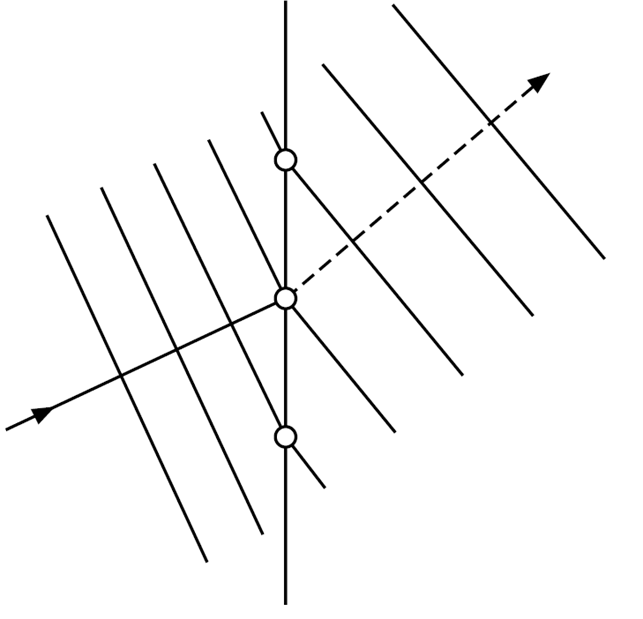
\includegraphics[width=0.4\textwidth]{images/6_14_2.png}
\end{figure}
The wavefront continuity condition ensures that the refracted wave follows the direction dictated by Snell's law. If \( c' > c \), so \( \lambda' > \lambda \), the refracted wave will deviate further from the normal, resulting in \( \theta' > \theta \). This analysis assumes plane waves hitting an infinite plane surface. However, when the interface is finite or when the wave has limited spatial extent, phenomena like scattering or diffusion must be considered.

A notable condition arises when \( \sin \theta' = \frac{c'}{c} \sin \theta \). If \( c' > c \), then \( \theta' > \theta \), and as \( \theta \) increases, \( \theta' \) eventually reaches \( 90^\circ \). Beyond this critical angle (angle of total reflection), for \( \theta_t > \arcsin(c / c') \), no transmitted wave propagates into the second medium. Instead, total internal reflection occurs, where all the wave energy is reflected back into the first medium.

Even in cases of total internal reflection, applying the continuity conditions for pressure and the normal component of velocity reveals the existence of an evanescent wave on the other side of the boundary. This wave does not propagate into the far field but instead decays exponentially with distance from the boundary. It represents a localized disturbance that remains confined to the vicinity of the boundary, without carrying energy away as a propagating wave.\\

To analyze how much of a wave is reflected and how much is refracted, we consider an incident plane wave with amplitude \(\hat{p}\), assuming harmonic behavior (\(e^{j\omega t}\)). The wave vector of the incident wave can be decomposed into its \(x\) and \(y\) components, capturing the direction of propagation relative to the boundary. 

\[
p_i(x, y, t) = p_i(x, y) e^{j \omega t} \quad \text{where} \quad p_i(x, y) = \hat{p} e^{-j k (x \cos \vartheta + y \sin \vartheta)}
\]

Upon reflection, the \(y\)-component of the wave vector remains unchanged, while the \(x\)-component reverses its sign, indicating the wave's propagation in the opposite direction along the \(x\)-axis. This symmetry arises due to the interaction with the boundary.
\[
p_r(x, y) = \hat{p} |R| e^{-j k (-x \cos \vartheta + y \sin \vartheta) + j \chi}
\]

Only a fraction of the wave is reflected, characterized by the reflection coefficient \(R\). This reflection factor may also introduce a phase shift due to the interaction with the boundary material, which can modify the reflected wave's phase. The reflection factor is expressed as a complex number:
\[
R = |R| e^{j\chi},
\]
where \(|R|\) denotes the magnitude of the reflection, and \(e^{j\chi}\) represents the possible phase shift.

The reflected wave is mathematically expressed as:
\[
p_r(x, y) = \hat{p} R e^{-j k (-x \cos \vartheta + y \sin \vartheta)},
\]





To analyze the reflection of a wave at a boundary, we consider the property of the wall, referred to as the wall impedance. The wall impedance, denoted as \( Z \), describes how the wall responds to a certain pressure with a given velocity and is defined as:
\[
Z = \left( \frac{p}{v_x} \right)_{x=0},
\]
where \( p \) is the pressure and \( v_x \) is the velocity normal to the wall.

We also introduce the specific wall impedance, denoted as \( \zeta \), which is the ratio of the wall impedance \( Z \) to the characteristic impedance of air \( Z_0 \):
\[
\zeta = \frac{Z}{Z_0}.
\]

For \( x < 0 \), which corresponds to the region to the left of the wall located at \( x = 0 \), the total pressure wave is the sum of the pressure of the incident wave and the reflected wave:
\[
p(x, y) = p_i + p_r = \hat{p} e^{-j k y \sin \vartheta} \left( e^{-j k x \cos \vartheta} + R e^{j k x \cos \vartheta} \right),
\]
where \( R \) is the complex reflection factor. Similarly, the velocity along the \( x \)-direction can be expressed as:
\[
v_x(x, y) = \frac{\hat{p}}{Z_0} e^{-j k y \sin \vartheta} \left( e^{-j k x \cos \vartheta} - R e^{j k x \cos \vartheta} \right) \cos \vartheta.
\]

Here, the term \( -R \) appears in the velocity equation because the impedance of the plane wave traveling backward (reflected wave) has an opposite sign compared to the forward (incident) wave. Additionally, the presence of \( \cos(\vartheta) \) arises because, when calculating the impedance, we consider the pressure acting on the wall and the transverse displacement of the wave along the \( x \)-direction. This ensures that the normal component of the velocity matches the boundary condition at the wall.

The reflection coefficient \( R \), which determines how much of the wave is reflected, is given by:
\[
R = \frac{Z \cos \vartheta - Z_0}{Z \cos \vartheta + Z_0} = \frac{\zeta \cos \vartheta - 1}{\zeta \cos \vartheta + 1}.
\]

The reflection phenomenon is closely tied to the discontinuity in impedance at the boundary. The discontinuity in the specific wall impedance leads to partial reflection and refraction of the wave. The wall impedance is generally a complex number, as it encompasses both propagation properties and absorption characteristics of the wall. A discontinuity in propagation velocity or absorption properties between two media manifests as a discontinuity in impedance, which subsequently governs the reflection and refraction phenomena at the boundary.

\subsection{Diffraction and Scattering}

In systems where we encounter an edge, we can describe the propagation of plane waves as a combination of numerous point sources emitting spherical waves. The envelope of all these spherical wavefronts explains why, when a wave encounters an edge or obstacle, the wavefront bends and propagates behind the obstacle. This phenomenon, known as diffraction, occurs due to the curvature of the edge wavefront. 

\begin{figure}[H]
    \centering
    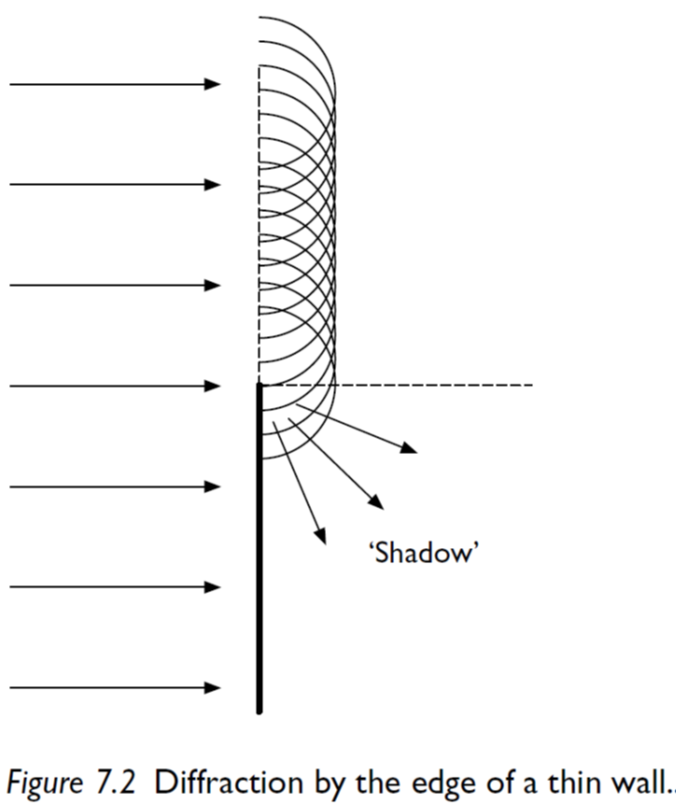
\includegraphics[width=0.4\textwidth]{images/6_17_2.png}
\end{figure}

The same principle applies not only to obstacles but also to finite objects. When a wave interacts with an object, it causes the object to oscillate, and this oscillation generates secondary waves. These secondary waves, radiated by the object set into motion, are part of a phenomenon referred to as scattering. Typically, we use the term \textbf{scattering} when waves are diffused by an object and \textbf{diffraction} when waves pass through apertures in obstacles. However, both phenomena arise from the same principle: the superposition of waves and interference effects.

If the object has dimensions comparable to or larger than the wavelength of the sound, it behaves like a simple curved surface. In such cases, the laws of specular reflection apply, and each sound wave reflects specularly relative to the surface's normal. This geometrical analysis considers only the direction of sound propagation, resulting in a shadowed area where the sound is weaker or absent and a region where the sound remains perceptible behind the object.

\begin{figure}[H]
    \centering
    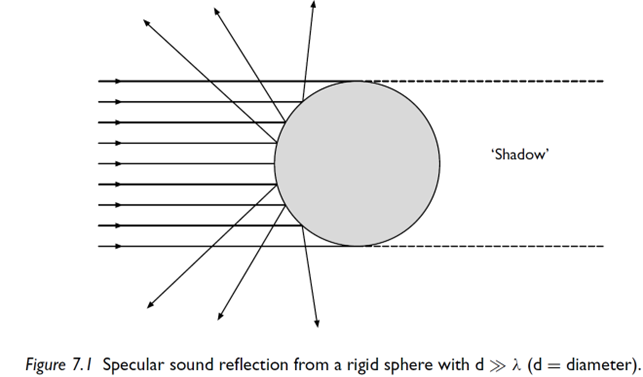
\includegraphics[width=0.65\textwidth]{images/6_17_1.png}
\end{figure}

As the size of the object decreases , the assumptions of ray-tracing analysis break down, and the wave nature of sound becomes dominant. In this scattering regime, the obstacle radiates a secondary sound field. The overall sound field then becomes a superposition of the primary field (the original wave) and the secondary, or scattered, radiation. Since this secondary radiation arises from the interference of all the vibrating elements of the object, it depends heavily on the geometry and size of the object.

When analyzing the diffraction by a rigid sphere, the polar pattern of scattered radiation changes depending on the sphere's size relative to the wavelength, represented here as \( ka \), where \( k \) is the wave number and \( a \) is the sphere's radius. The increase in the value of \( ka \) indicates that the sphere is becoming larger than the wavelength of the sound.. As shown in the figure, smaller spheres (e.g., \( ka = 1 \)) produce patterns that are nearly isotropic, with energy distributed almost uniformly in all directions. As the sphere size increases (e.g., \( ka = 3 \)), interference effects become more pronounced, creating distinct lobes in the polar pattern. For even larger spheres (e.g., \( ka = 5 \)), the interference results in sharper and more directional lobes.
\begin{figure}[H]
    \centering
    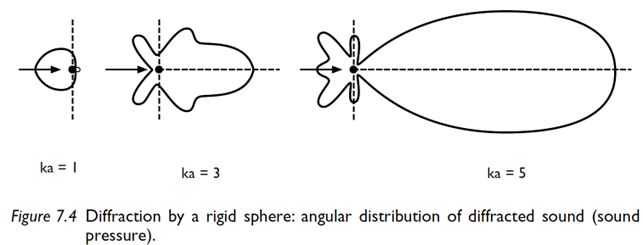
\includegraphics[width=0.75\textwidth]{images/6_18.png}
\end{figure}
The total acoustic field at any point is the sum of the plane wave incident on the sphere and the spherical wave scattered by the sphere. The scattering effect redistributes some of the energy from the forward direction into other directions. Unlike primary sources, which are externally driven, the radiation from extended objects like this sphere is secondary. The primary wave excites the sphere, setting it into motion and causing it to radiate energy with a characteristic pattern determined by the interference of the contributions from all points on the sphere's surface. This redistribution of energy away from the primary propagation direction into other directions is a key feature of scattering or diffusion phenomena.

To quantify the amount of energy scattered by an object when subjected to a primary plane wave, we use the concept of the scattering cross-section \( Q_s \). This parameter represents an effective area, expressing the power scattered by the object in all directions as if it were distributed over this effective area. The scattered power is proportional to the incident wave intensity \( I \), as given by \( P = A \cdot I \), where \( A \) is the effective area.

By directing a plane wave towards the object and measuring the power transmitted through it, the difference between the initial and transmitted power corresponds to the energy scattered into other directions. Dividing this scattered power by the original wave intensity allows us to calculate the effective scattering cross-section, which may differ from the object's geometric shadow.

\begin{figure}[H]
    \centering
    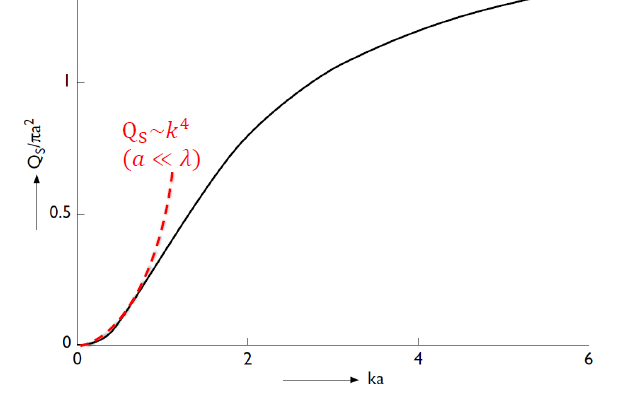
\includegraphics[width=0.6\textwidth]{images/6_19.png}
\end{figure}

The provided graph illustrates the scattering cross-section as a function of the size parameter \( ka \), where \( a \) is the radius of the sphere. For small objects (\( ka \ll 1 \)), the scattering cross-section increases with \( k^4 \), indicating that small spheres behave as dipoles, with efficiency scaling as \( k^4 \). As the sphere's size grows relative to the wavelength, the scattering becomes more complex, reflecting interference and geometry-dependent effects.\\


When discussing sound interaction with media, such as porous materials, we encounter phenomena where sound does not reach the other side of the medium. In fog, for instance, light is scattered away, reducing its ability to penetrate through the medium. Even if the energy is not absorbed but scattered in all directions, it produces a similar effect as absorption for an observer on the other side of the medium: the intensity is diminished or lost. This scattering can create a condition where the sound appears to be "absorbed," even though it is primarily being diffused.

From the perspective of sound transmission through a medium, both absorption and diffusion (scattering) lead to an apparent loss of intensity on the other side. In a porous material, sound is often trapped and bounced around inside the medium, which prolongs the sound's interaction time within the medium. This trapping increases the chances of energy dissipation due to absorption, making porous materials particularly effective at absorbing sound. Such materials are designed to trap sound waves for extended periods, ensuring greater absorption before the energy escapes the medium.

\begin{figure}[H]
  \centering
  \begin{minipage}{0.4\textwidth}
    \centering
    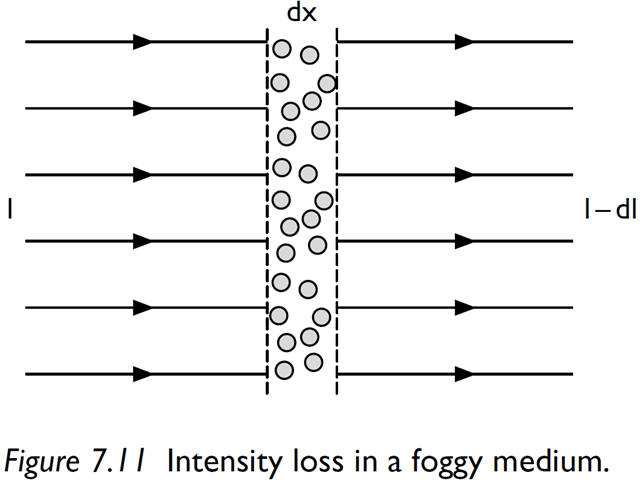
\includegraphics[width=\textwidth]{images/6_21_1.png}
  \end{minipage}%
  \hfill
  \begin{minipage}{0.4\textwidth}
    \centering
    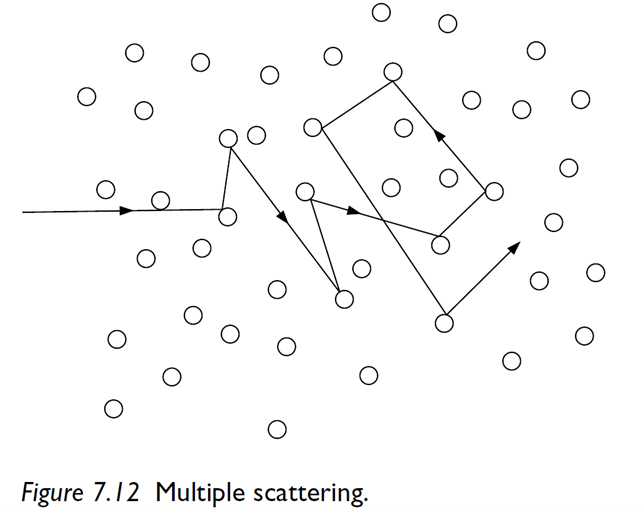
\includegraphics[width=\textwidth]{images/6_21_2.png}
  \end{minipage}
\end{figure}


In wave-particle interaction theory, extinction is defined as the sum of absorption and scattering. This means that, from a measurement perspective, it is often impossible to distinguish whether the sound's disappearance is due to high absorption by the material or extensive scattering. Both processes contribute to a lower intensity observed on the other side of the medium. From the observer's point of view, the sound "disappears" regardless of whether the dominant mechanism is absorption or scattering.\\


When analyzing the interaction between a sound wave and a complex object, such as a rough wall, we can identify three distinct regimes based on the relationship between the typical size of the roughness \( d \) and the wavelength \( \lambda \):

\begin{itemize}
    
\item Small Roughness Regime (\( d \ll \lambda \)):  
   In this regime, the roughness size \( d \) is much smaller than the wavelength \( \lambda \). From the perspective of the wave, the wall appears smooth and flat, and the incoming plane wave undergoes specular reflection. The surface behaves as if it were completely flat, with no significant scattering caused by the roughness.

\item Large Roughness Regime (\( d \gg \lambda \)):
   Here, the roughness size \( d \) is much larger than the wavelength \( \lambda \). Each section of the rough wall behaves like an independent flat surface, resulting in specular reflection at each part of the roughness. In this case, the wall can be considered as a collection of flat tiles, each reflecting the sound wave individually and specularly.
   

\item Intermediate Roughness Regime (\( d \sim \lambda \)): 
   When the roughness size \( d \) is comparable to the wavelength \( \lambda \), the wall behaves as a diffusing surface. In this regime, the interaction between the sound wave and the wall leads to significant scattering rather than specular reflection. This is the desired regime for designing diffusers, as the roughness causes the reflected sound energy to spread in multiple directions rather than concentrating in a single specular direction.
   
\end{itemize}

\begin{figure}[H]
    \centering
    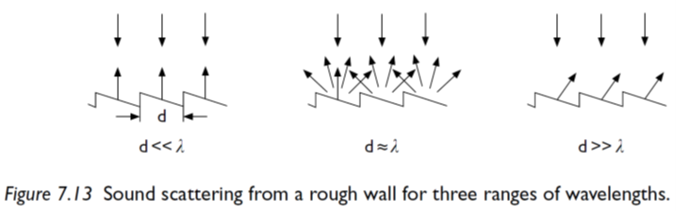
\includegraphics[width=0.65\textwidth]{images/6_22.png}
\end{figure}

\section{Pipes and horns. Turbulence in fluids}



We have studied mechanical vibrations in strings and membranes, as well as extended systems. Furthermore, we analyzed how individual sources radiate sound, specifically how vibrations translate into acoustic waves. This analysis was extended to continuous systems through surface or volume integration of infinitesimal sources. Additionally, we investigated the propagation of sound in uniform, isotropic environments, governed by the wave equation in a fluid. A natural next step is to consider what happens when a propagating wave encounters an obstacle. In this section, we will delve into the guiding of sound through structured paths, introducing the concept of sound waveguides.

\subsection{Pipes}

Pipes are essential components in musical instruments and acoustical systems, serving as resonators that guide and shape sound waves. A flute, for instance, functions as a simple resonator, essentially a truncated pipe. Beyond this, we can analyze more complex systems, such as pipes with junctions of varying cross-sections, and their effects on wave propagation. This leads to the broader concept of waveguides, including horns, which are designed to smooth the transition between a pipe and open air, reducing impedance mismatch and enhancing sound radiation. Additionally, we will explore the behavior of fluids within these systems, focusing on the physics of wave propagation in enclosed or semi-enclosed geometries.\\




We consider pipes as acoustic waveguides, where sound waves are confined and guided by the pipe itself. When studying sound wave propagation in pipes, two main assumptions are generally made:

\begin{itemize}
    \item  \textbf{Negligible frictional losses}. Since sound waves are longitudinal, the motion of air molecules in the acoustic wave is parallel to the walls of the pipe. Therefore, as a first approximation, the walls do not significantly affect wave propagation in tubes. Even for curved pipes, as long as the radius of curvature is much larger than the wavelength, the impact of the sidewalls can be considered negligible. Curved segments of pipes effectively guide sound from one point to another.

   However, in practice, wall boundaries introduce frictional losses due to local interactions between vibrating molecules and the walls. This results in sound attenuation, particularly near the wall regions where friction effects are prominent. The velocity profile of the fluid is uniform in the pipe, except for the boundary layer close to the walls, where friction causes a velocity gradient. These frictional effects cause an exponential loss in amplitude over the length of the pipe, leading to propagation losses due to absorption. For simplicity, we neglect these frictional losses in our analysis.
   
\begin{figure}[H]
    \centering
    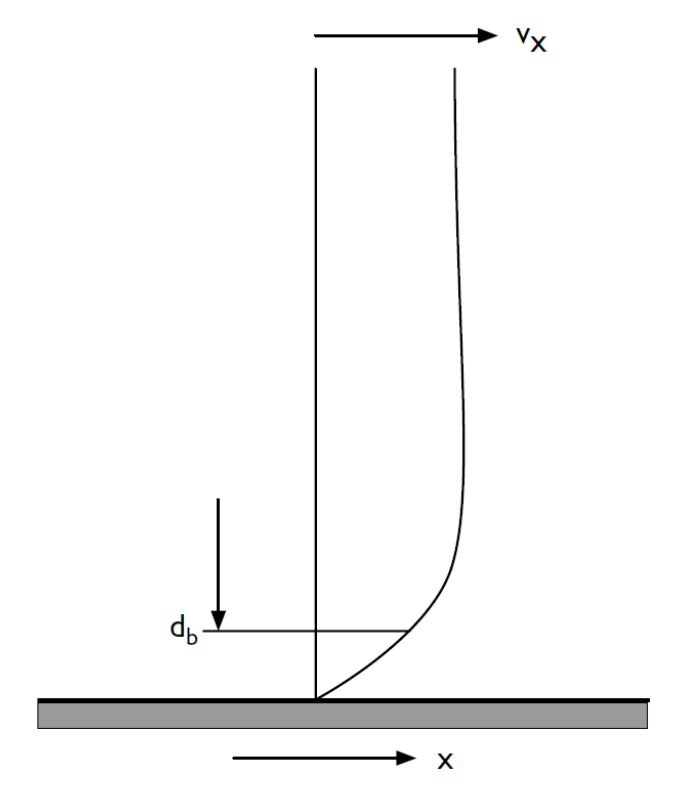
\includegraphics[width=0.4\textwidth]{images/7_3.png}
\end{figure}

\item \textbf{Plane wave propagation}
   A second approximation is that only plane waveforms propagate inside the pipe. This approximation holds true when the cross-section of the pipe is small compared to the wavelength of the sound. However, as the cross-section increases, the pipe can support higher-order modes of propagation. These modes are characterized by non-uniform phase profiles in the transverse plane of the pipe. 
\end{itemize}


\subsection{Infinite Transmission Line}

In this section, we consider an infinite transmission line or waveguide. The goal is to determine the values of pressure \( p(x) \) and velocity \( v(x) \) at a specific position \( x \), given their known values at a reference position \( x = 0 \). This approach allows us to express the pressure and velocity wave propagating along the waveguide in terms of their values at one specific position.

\begin{figure}[H]
    \centering
    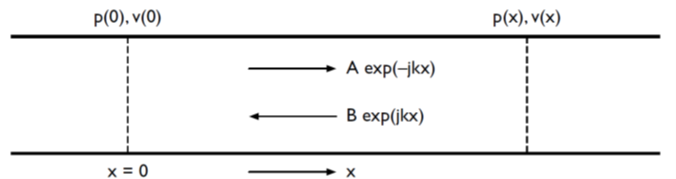
\includegraphics[width=0.7\textwidth]{images/7_4.png}
\end{figure}

We assume the plane wave solutions for the propagation (because of the small cross-section of the transmission line):
\[
p(x) = A e^{-jkx} + B e^{jkx}, \quad Z_0 v(x) = A e^{-jkx} - B e^{jkx}.
\]

These represent two solutions, where one propagates to the right and the other to the left. Here, \( A \) and \( B \) are the wave amplitudes, \( k \) is the wavenumber, and \( Z_0 \) is the characteristic impedance. The impedance of the forward-propagating wave is \( Z_0 \), and for the backward-propagating wave, it is \( -Z_0 \).

Using trigonometric identities, we can rewrite the pressure and velocity expressions in terms of sine and cosine:
\[
p(x) = (A + B) \cos(kx) - j (A - B) \sin(kx),
\]
\[
Z_0 v(x) = (A - B) \cos(kx) - j (A + B) \sin(kx).
\]



To determine the specific values of \( A \) and \( B \), we apply the boundary conditions. At \( x = 0 \), the values of pressure \( p(0) \) and velocity \( v(0) \) are known:
\[
p(0) = A + B, \quad Z_0 v(0) = A - B.
\]

From these boundary conditions, \( A \) and \( B \) can be expressed as:
\[
A = \frac{p(0) + Z_0 v(0)}{2}, \quad B = \frac{p(0) - Z_0 v(0)}{2}.
\]



Using the values of \( A \) and \( B \) derived above, the pressure \( p(x) \) and velocity \( v(x) \) at any position \( x \) can be expressed as:
\[
p(x) = p(0) \cos(kx) - j Z_0 v(0) \sin(kx),
\]
\[
Z_0 v(x) = -j p(0) \sin(kx) + Z_0 v(0) \cos(kx).
\]

These expressions provide the pressure and velocity waveforms at any position \( x \) along the waveguide, given their known values at \( x = 0 \). 



It is important to note that this analysis does not necessarily assume the system is a transmission line or waveguide. It is valid for any plane wave propagating in a harmonic regime. Here, the analysis is depicted assuming the solution exists only within the walls of the pipe and not outside it, but the general method applies to any harmonic solution.

\subsection{Finite Transmission Line}



When studying waveguides, it is often necessary to analyze the behavior of a pipe that is truncated at one end. This truncation can take various forms, such as an open pipe, a closed pipe, a horn, or a membrane. Generally, the truncation is modeled as a load impedance \( Z_L \). If the truncation has a specific impedance \( Z_L \), we want to understand the input impedance \( Z_\text{IN} \) measured at the entrance of the waveguide segment of length \( l \). This segment terminates with the load impedance \( Z_L \).
\begin{figure}[H]
    \centering
    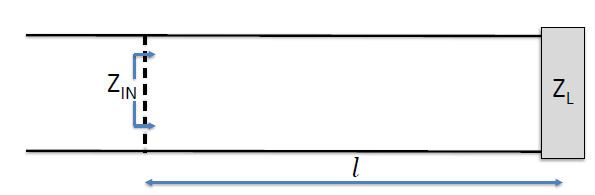
\includegraphics[width=0.6\textwidth]{images/7_5.png}
\end{figure}
Starting from the general expressions of pressure \( p(x) \) and velocity \( v(x) \), we evaluate the input impedance at \( x = -l \) based on the load impedance at \( x = 0 \). The input impedance \( Z_\text{IN} \) is defined as:



\[
Z_\text{IN} = \frac{p(-l)}{v(-l)}.
\]

Using the expressions for \( p(x) \) and \( v(x) \):

\[
p(x) = p(0) \cos(kx) - j Z_0 v(0) \sin(kx),
\]
\[
Z_0 v(x) = -j p(0) \sin(kx) + Z_0 v(0) \cos(kx),
\]

we substitute \( x = -l \) to compute \( p(-l) \) and \( v(-l) \). Simplifying the trigonometric terms and substituting \( Z_L = \frac{p(0)}{v(0)} \), the input impedance becomes:

\[
Z_\text{IN} = Z_0 \frac{Z_L + j Z_0 \tan(kl)}{Z_0 + j Z_L \tan(kl)}.
\]


This relationship shows that the input impedance depends strongly on the length \( l \) of the pipe segment and the frequency of the wave, as \( k = \frac{2\pi}{\lambda} \). Consequently, the same pipe can exhibit different impedance behavior for different frequencies.


\begin{itemize}
    \item  \textbf{Quarter-Wavelength Behavior} (\( kl = \frac{\pi}{2} + m\pi \)):

   When \( kl = \frac{\pi}{2} + m\pi \), the tangent term diverges, simplifying the impedance expression to:

   \[
   Z_\text{IN} = \frac{Z_0^2}{Z_L}.
   \]

   This behavior indicates that for a quarter-wavelength pipe, the input impedance becomes inversely proportional to the load impedance. For example, a large load impedance \( Z_L \) is perceived as a small input impedance at the entrance of the pipe.

\item \textbf{Rigid End Plate} (\( Z_L \to \infty \)):

   When the pipe is closed at the end (\( Z_L \to \infty \)), the input impedance becomes:

   \[
   Z_\text{IN} = -j Z_0 \cot(kl).
   \]

 Resonances occur when \( \cot(kl) = 0 \), corresponding to specific lengths where standing waves are formed. This means the resonant frequencies depend on the pipe's length, allowing you to tune the pipe's length to achieve resonance for any specific boundary condition or load impedance.

\end{itemize}

In essence, this behavior is similar to the normal modes in a string. When a string is fixed at both ends, it supports resonances at specific lengths that correspond to half a wavelength, a full wavelength, and so on. These resonances arise due to the boundary conditions of the system, which dictate the allowed modes of vibration. Similarly, in a pipe, by tuning the load impedance at the ends, we effectively modify the boundary conditions, enabling resonance under different conditions depending on the specific load impedance.

If we consider a plane wave within a pipe with two walls acting as the load impedance, infinite rigid walls imply that the velocity at the walls is zero. This leads to the formation of standing waves where the velocity nodes coincide with the wall positions. For instance, in the first mode (the fundamental), the velocity is zero at the ends, and the pressure forms a standing wave pattern. This standing wave is the result of waves bouncing back and forth within the pipe, combining through constructive interference. As the wave completes its round trip, its phase accumulates, and constructive interference occurs, reinforcing the standing wave.

Changing the load impedance, which is a complex number, alters the material properties of the walls. This change affects the reflection coefficient's phase, meaning that each time the sound wave reflects off the wall, it accumulates an additional phase shift. This phase shift is not directly related to the wavelength but instead depends on the mechanical response of the wall (the load). Intuitively, this additional phase contribution is equivalent to modifying the room's effective length, making it slightly longer or shorter than with perfectly rigid walls. By adjusting the load impedance and thereby the phase accumulated during reflections, we change the effective length of the pipe and the corresponding resonant frequencies.

Once the load impedance is determined, it can be plugged into the expression for the input impedance to predict the resonant conditions. This is the principle underlying the tuning of organ pipes, where resonance is adjusted by modifying the effective boundary conditions at the pipe's ends.

\subsection{Pipes Discontinuities}


Previously, cross-sections played no role, but here we introduce a discontinuity due to the difference in cross-sectional areas of two connected pipes. We know that narrower or wider sections of a pipe represent different propagation media for the guided mode. This means that when a sound wave encounters such a boundary, part of it is reflected back, while the rest is transmitted forward.
\begin{figure}[H]
    \centering
    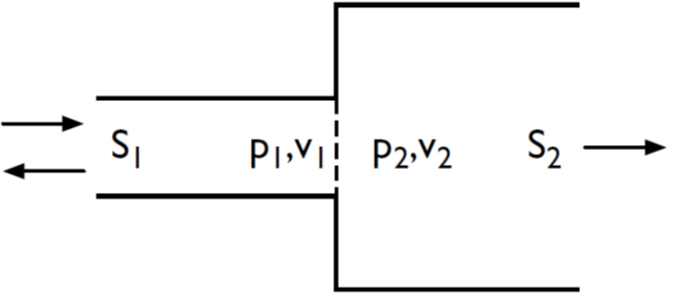
\includegraphics[width=0.5\textwidth]{images/7_6.png}
\end{figure}
Assuming an incident wave \( p_i \), we represent the total pressure to the left (\( p_1 \)) as the sum of the incident wave and the reflected wave, while the total pressure to the right (\( p_2 \)) corresponds only to the transmitted wave:

\[
p_1 = p_i (1 + R), \quad p_2 = T p_i.
\]

Here, \( R \) and \( T \) are the reflection and transmission coefficients, respectively. At the boundary between two sections, the pressure must remain continuous(conservation of energy); otherwise, it would create infinite forces, which is physically impossible. Thus, we impose the condition:

\[
p_1 = p_2 \quad \Rightarrow \quad 1 + R = T.
\]

In contrast, the velocity is not continuous at the boundary. By considering the conservation of mass flow rate (analogous to a fluid flow), we have:

\[
v_1 S_1 = v_2 S_2,
\]

where \( S_1 \) and \( S_2 \) are the cross-sectional areas of the left and right sections, respectively. This implies that as the cross-sectional area changes, the velocity must also adjust to conserve the total flow. 

Using the acoustic impedance \( Z_0 = \frac{p}{v} \), we express the velocities \( v_1 \) and \( v_2 \) in terms of the pressures:

\[
v_1 = \frac{p_i}{Z_0} - \frac{R p_i}{Z_0}, \quad v_2 = \frac{T p_i}{Z_0}.
\]

Substituting these into the continuity equation for the mass flow:

\[
S_1 (1 - R) \frac{p_i}{Z_0} = S_2 T \frac{p_i}{Z_0}.
\]

From these conditions, we solve for the reflection (\( R \)) and transmission (\( T \)) coefficients as functions of the cross-sectional areas:

\[
R = \frac{S_1 - S_2}{S_1 + S_2}, \quad T = \frac{2 S_1}{S_1 + S_2}.
\]

When there is no discontinuity (\( S_1 = S_2 \)), both \( R \) and \( T \) vanish or become 1, respectively, and no reflection occurs. However, as soon as the cross-sections differ (\( S_1 \neq S_2 \)), a reflection coefficient arises. 


Considering the strings, we expressed the reflection and transmission coefficients in terms of the impedances of the media. Here, we reformulate them based on the cross-sectional areas of the pipes. The relationship between the impedance discontinuity and the cross-sectional discontinuity is directly proportional: the ratio of the impedances matches the ratio of the cross-sectional areas.

From the boundary conditions, we know:

\[
\begin{cases}
p_1 = p_2, \\
v_1 S_1 = v_2 S_2,
\end{cases}
\]


Using the definition of impedance \( Z = \frac{p}{v} \), we write:

\[
\frac{p_1}{v_1} = \frac{p_2}{v_2} \frac{S_1}{S_2}.
\]

This implies:

\[
\frac{Z_1}{Z_2} = \frac{S_1}{S_2},
\]

where \( Z_1 \) and \( Z_2 \) are the acoustic impedances of the two sections. This result shows that the impedance discontinuity is governed entirely by the ratio of the cross-sectional areas of the two sections.\\

This setup can create a resonant cavity:
\begin{figure}[H]
    \centering
    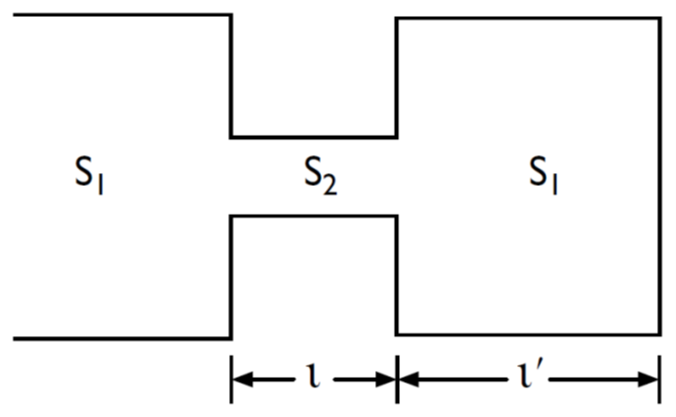
\includegraphics[width=0.4\textwidth]{images/7_6_1.png}
\end{figure}
If there are reflections at both cross-sectional boundaries, sound waves bounce back and forth within the central section (S2 in the image below). Certain frequencies may resonate, building up over time. Unlike perfect reflections (as with rigid walls), the reflections here are partial, meaning some energy is lost at each reflection. Despite these losses, partial reflections can still lead to resonances caused by the discontinuity in the pipe’s geometry.

\subsection{Resonators}


Let's consider a schematic representation of a Helmholtz resonator. It consists of a narrow channel situated between two wider environments. A guided sound wave propagates from the left through an infinite waveguide, encounters the narrow channel, and terminates in a wider section with a perfectly rigid wall at its end. The parameters defining the system are the cross-sectional areas $S_1$ and $S_2$ of the wider regions and the narrow channel, respectively, and the lengths $l$ and $l'$ of the narrow channel and the final wide section.

The objective is to analyze the acoustic response of this system, particularly to compute the input impedance measured at the entrance of the resonator. This impedance characterizes how the guided sound wave interacts with the resonator, acting as a measure of its acoustic behavior.

To perform the analysis, we start from the rigid wall at the end of the system and work backward through the resonator. At the rigid wall, the impedance is infinite, and the load impedance at this point is viewed through the length $l'$ of the final section. Moving back through the junction between $S_2$ and $S_1$, the impedance experiences a discontinuity due to the change in cross-sectional area. Further backward, the impedance is evaluated along the narrow channel of length $l$. At the left-side junction, another discontinuity occurs, as the impedance transitions from $S_2$ to $S_1$. By considering these sequential steps, the total impedance of the resonator can be determined, taking into account all geometric and boundary conditions.

\begin{figure}[H]
    \centering
    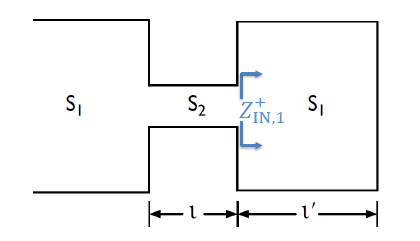
\includegraphics[width=0.4\textwidth]{images/7_8_1.png}
\end{figure}
At the rigid wall, the input impedance of the final section, as seen through the length $l'$, is given by:
\[
Z_\text{IN,1}^+ = -j Z_0 \cot(k l'),
\]
where $Z_0$ is the characteristic impedance of the system, and $k$ is the wavenumber. Assuming that the system dimensions are much smaller than the wavelength, such that $k l' \ll 1$, this expression simplifies to:
\[
Z_\text{IN,1}^+ \approx -\frac{j Z_0}{k l'} = -\frac{j \rho_0 c}{k l'} = \frac{\rho_0 c^2}{j \omega l'},
\]
where $\rho_0$ is the density of the medium, $c$ is the speed of sound, and $\omega$ is the angular frequency. We observe a resonant behavior, known as Helmholtz resonance, which differs significantly from the previously discussed constructive interference-based resonance, as it can occur even for lengths much smaller than the wavelength, unlike the latter.

\begin{figure}[H]
    \centering
    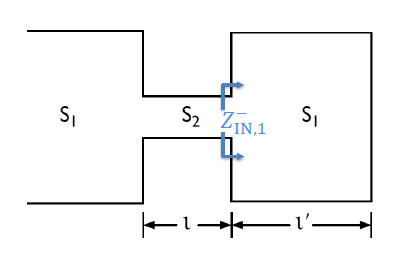
\includegraphics[width=0.4\textwidth]{images/7_8_2.png}
\end{figure}
When moving backward across the junction between the narrow channel with cross-sectional area $S_2$ and the wider section with cross-sectional area $S_1$, the impedance changes due to the cross-sectional ratio. This discontinuity results in the relation:
\[
Z_\text{IN,1}^- = Z_\text{IN,1}^+ \frac{S_2}{S_1}.
\]

The impedance discontinuity at this junction leads to a smaller impedance, corresponding to a higher velocity in the narrower section. 


 \begin{figure}[H]
    \centering
    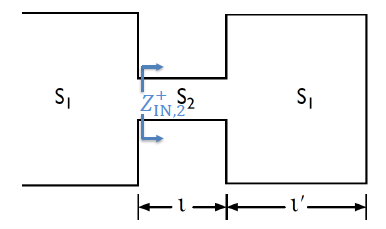
\includegraphics[width=0.4\textwidth]{images/7_9_1.png}
\end{figure}
 We now step backward along the length \( l \), computing the input impedance at the second chamber (\( Z_{\text{IN},2}^+ \)), located just to the right of the second junction.
 \[Z_{\text{IN},2}^+ = Z_0 \frac{Z_{\text{IN},1}^- + j Z_0 \tan(kl)}{Z_0 + j Z_{\text{IN},1}^- \tan(kl)}
\]
 Using the same approximation as before, where \( kl \ll 1 \), we simplify the expression for the input impedance:

\[
Z_{\text{IN},2}^+ \approx Z_0 \frac{Z_{\text{IN},1}^- + j Z_0 k l}{Z_0 + j Z_{\text{IN},1}^- k l}.
\]


\begin{figure}[H]
    \centering
    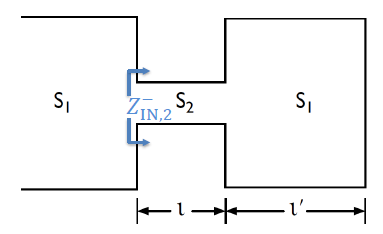
\includegraphics[width=0.4\textwidth]{images/7_9_2.png}
\end{figure}
Next, crossing the second junction at \( S_2 \) and stepping back to the larger section \( S_1 \), the minus-side impedance (\( Z_{\text{IN},2}^- \)) is calculated as the right-side impedance (\( Z_{\text{IN},2}^+ \)) scaled by the ratio of the cross-sections:

\[
Z_{\text{IN},2}^- = Z_{\text{IN},2}^+ \frac{S_1}{S_2} = j \rho_0 c \frac{S_1} {S_2} \frac{\frac{\omega l}{c} S_1 - \frac{c}{\omega l'} S_2}{S_1 + \frac{l}{l'} S_2}
\]

The resonant frequency of the Helmholtz resonator can be identified by setting the numerator of the impedance equal to zero, as resonance corresponds to the condition where pressure is minimal, and velocity is maximal. Solving for \( \omega \), we derive the resonance frequency as:

\[
\omega_{\text{RES}} = \sqrt{\frac{c^2 S_2}{l' l S_1}}.
\]

we observe that the denominator contains the volume of the chamber on the right, \( V = l' S_1 \). This shows that the resonance frequency depends on the volume of the main chamber. The numerator involves the cross-sectional area \( S_2 \) of the tube, while the denominator also includes the tube's length \( l \). Many musical instruments operate based on this principle, such as the ocarina or the guitar. 

For example, in the guitar, the Helmholtz resonance plays a significant role alongside other mechanical resonances. Most of the resonances in a guitar are mechanical, originating from the wooden parts of the instrument. However, there is also an acoustic Helmholtz resonance, determined by the hole in the guitar's body, which enhances specific frequencies. Similarly, the resonance in an empty bottle functions as a sharp resonator, producing a distinct frequency.

\begin{figure}[H]
  \centering
  \begin{minipage}{0.35\textwidth}
    \centering
    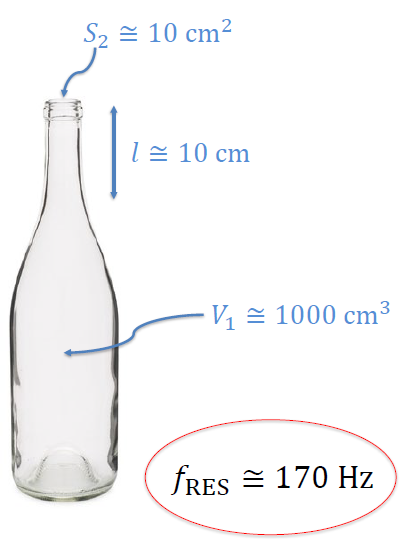
\includegraphics[width=\textwidth]{images/7_10.png}
  \end{minipage}%
  \hfill
  \begin{minipage}{0.4\textwidth}
    \centering
    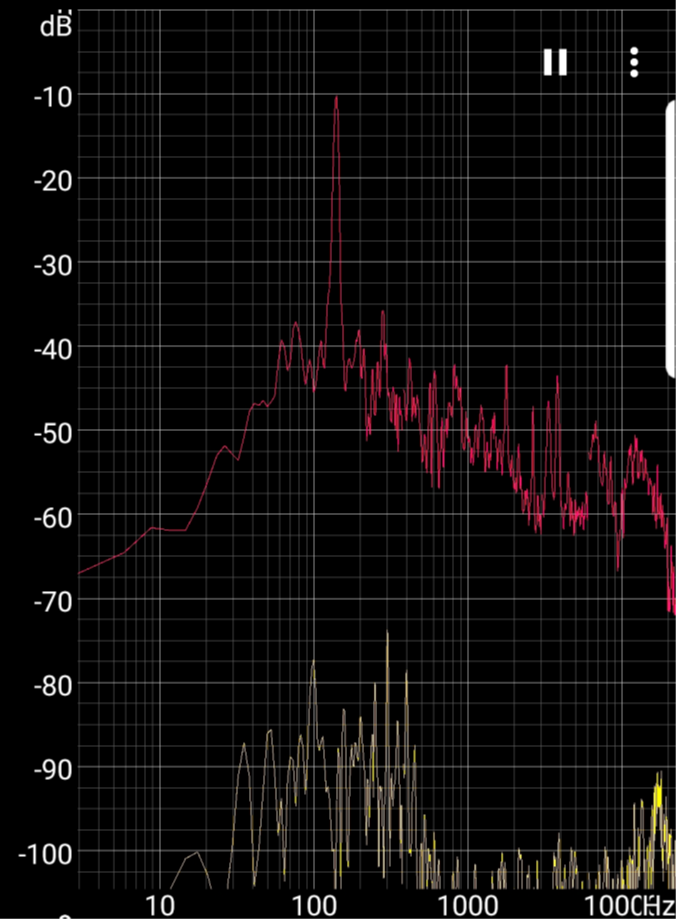
\includegraphics[width=\textwidth]{images/7_11.png}
  \end{minipage}
\end{figure}


A Helmholtz resonator can, in principle, sustain other resonances as well. If we consider the input impedance of the main chamber, which is proportional to \( \frac{1}{k l'} \), additional resonances can arise due to sound bouncing back and forth inside the end chamber \( S_1 \). These resonances are standing waves formed by the propagation of sound within the chamber. However, these resonances disappear when the chamber's length \( l' \) becomes much smaller than the wavelength of the sound.

Thus, the system exhibits two different regimes: the Helmholtz resonance and the standing wave resonances. These depend on the geometry and input impedance of the system. The standing wave resonances, also known as Fabry-Pérot resonances, occur when waves bounce back and forth, creating standing waves. These resonances are based on the accumulation of phase during propagation and depend on the cavity's length. Fabry-Pérot resonators arise due to reflections at both boundaries, producing constructive interference for specific frequencies.

In addition to Helmholtz and Fabry-Pérot resonances, acoustic systems often exhibit mechanical resonances. These are influenced by the material properties, geometry, and boundary conditions of the system. Mechanical resonances significantly affect the acoustic response of an instrument, modifying the behavior of acoustic waves.

For musical instruments, Fabry-Pérot standing wave resonances are generally negligible due to the small size of the instrument relative to the wavelength of sound. Instead, the Helmholtz resonance and mechanical resonances dominate the acoustic response, shaping the instrument's sound characteristics.

\subsection{Large Cross Section}



When analyzing wave propagation within confined boundaries, we consider specific approximations. One approximation assumes minimal friction, while the second assumes that the cross-section of the waveguide is sufficiently small to support only plane wave guided modes. However, when the cross-section becomes larger, the waveguide begins to support higher-order modes, much like the behavior observed in vibrating membranes.

\begin{figure}[H]
    \centering
    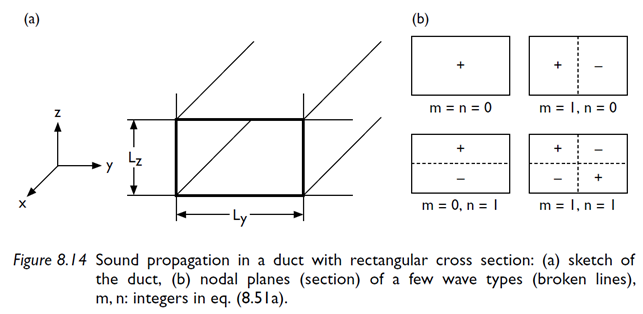
\includegraphics[width=0.7\textwidth]{images/7_12.png}
\end{figure}

For a rectangular waveguide with transverse cross-sectional dimensions \( L_z \) and \( L_y \), solving the wave equation reveals that the smallest cross-section supports the fundamental guided mode (\( m = n = 0 \)). This fundamental mode exhibits no nodal lines in the cross-section, and its phase remains uniform across the section, resembling a plane wave propagating through the pipe.

As the dimensions of the cross-section increase, higher-order modes emerge. For instance, the \( m = 1 \) mode introduces a vertical nodal line, while the \( n = 1 \) mode introduces horizontal nodal lines. Additionally, the \( + \) and \( - \) signs in these modes indicate a 180-degree phase shift between specific regions of the cross-section, dictated by the boundary conditions imposed by the waveguide.



The emergence of higher-order modes within waveguides leads to several significant phenomena:
\begin{itemize}
    \item  \textbf{Existence of Higher-Order Modes:} These modes are not plane waves, and their behavior differs significantly from that of fundamental modes.
\item \textbf{Cutoff Frequency:} Each higher-order mode has a cutoff frequency \( \omega_m \) , below which it cannot propagate. This means that higher-order modes only exist for frequencies sufficiently high (or wavelengths sufficiently short) relative to the dimensions of the waveguide's cross-section \( \omega >\omega_m \) . At low frequencies or long wavelengths, only the fundamental mode is supported.
\item \textbf{Dispersion:} Higher-order modes propagate at different speeds compared to plane waves in an isotropic medium. Only the fundamental mode propagates at the same speed as in air. The propagation speed of each mode must be considered when calculating the wave vector \( k \). This phenomenon is analogous to light propagation in optical waveguides, where the mode index quantifies the reduction in propagation speed for each mode.

The dispersion relation for higher-order modes is given by:

\[
c' = \frac{c}{\sqrt{1 - \left(\frac{\omega_m}{\omega}\right)^2}},
\]

where \( \omega_m \) is the cutoff frequency of the mode and \( c' \) is the mode's propagation speed.
\end{itemize}


For square and rectangular waveguides, the solutions to the wave equation are relatively straightforward. For circular waveguides, the analysis becomes more complex, involving two indices: one indicating the number of tangential nodal lines and the other indicating the number of radial nodal lines. These indices combine to define the mode structure. However, as long as the cross-section of the waveguide remains much smaller than the wavelength, higher-order effects are negligible, and the fundamental mode dominates.

\subsection{Horns}



When dealing with wave propagation in pipes, it is important to consider the behavior at the boundaries. If the pipe ends with an infinite rigid wall, there is 100\% reflection of the sound wave due to the impedance discontinuity. Surprisingly, even in the case of an open end, there is also 100\% reflection. This occurs because moving from a finite cross-section (the pipe) to an effectively infinite cross-section (the open air) creates a significant impedance mismatch, leading to a similar reflection phenomenon. Although both closed and open ends result in full reflection, they impose different boundary conditions. For a closed end, the velocity at the boundary must be zero, while for an open end, the pressure must equal the ambient pressure.

Inside a pipe, sound waves reflect back and forth, creating resonances. In an idealized scenario, the sound remains confined within the pipe and does not escape. However, in practice, the edges of the pipe at the open end act as scattering objects. These edges scatter some of the modes of the plane waves propagating within the pipe, causing a portion of the sound to radiate out into the surrounding space.


To improve the ability of the sound waves to transition from the pipe to open space, it is necessary to reduce the impedance discontinuity between the pipe and the open air. One effective method is to gradually widen the cross-section at the end of the pipe, creating a smooth transition between the confined space of the pipe and the open air. This technique, known as \emph{impedance matching}, minimizes reflection and enhances sound radiation efficiency. Musical instruments often incorporate this principle by utilizing horns at their open ends. 

To analytically describe how sound waves propagate in waveguides with changing cross-sections, we start by recalling the principles used for standard plane waves: the force balance and the mass balance. 


\[ \text{Force balance:} \quad
-\frac{\partial p}{\partial x} = \rho_\text{TOT} \left( \frac{\partial v_x}{\partial t} + v_x \frac{\partial v_x}{\partial x} \right),
\]


\[\text{Mass balance:} \quad
-v_x \frac{\partial \rho_\text{TOT}}{\partial x} - \rho_\text{TOT} \frac{\partial v_x}{\partial x} = \frac{\partial \rho}{\partial t}.
\]


We adapt these principles to the new geometry, where the waveguide cross-section varies along the propagation direction. 

We consider a small volume of the waveguide bounded between two cross-sections at positions \(x\) and \(x + \mathrm{d}x\). The cross-sectional area at any position \(x\) is described by a function \(S(x)\), which specifies how the waveguide's surface changes along the propagation direction.
\begin{figure}[H]
    \centering
    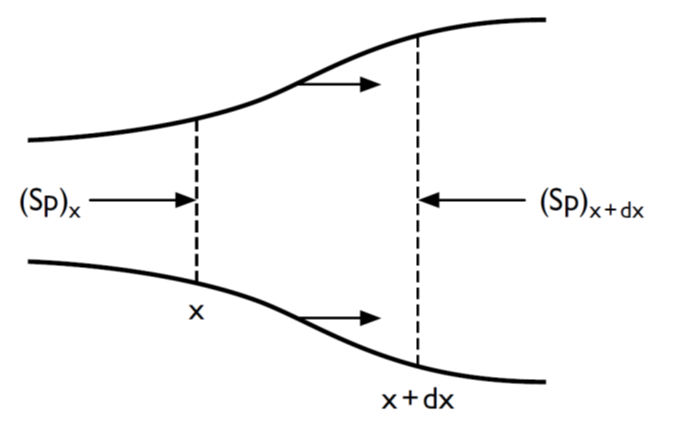
\includegraphics[width=0.5\textwidth]{images/7_16.png}
\end{figure}

The forces acting on the volume element include: the pressure force acting on the left boundary, \(p(x) S(x)\), the pressure force acting on the right boundary, \(-p(x + \mathrm{d}x) S(x + \mathrm{d}x)\), a reaction force due to the inclined walls created by the changing cross-section.

By Taylor expanding the pressure and cross-sectional area about \(x\), we derive the force balance equation:

\[
(Sp)_x - (Sp)_{x+dx} + [S(x+dx) - S(x)]p(x) = \rho_0 \frac{\partial v_x}{\partial t} S dx \quad \implies \quad -S \frac{\partial p}{\partial x} = \rho_0 \frac{\partial (S v_x)}{\partial t},
\]

where \(\rho_0\) is the equilibrium density, \(v_x\) is the particle velocity in the \(x\)-direction, and \(S\) is the cross-sectional area.


The mass balance is similarly derived, considering the flow of mass through the boundaries of the volume. After Taylor expanding the terms and considering that \(S\) is a function of \(x\) (so it goes inside the expansion), we arrive at the equation:

\[ (\rho_t v_x S)_{x+dx} - (\rho_t v_x S)_x = - S dx \frac{\partial \rho}{\partial t} \quad \implies \quad
\rho_0 \frac{\partial (S v_x)}{\partial x} = -\frac{S}{c^2} \frac{\partial p}{\partial t},
\]

where \(c\) is the speed of sound. By differentiating the force balance equation with respect to \( x \) and the mass balance equation with respect to \( t \), and then combining the two, we eliminate the velocity \( v_x \) to derive an equation entirely in terms of the pressure \( p \). The result is Webster's equation, which describes sound wave propagation in a waveguide with variable cross-section:

\[
\frac{1}{S} \frac{\partial}{\partial x} \left( S \frac{\partial p}{\partial x} \right) = \frac{1}{c^2} \frac{\partial^2 p}{\partial t^2}.
\]

This equation can also be written in an alternative form:

\[
\frac{\partial^2 p}{\partial x^2} + \frac{\mathrm{d} (\ln S)}{\mathrm{d} x} \frac{\partial p}{\partial x} = \frac{1}{c^2} \frac{\partial^2 p}{\partial t^2}.
\]


When \(S(x)\) is constant, \(\mathrm{d}(\ln S)/\mathrm{d}x = 0\), and Webster's equation reduces to the standard wave equation for plane waves:

\[
\frac{\partial^2 p}{\partial x^2} = \frac{1}{c^2} \frac{\partial^2 p}{\partial t^2}.
\]

This demonstrates that Webster's equation generalizes the wave equation to account for the effects of varying cross-sectional area, enabling the description of wave propagation in horns and other non-uniform waveguides.

\begin{figure}[H]
    \centering
    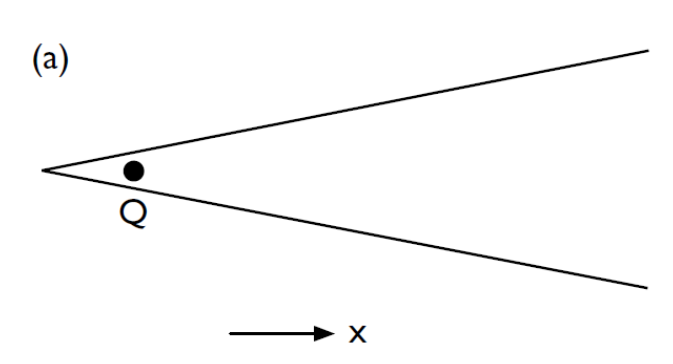
\includegraphics[width=0.4\textwidth]{images/7_17.png}
\end{figure}

To solve Webster's equation for a horn, we need to know the shape of the horn, represented by \( S(x) \). In the case of a conical horn, the cross-sectional area increases as \( S(x) = A x^2 \). Substituting this expression into Webster's equation yields:

\[
\frac{\partial^2 p}{\partial x^2} + \frac{2}{x} \frac{\partial p}{\partial x} = \frac{1}{c^2} \frac{\partial^2 p}{\partial t^2}.
\]

This is identical to the wave equation in spherical coordinates for radial waves. However, here the wave propagates only along the \( x \)-axis, as it is confined by the conical horn. The solution to this equation can be interpreted as a spherical wave confined to the horn, propagating in the \( x \)-direction. 

The pressure distribution for a spherical wave in free space is given by:

\[
p(r, t) = \frac{j \omega \rho_0 \hat{Q}}{4 \pi r} e^{j(\omega t - kr)}.
\]

For a conical horn, the pressure distribution along the \( x \)-axis is expressed as:

\[
p(x, t) = \frac{j \omega \rho_0 \hat{Q}}{\Omega x} e^{j(\omega t - kx)},
\]

where \( \Omega \) represents the solid angle of the horn. The conical horn channels the spherical wave radiated by the source at the entrance (modelled as a point source), focusing it within the solid angle \( \Omega \). This confinement leads to an increase in intensity by a factor of \( \frac{4\pi}{\Omega} \) for pressure and \( \frac{4\pi}{\Omega^2} \) for intensity, as compared to free-space propagation. 

The intensity of the wave decays as \( 1/x^2 \), similar to a spherical wave in free space, but is now channeled within the horn. Additionally, the horn reduces reflections at the open end by gradually transitioning the impedance from the horn to free space, further improving the efficiency of sound propagation.

\subsection{Dynamics of Air Jets}


Flutes and pipes share a similar mechanism of sound production, where an air jet, either produced by the mouth of the player or the pump of an organ, strikes a sharp object (such as the edge of a flute embouchure hole). This interaction leads to two key effects: (1) the airflow can become turbulent, and (2) the sharp object acts as a secondary sound source for the resonant cavity, which amplifies specific frequencies from the unstructured air flow.

Jet Dynamics:
\begin{itemize}


\item \textbf{Jet Instability}:
   The air jet starts as a laminar flow but can become turbulent when it interacts with the sharp edge. This turbulence is essential to producing the oscillations that generate sound.

\item \textbf{Jet Receptivity}:  
   If an acoustic field already exists in the environment, the jet is influenced by it. The jet "perceives" the acoustic conditions and adjusts its dynamics accordingly.

\item \textbf{Aeroacoustic Sources}: 
   The interaction of the turbulent jet with the sharp edge generates acoustic energy, which serves as a primary sound source.

\end{itemize}




In the flute, the airflow (jet) strikes a sharp edge, becoming turbulent and marking the onset of jet instability. This turbulence is the foundation for producing oscillations that generate sound. However, the interaction doesn’t stop there. The sharp edge is positioned at the entrance of a resonant chamber (typically a cylindrical pipe). If a note is already being played (steady-state condition), the chamber is already filled with sound oscillating at a specific frequency.

\begin{figure}[H]
    \centering
    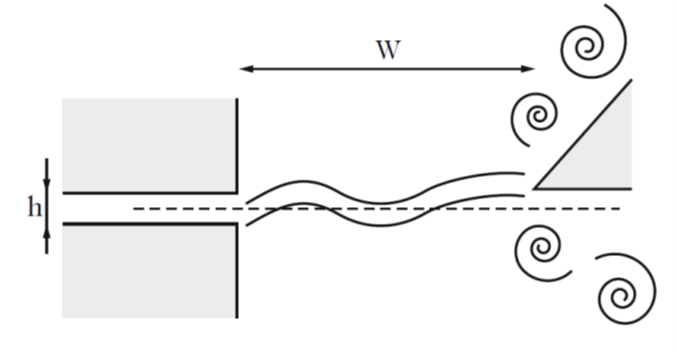
\includegraphics[width=0.4\textwidth]{images/7_20_1.png}
\end{figure}

When additional acoustic energy is introduced through the turbulent jet, it enters an environment already dominated by this resonant frequency. Due to jet receptivity, the jet aligns its dynamics with the pre-existing acoustic field in the chamber. The sharp edge, acting as a secondary source, produces oscillations that are directly influenced by the frequency already present in the chamber.

\begin{figure}[H]
    \centering
    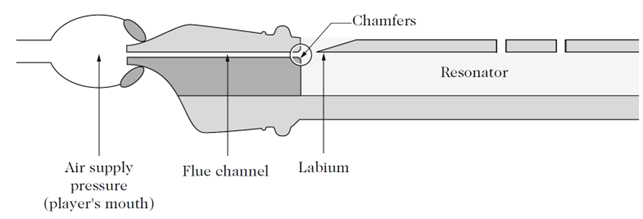
\includegraphics[width=0.6\textwidth]{images/7_20_2.png}
\end{figure}





This process creates a positive feedback loop: the primary airflow (jet) enters the pipe, which itself is a resonant chamber. If we were to introduce white noise into this chamber, it would act as a passive filter, allowing only its natural resonant frequency to remain, though weakly. However, in steady-state conditions, the chamber is already filled with an acoustic field oscillating at its specific resonant frequency, and this existing field actively influences the behavior of the jet. When the sharp edge creates a secondary source, it does not produce a broadband or random source but instead oscillates at the exact resonant frequency of the chamber. This happens because the jet, being receptive to the acoustic environment, aligns itself with the dominant frequency of the chamber. The cavity, far from being a passive filter, actively participates in the generation of sound, shaping the dynamics of the jet and the sharp edge. As a result, energy is efficiently channeled into this specific frequency, leading to a build-up of energy and amplification of the resonant tone. \begin{figure}[H]
    \centering
    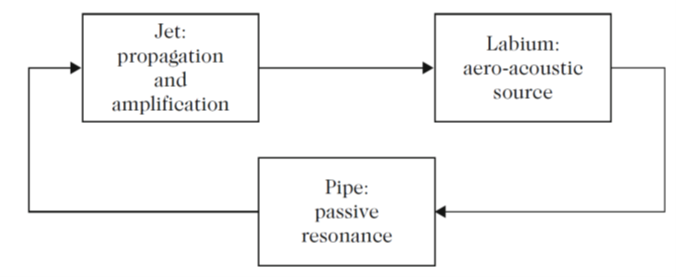
\includegraphics[width=0.5\textwidth]{images/7_20_3.png}
\end{figure}

\subsection{Turbulence}
To describe the behavior of fluid flow inside a system, particularly the transition between laminar and turbulent flow, we use the Reynolds number (\( Re \)). This dimensionless number represents the ratio between inertial forces and viscous forces in the fluid. It is given by the formula:

\[
Re = \frac{U_j h}{\nu},
\]

where:
\begin{itemize}
    \item    \( U_j \) is the mean velocity of the fluid,
\item \( h \) is the characteristic length of the system (e.g., the diameter of a pipe),
\item  \( \nu \) is the kinematic viscosity of the fluid.
\end{itemize}
The viscosity of air is approximately \( \nu = 1.5 \cdot 10^{-5} \, \text{m}^2/\text{s} \). For Reynolds numbers within the range \( 500 < Re < 10,000 \), the system is prone to transitioning from laminar to turbulent behavior. 

A higher Reynolds number indicates a greater likelihood of turbulence. This tendency increases with higher velocities (\( U_j \)), larger characteristic lengths (\( h \) (e.g., pipes with greater diameters), or lower fluid viscosity (\( \nu \)). 
\begin{figure}[H]
    \centering
    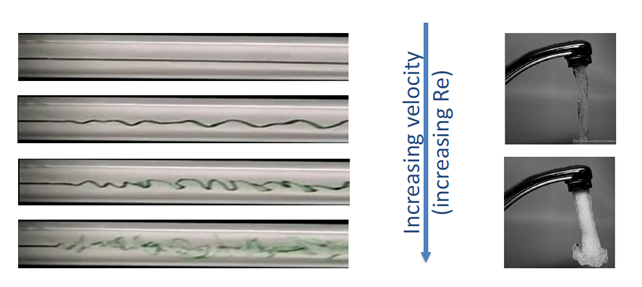
\includegraphics[width=0.8\textwidth]{images/7_22.png}
\end{figure}




As the flow of water increases, a transition occurs from a laminar flow to a turbulent flow. This behavior can be observed in everyday systems and has implications for various technologies.  If we consider a jet of ink injected into a pipe filled with water: at lower velocities, the ink moves straight through the pipe, maintaining a laminar flow; as the velocity of the water increases, the ink stream begins to exhibit turbulent behavior, spreading irregularly within the pipe.
In the example of water falling vertically, the diameter at the bottom of the stream is smaller than at the top. This occurs because, as the velocity of the water increases during its fall, the cross-sectional area of the stream decreases to conserve the flow rate (\( Q = \text{velocity} \times \text{cross-sectional area} \)).

    Modern microchip technologies rely on microfluidic channels for applications such as blood analysis. These channels are designed to transport fluids through extremely small cross-sections. In these systems, the cross-sectional dimensions are so small that the Reynolds number (\( Re \)) remains low, preventing the transition to turbulent flow. This laminar flow regime presents challenges for mixing two fluids effectively, as turbulence—a key driver for mixing—is absent.



\end{document} 

